\documentclass{article}

\usepackage{Stil}
\usepackage[utf8]{inputenc}
\usepackage{amsmath}
\usepackage{amsfonts}
\usepackage{amssymb}
\usepackage{graphicx}
\usepackage{float}
\usepackage{tikz}
\usepackage{listings}
\usepackage{color}
\usepackage{hyperref}
\usepackage{geometry}
\usepackage{tcolorbox}
\usepackage{qrcode}

% Python kod renklendirmesi için
\definecolor{codegreen}{rgb}{0,0.6,0}
\definecolor{codegray}{rgb}{0.5,0.5,0.5}
\definecolor{codepurple}{rgb}{0.58,0,0.82}
\definecolor{backcolour}{rgb}{0.95,0.95,0.92}

 \renewcommand{\abstractname}{Özet}

\lstdefinestyle{mystyle}{
    backgroundcolor=\color{backcolour},   
    commentstyle=\color{codegreen},
    keywordstyle=\color{magenta},
    numberstyle=\tiny\color{codegray},
    stringstyle=\color{codepurple},
    basicstyle=\ttfamily\footnotesize,
    breakatwhitespace=false,         
    breaklines=true,                 
    captionpos=b,                    
    keepspaces=true,                 
    numbers=left,                    
    numbersep=5pt,                  
    showspaces=false,                
    showstringspaces=false,
    showtabs=false,                  
    tabsize=2
}

\lstset{style=mystyle}

\title{Yapısal Optimizasyon Teknikleri}
\author{Bilal TAYFUR}

\begin{document}

\begin{titlepage}
\thispagestyle{empty}
\maketitle

\begin{abstract}
Bu ders, yapısal sistemlerin optimizasyonu konusunda kapsamlı bir giriş sunmaktadır. Öğrenciler, optimizasyon teorisinin temellerinden başlayarak, klasik ve modern optimizasyon yöntemlerinin genel farkını öğrenecek, yapısal sistemlerin tasarımında ve analizinde bu yöntemleri uygulama becerisi kazanacaklardır. 

Anlatılan konuların sağ tarafında verilen karekodlar üzerinden derse ait GitHub reposunda ilgili örneğin kodlarına erişilebilir. Bu repo her yıl güncellenmektedir. Dolayısıyla güncel ders notlarına ve yeni eklenen uygulamalara da repo üzerinden erişlebilir ve arzu edilirse katkı sağlanabilir.

\vspace{10pt}
\begin{center}
\qrcode[height=4cm]{https://github.com/btayfur/structural-optimization}
\end{center}




\vspace{10pt}
\noindent Bu ders kapsamında, aşağıdaki kaynak kitaplar konuları daha derinlemesine incelemek isteyen öğrencilere tavsiye edilmektedir:

\begin{itemize}
    \item Cottle, R. W., \& Thapa, M. N. (2017). \textbf{Linear and Nonlinear Optimization}. Springer.
    \item Rao, S. S. (2019). \textbf{Engineering Optimization: Theory and Practice, 5th Edition}. John Wiley \& Sons.
    \item Arora, J. S. (2016). \textbf{Introduction to Optimum Design, 4th Edition}. Academic Press.
    \item Yang, X. S. (2021). \textbf{Nature-Inspired Optimization Algorithms, 2nd Edition}. Elsevier.
    \item Bendsøe, M. P., \& Sigmund, O. (2003). \textbf{Topology Optimization: Theory, Methods, and Applications}. Springer.
\end{itemize}

\end{abstract}

\setcounter{tocdepth}{3}
\tableofcontents
\end{titlepage}

\newgeometry{top=20mm,bottom=25mm,right=80mm,left=20mm}

% Haftalık içeriklerin dahil edilmesi
\section{Optimizasyon Teorisine Giriş}
Optimizasyon teorisi, bir sistemin performansını belirli kısıtlar altında en iyi duruma getirmeyi amaçlayan matematiksel ve metodolojik yaklaşımların bütünüdür. Bu ders, yapısal sistemlerin optimizasyonuna odaklanarak, temel kavramları ve uygulama yöntemlerini ele alacaktır.

\subsection{Optimizasyonun Tanımı ve Mühendislikteki Önemi}
Optimizasyon, bir sistemin performansını belirli kısıtlar altında en iyi duruma getirme sürecidir. \sidenote{Günlük hayatta sıkça karşılaştığımız "en iyi" kararı verme süreçleri aslında birer optimizasyon problemidir. Örneğin, işe giderken en kısa yolu seçmek, market alışverişinde en uygun fiyatlı ürünleri tercih etmek gibi.} Bu süreç, mühendislik tasarımlarında maliyeti düşürürken performansı artırmayı hedefler.


\subsection{Yapısal Optimizasyonun Temel Bileşenleri}
Yapısal optimizasyon, üç temel bileşen üzerine kurulur: amaç fonksiyonu, tasarım değişkenleri ve kısıtlar. Bu bileşenler, optimizasyon probleminin matematiksel formülasyonunu oluşturur.

\begin{itemize}
    \item \textbf{Amaç Fonksiyonu:} Minimize veya maksimize edilmek istenen hedef (örn. ağırlık, maliyet, rijitlik)
    \item \textbf{Tasarım Değişkenleri:} Optimize edilecek parametreler (örn. kesit boyutları, malzeme özellikleri)
    \item \textbf{Kısıtlar:} Tasarımın sağlaması gereken koşullar (örn. gerilme limitleri, deplasman sınırları)
\end{itemize}

\begin{marginfigure}
\centering
\begin{tikzpicture}
\draw[->] (0,0) -- (4,0) node[right] {$x_i$};
\draw[->] (0,0) -- (0,3) node[above] {$F(x)$};
\draw[scale=1,domain=0.5:3.5,smooth,variable=\x,blue] plot ({\x},{2.5*exp(-0.5*(\x-2)^2)});
\draw[red,dashed] (2,0) -- (2,2.5);
\filldraw[red] (2,2.5) circle (2pt) node[above] {Optimum};
\end{tikzpicture}
\caption{Tek değişkenli bir optimizasyon probleminde optimum noktanın gösterimi}
\label{fig:single_var_opt}
\end{marginfigure}

\subsection{Optimizasyonun Tarihçesi ve Gelişimi}
Optimizasyon teorisinin temelleri, matematiksel analiz yöntemlerinin gelişimiyle paralel olarak ilerlemiştir. Modern optimizasyon yöntemleri, bilgisayar teknolojisinin gelişimiyle birlikte yeni boyutlar kazanmıştır. \sidenote{İlk yapısal optimizasyon çalışmaları, Michell'in 1904'te yayınladığı kafes sistemlerin minimum ağırlık tasarımı ile başlamıştır. Bu çalışma, modern topoloji optimizasyonunun temelini oluşturur.}

\subsubsection{Önemli Tarihsel Gelişmeler}
\begin{itemize}
    \item 1940'lar: Doğrusal programlama ve Simplex metodunun geliştirilmesi
    \item 1950'ler: Dinamik programlama ve konveks optimizasyon teorisi
    \item 1960'lar: Sonlu elemanlar yönteminin optimizasyona uygulanması
    \item 1970'ler: Sayısal optimizasyon algoritmalarının geliştirilmesi
    \item 1980'ler: Metasezgisel algoritmaların ortaya çıkışı
    \item 1990'lar: Topoloji optimizasyonunun yaygınlaşması
    \item 2000'ler: Çok amaçlı optimizasyon ve yapay zeka tekniklerinin entegrasyonu
\end{itemize}

\subsection{Optimizasyon Problemlerinin Genel Yapısı}
Her optimizasyon problemi, bir amaç fonksiyonunun minimizasyonu veya maksimizasyonu şeklinde ifade edilir. Problem formülasyonu, tasarım değişkenlerini ve kısıtları içerir. \sidenote{Optimizasyon probleminin matematiksel formülasyonu, problemi sistematik bir şekilde çözebilmemiz için gerekli olan yapıyı sağlar. Bu formülasyon, farklı mühendislik problemlerini ortak bir çerçevede ele almamıza olanak tanır.}

\begin{equation}
\begin{aligned}
& \text{minimize} & & f(\mathbf{x}) \\
& \text{subject to} & & g_i(\mathbf{x}) \leq 0, & & i = 1,\ldots,m \\
& & & h_j(\mathbf{x}) = 0, & & j = 1,\ldots,p \\
& & & x_k^L \leq x_k \leq x_k^U, & & k = 1,\ldots,n
\end{aligned}
\end{equation}

\begin{tcolorbox}[title=Yapısal Optimizasyon Örneği]
Bir çelik kirişin optimum tasarımı için:
\begin{itemize}
    \item \textbf{Amaç:} Minimum ağırlık
    \item \textbf{Değişkenler:} Kesit yüksekliği ve genişliği
    \item \textbf{Kısıtlar:} 
        \begin{itemize}
            \item Maksimum gerilme $\leq$ Akma gerilmesi
            \item Maksimum sehim $\leq$ İzin verilen sehim
            \item Minimum kesit boyutları
        \end{itemize}
\end{itemize}
\end{tcolorbox}

\subsection{Optimizasyonun Mühendislikteki Temel Uygulama Alanları}
Optimizasyon, mühendisliğin çeşitli alanlarında yaygın olarak kullanılır. İnşaat, makine, havacılık ve uzay mühendisliği başlıca uygulama alanlarıdır.

\begin{itemize}
    \item \textbf{İnşaat Mühendisliği:}
        \begin{itemize}
            \item Çelik yapıların kesit optimizasyonu
            \item Betonarme elemanların donatı optimizasyonu
            \item Köprü tasarımında form optimizasyonu
        \end{itemize}
    \item \textbf{Makine Mühendisliği:}
        \begin{itemize}
            \item Mekanik parçaların şekil optimizasyonu
            \item Termal sistemlerin performans optimizasyonu
            \item Titreşim kontrolü ve sönümleme
        \end{itemize}
    \item \textbf{Havacılık ve Uzay Mühendisliği:}
        \begin{itemize}
            \item Kanat ve gövde tasarımı
            \item Kompozit malzeme optimizasyonu
            \item Yapısal ağırlık minimizasyonu
        \end{itemize}
\end{itemize}


\subsection{Deterministik ve Stokastik Optimizasyon Yaklaşımları}
Optimizasyon yöntemleri, problem çözme yaklaşımlarına göre deterministik \sidenote{Deterministik bir yöntemin, her çalıştırmada aynı sonucu vermesi gerektiği anlamına gelir. Yani stabil ve öngörülebilirdirler.} ve stokastik \sidenote{Stokastik ise bir yöntemin, her çalıştırmada farklı sonuçlar üretebilmesi gerektiği anlamına gelir. Yani rastgele ve öngörülemez (daha doğrusu öngörüsü kısıtlı) bir yöntemdir.} olmak üzere iki ana kategoriye ayrılır. 

\subsubsection{Deterministik Yaklaşımlar}
\begin{itemize}
    \item Her çalıştırmada aynı sonucu verir
    \item Gradyan tabanlı yöntemler bu kategoridedir
    \item Lokal optimuma takılma riski vardır
    \item Başlangıç noktasına bağımlıdır
\end{itemize}

\subsubsection{Stokastik Yaklaşımlar}
\begin{itemize}
    \item Rastgelelik içerir
    \item Her çalıştırmada farklı sonuçlar üretebilir
    \item Global optimumu bulma olasılığı daha yüksektir
    \item Genetik algoritmalar, tavlama benzetimi gibi yöntemler bu kategoridedir
\end{itemize}

Bu yaklaşımlar, farklı problem tiplerine uygun çözüm stratejileri sunar. \sidenote{Deterministik ve stokastik yaklaşımların seçimi, problemin yapısına ve çözüm gereksinimlerine bağlıdır. Örneğin, çok modlu bir problemde stokastik yöntemler daha avantajlı olabilir.}

\subsection{Doğrusal ve Doğrusal Olmayan Optimizasyon}
Optimizasyon problemleri, amaç fonksiyonu ve kısıtların yapısına göre doğrusal ve doğrusal olmayan problemler olarak sınıflandırılır. Bu sınıflandırma, kullanılacak çözüm yöntemlerini belirler.

\subsubsection{Doğrusal Optimizasyon}
\begin{itemize}
    \item Amaç fonksiyonu ve kısıtlar doğrusaldır
    \item Çözüm uzayı konvekstir
    \item Simplex metodu gibi etkin çözüm yöntemleri vardır
    \item Global optimum garanti edilir
\end{itemize}

\begin{tcolorbox}[title=Doğrusal Optimizasyon Örneği]
Bir üretim planlaması problemi:
\begin{equation*}
\begin{aligned}
\text{maximize} \quad & 3x_1 + 2x_2 \\
\text{subject to} \quad & 2x_1 + x_2 \leq 100 \\
& x_1 + x_2 \leq 80 \\
& x_1, x_2 \geq 0
\end{aligned}
\end{equation*}
\end{tcolorbox}

\subsubsection{Doğrusal Olmayan Optimizasyon}
\begin{itemize}
    \item Amaç fonksiyonu ve/veya kısıtlar doğrusal değildir
    \item Çözüm uzayı karmaşıktır
    \item Lokal optimumlar içerebilir
    \item Yapısal problemlerin çoğu bu kategoridedir \sidenote{Yapısal mühendislikte karşılaşılan problemlerin büyük çoğunluğu doğrusal olmayan karakterdedir. Örneğin, geometrik nonlineerite, malzeme nonlineeritesi gibi etkiler problemi doğrusal olmayan hale getirir.}
\end{itemize}

\begin{tcolorbox}[title=Doğrusal Olmayan Optimizasyon Örneği]
    Bir yapısal tasarım optimizasyonu problemi:
    \begin{equation*}
    \begin{aligned}
    \text{minimize} \quad & f(x) = x_1^2 + 2x_2^2 - 0.3x_1x_2 \\
    \text{subject to} \quad & g_1(x) = x_1^2 + x_2^2 - 25 \leq 0 \\
    & g_2(x) = x_1 - 2x_2 + 5 \leq 0 \\
    & -10 \leq x_1, x_2 \leq 10
    \end{aligned}
    \end{equation*}
    \end{tcolorbox}



\subsection{Çözüm Yöntemlerinin Genel Sınıflandırılması}
Optimizasyon yöntemleri, problem tipine ve çözüm stratejisine göre analitik, sayısal ve metasezgisel yöntemler olarak sınıflandırılır. Her yöntem grubu, belirli problem tipleri için avantajlar sunar.

\begin{itemize}
    \item \textbf{Analitik Yöntemler}
        \begin{itemize}
            \item Diferansiyel hesap
            \item Varyasyonel yöntemler
            \item Lagrange çarpanları
        \end{itemize}
    \item \textbf{Sayısal Yöntemler}
        \begin{itemize}
            \item Gradyan tabanlı yöntemler
            \item Doğrusal programlama
            \item Nonlineer programlama
        \end{itemize}
    \item \textbf{Metasezgisel Yöntemler}
        \begin{itemize}
            \item Genetik algoritmalar
            \item Parçacık sürü optimizasyonu
            \item Tavlama benzetimi
        \end{itemize}
\end{itemize}

\subsection{Optimizasyon Problemlerinde Global ve Lokal Optimumlar}

Çok modlu optimizasyon problemlerinde, birden fazla lokal optimum noktası bulunabilir. Bu durum, özellikle doğrusal olmayan problemlerde sıklıkla karşımıza çıkar.

\begin{figure}[H]
    \centering
    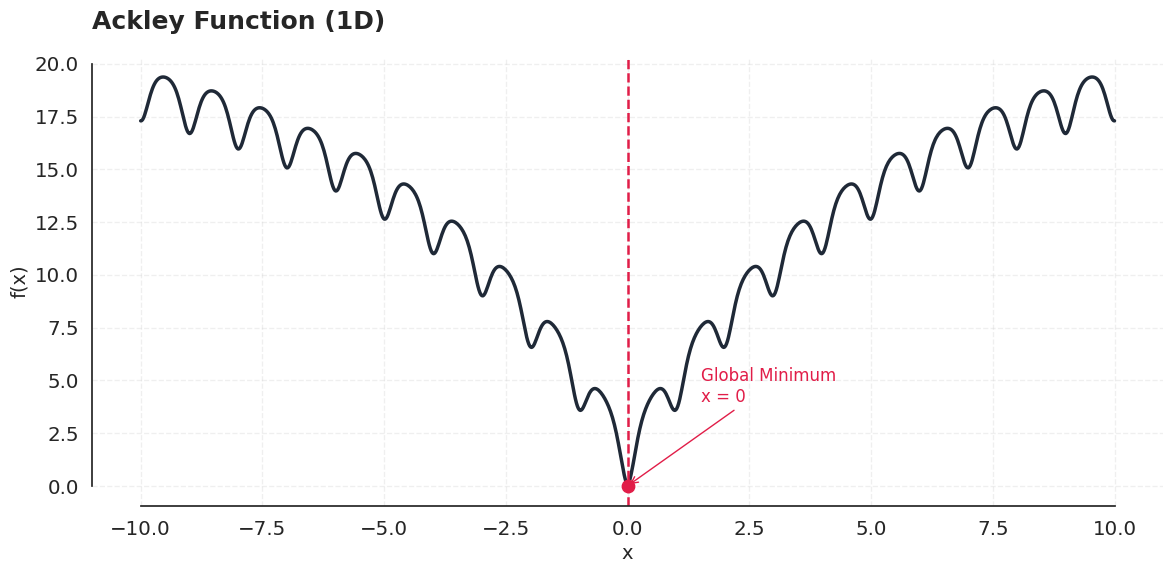
\includegraphics[width=\textwidth]{weeks_new/imgs/multi_mod.png}
    \caption{Tek boyutlu ve çok modlu optimizasyon problemi}
    \label{fig:multi_mod}
\end{figure}

Yukarıdaki şekilde görüldüğü gibi, çok modlu bir fonksiyonda birden fazla tepe (maksimum) ve çukur (minimum) noktası bulunabilir. Optimizasyon algoritmaları, başlangıç noktasına bağlı olarak lokal bir optimuma takılabilir ve global optimumu bulamayabilir. Bu nedenle, özellikle karmaşık mühendislik problemlerinde global optimumu bulmak için metasezgisel yöntemler tercih edilebilir.  
\section{Basic Optimization Concepts}
The fundamental concepts necessary for the mathematical formulation and solution of optimization problems will be examined in detail in this section. These concepts form the foundation for understanding more complex optimization problems.

\subsection{Objective Function and Constraint Functions}

In the mathematical modeling of optimization problems, there are two fundamental components: the objective function and constraint functions.

\subsubsection{Objective Function}
The objective function mathematically expresses the performance criterion to be optimized. This function can be:
\begin{itemize}
    \item Minimized (e.g., cost, weight, energy consumption)
    \item Maximized (e.g., efficiency, strength, stiffness)
\end{itemize}

\begin{figure}[H]
    \centering
    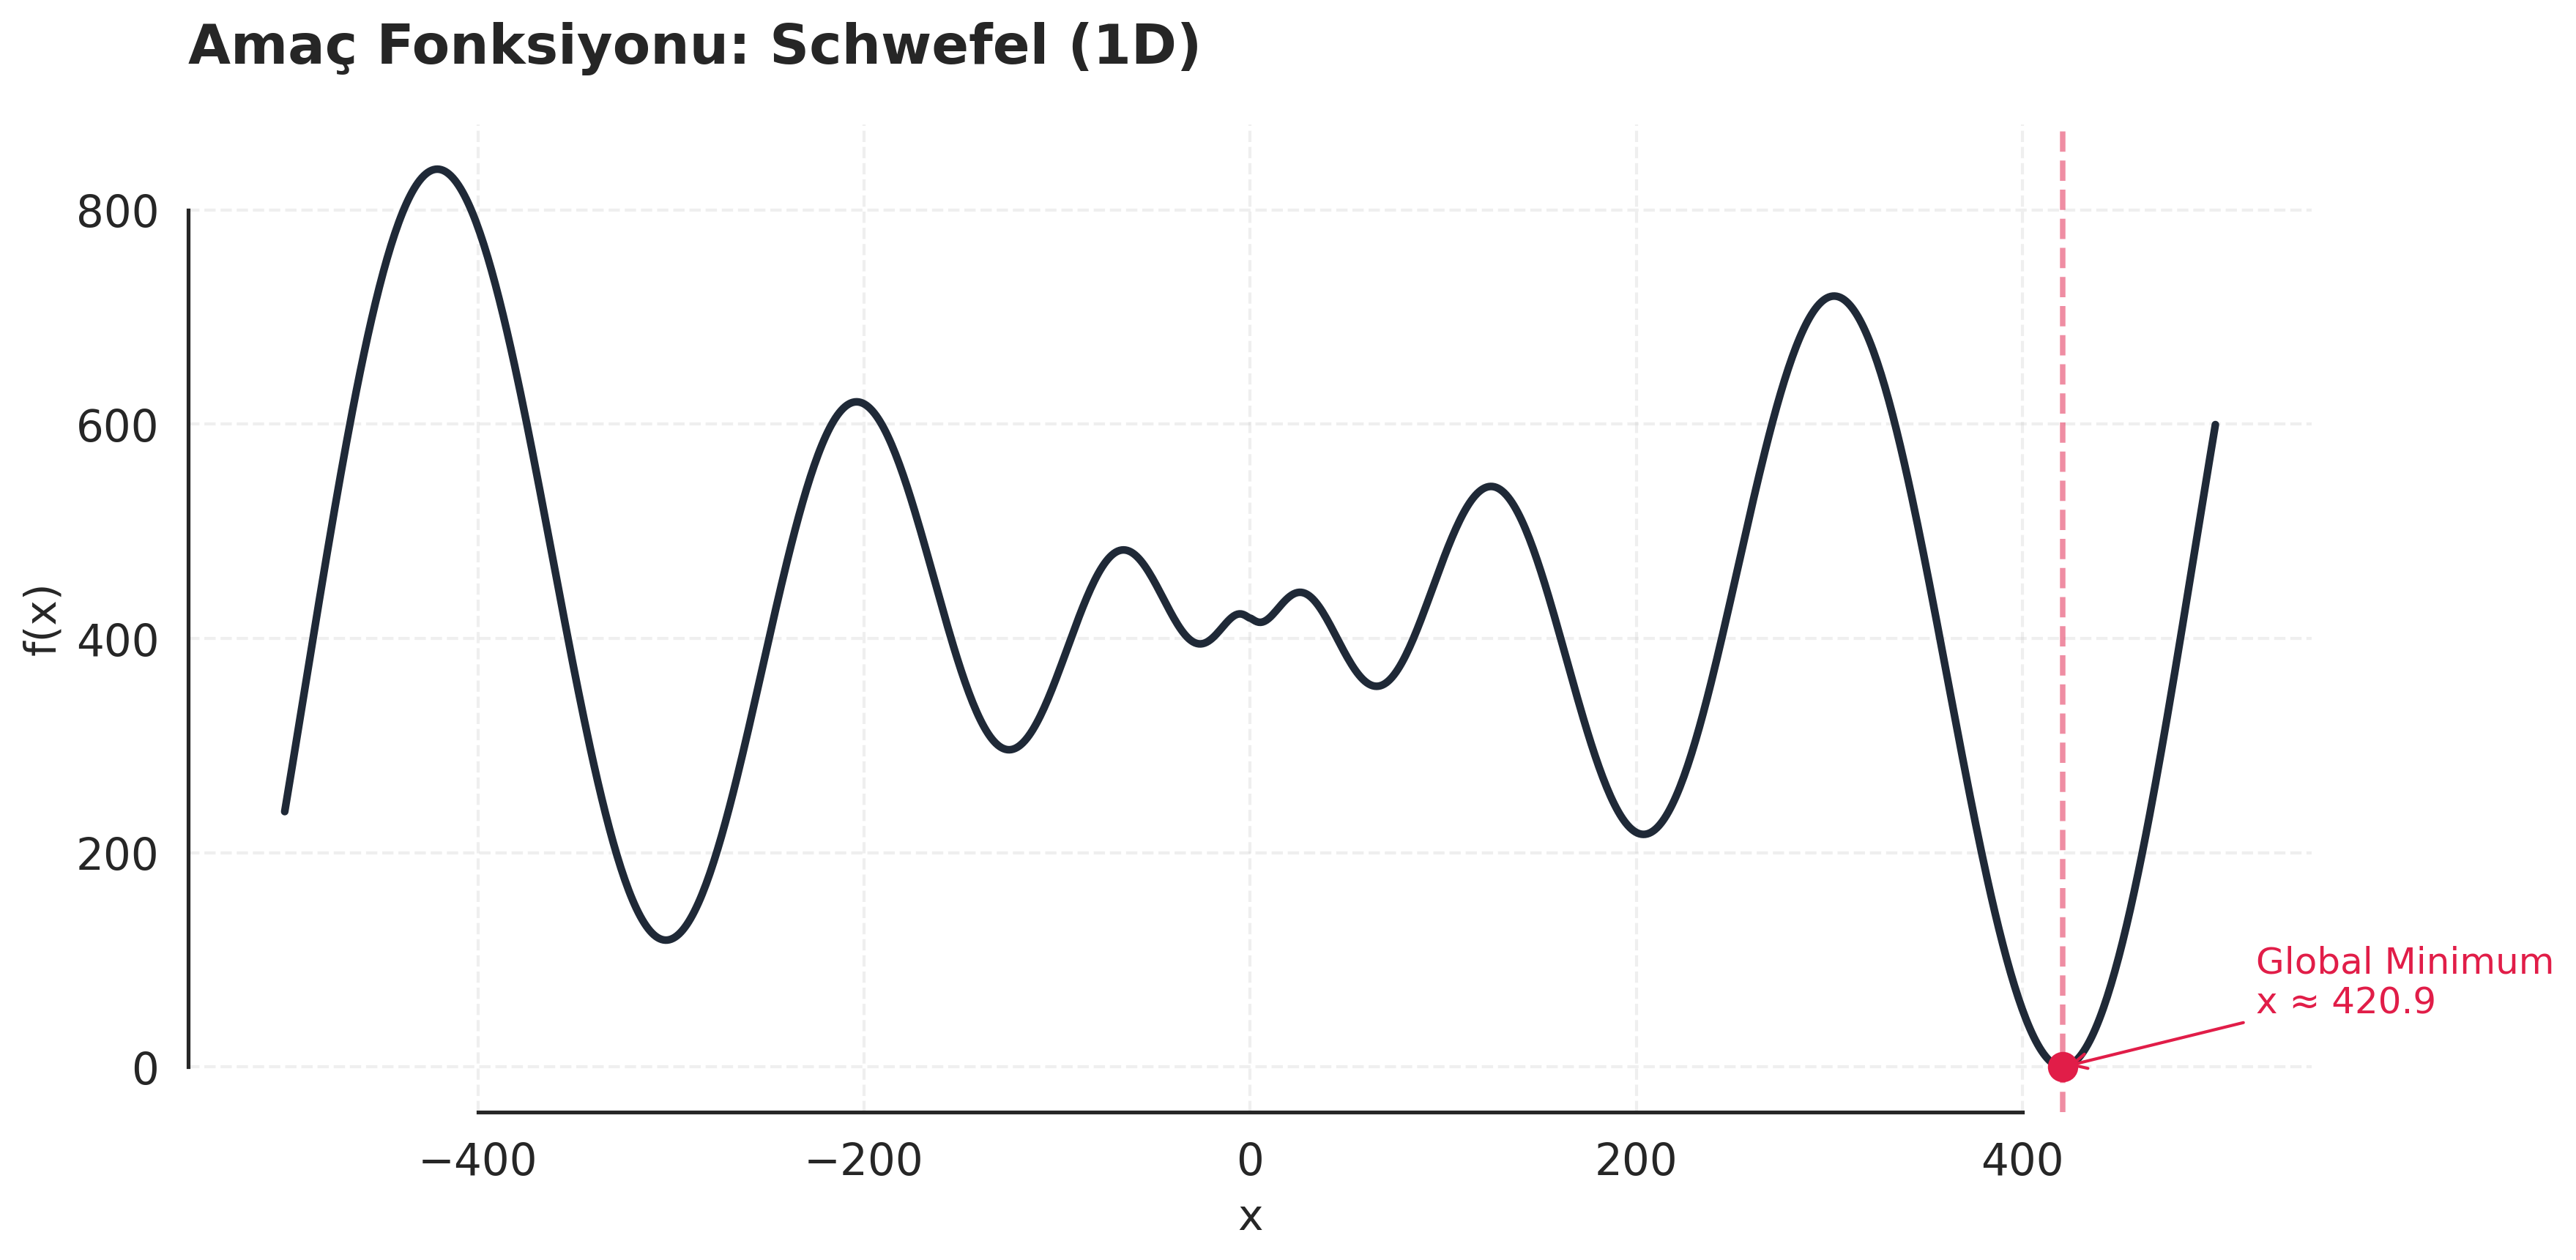
\includegraphics[width=1\textwidth]{weeks_new/imgs/objective_function.png}
    \caption{Objective Function}
    \label{fig:multi_mod}
\end{figure}

\sidenote{Any maximization problem can be converted to a minimization problem by taking the negative of the objective function: \[ \max f(x) = -\min(-f(x)) \]}

\subsubsection{Constraint Functions}
Constraint functions mathematically express the conditions that the design must satisfy:
\begin{itemize}
    \item Equality constraints: $h_j(x) = 0$
    \item Inequality constraints: $g_i(x) \leq 0$
    \item Boundary constraints: $x_L \leq x \leq x_U$ \sidenote{With few exceptions, structural optimization problems are generally expressed with inequality constraints. Depending on the problem, boundary constraints may also be used. However, when a statically indeterminate structure is subject to optimization, this constraint can also lead to missing the global optimum.
    
    In fact, one of the aspects that makes structural optimization problems worth examining from an optimization perspective is that this statical indeterminacy significantly increases the unpredictability of many structural optimization problems.}
\end{itemize}

\textbf{Equality constraints: $h_j(x) = 0$}
Equality constraints express situations where design variables must take exactly specific values. These types of constraints mathematically define conditions where certain parameters must be precisely satisfied within the optimization problem. For example, a structure's total weight being equal to a specific value or mass balance in a chemical reaction can be expressed with equality constraints. Equality constraints generally keep the optimization space in a narrower area, significantly reducing the number of possible solutions.

\begin{figure}[H]
    \centering
    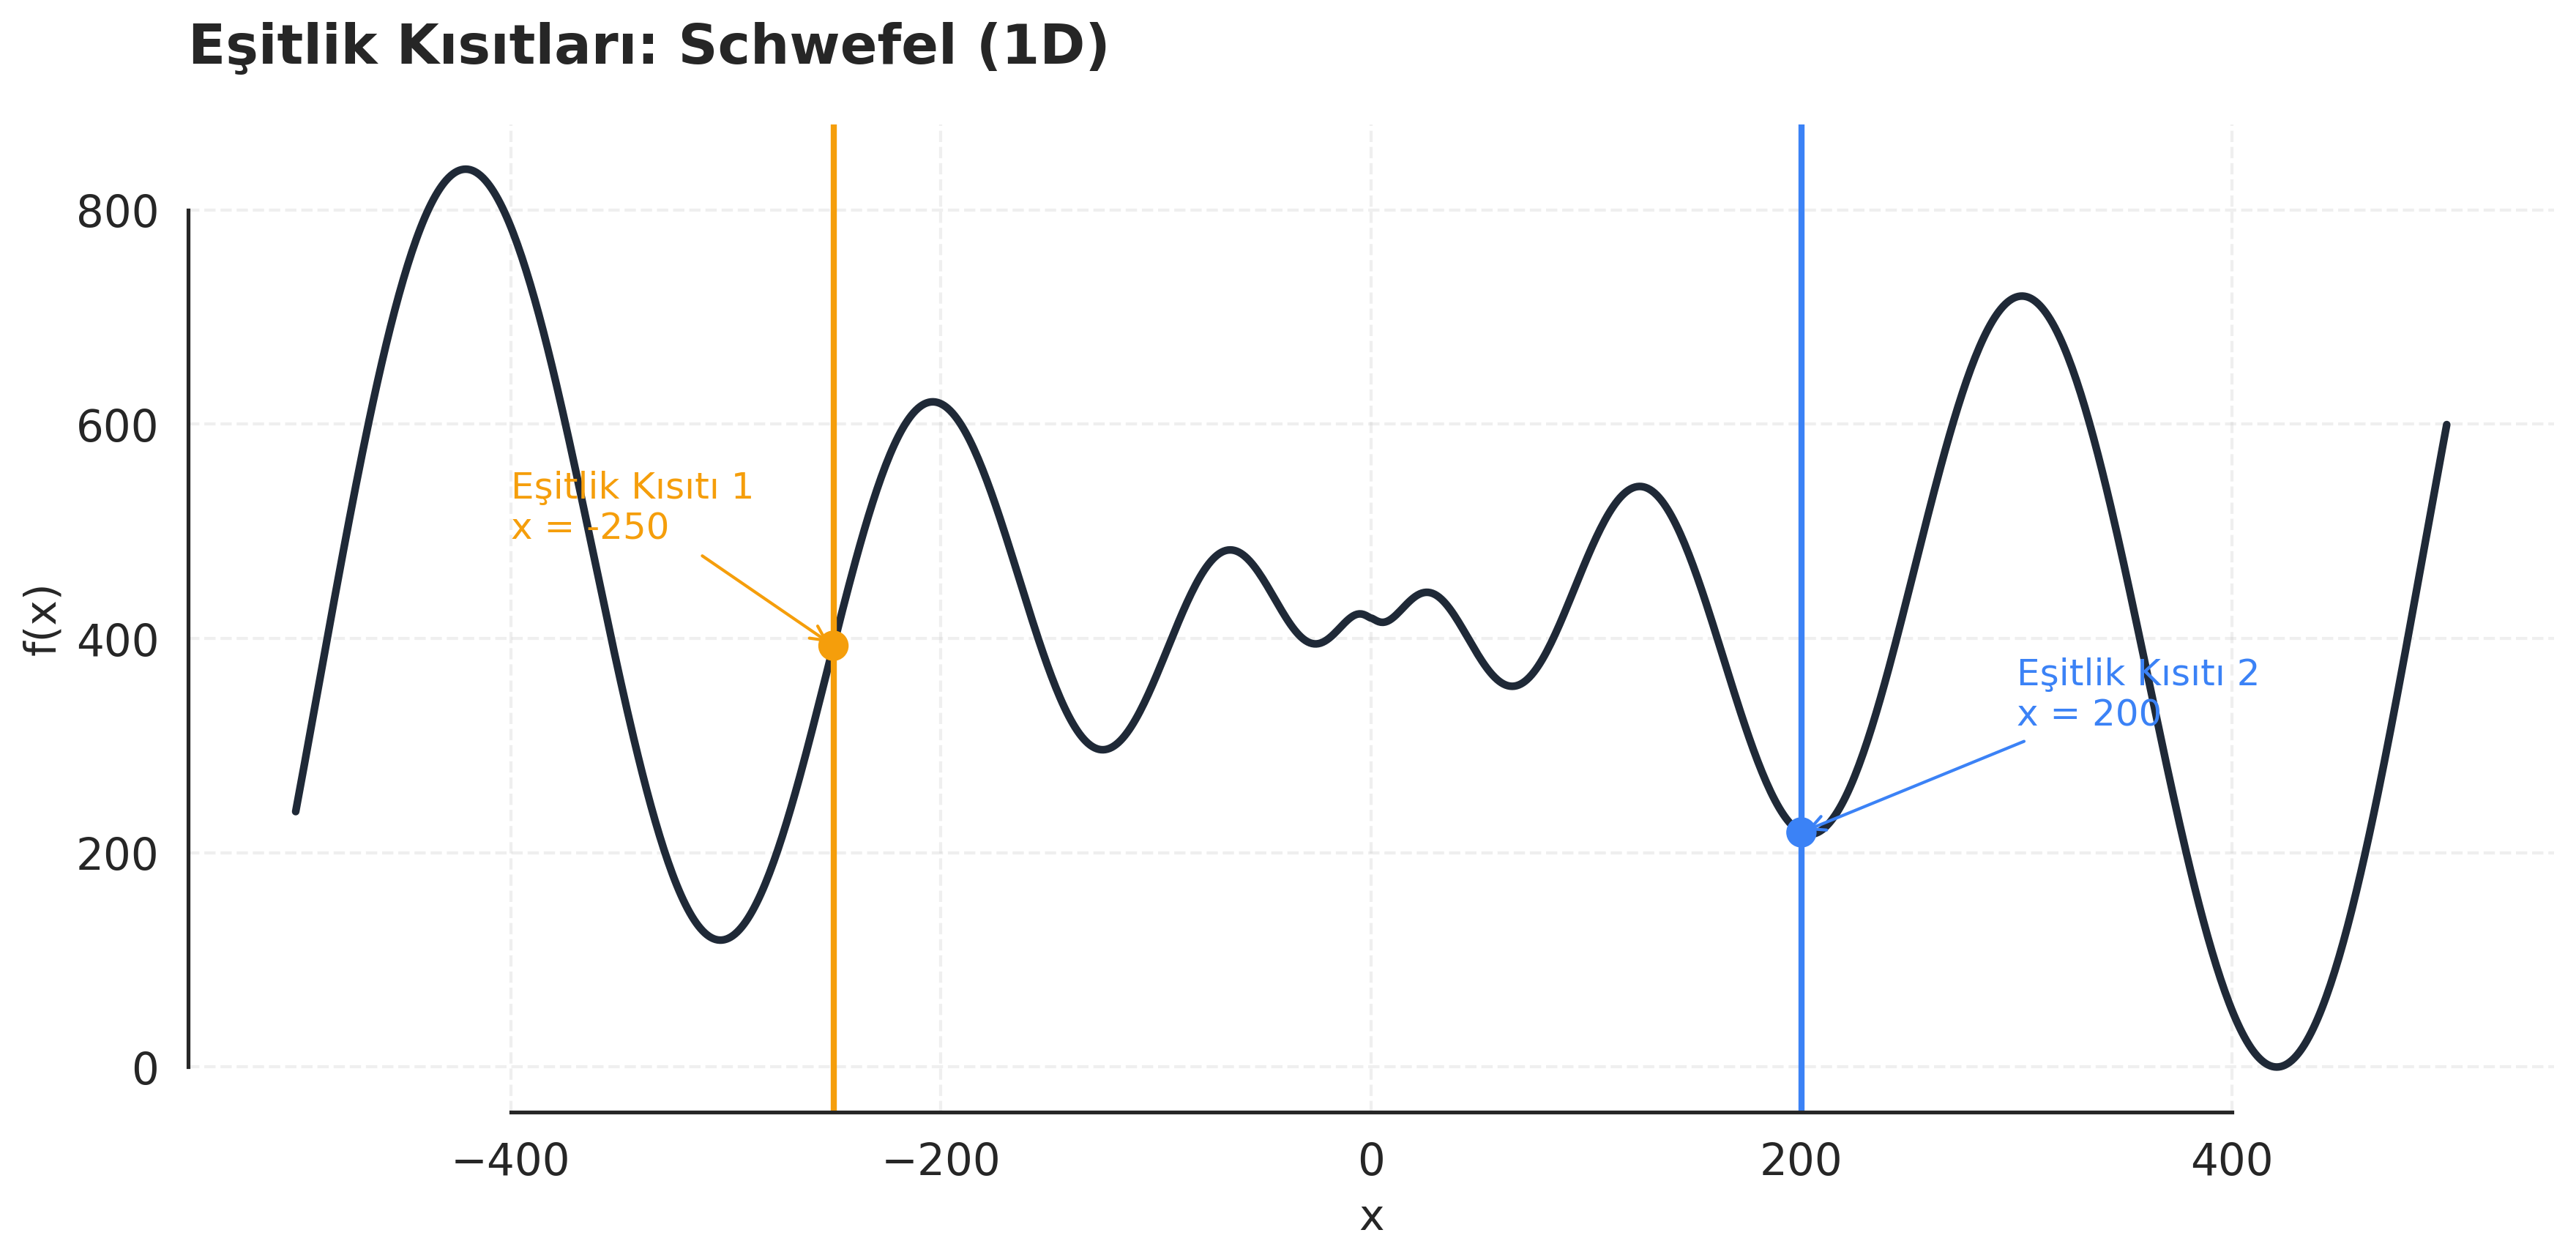
\includegraphics[width=1\textwidth]{weeks_new/imgs/equality_constraints.png}
    \caption{Equality Constraints}
    \label{fig:}
\end{figure}

\textbf{Inequality constraints: $g_i(x) \leq 0$}
Inequality constraints express situations where design variables must not exceed certain limits. These types of constraints are used to define limitations such as the maximum stress a structure can withstand, a system's maximum energy consumption, or a material's minimum safety factor. Inequality constraints are critical for ensuring that the design is physically realizable and safe. Additionally, inequality constraints define the feasible solution area, ensuring that the optimization algorithm searches only within the valid design space.

\begin{figure}[H]
    \centering
    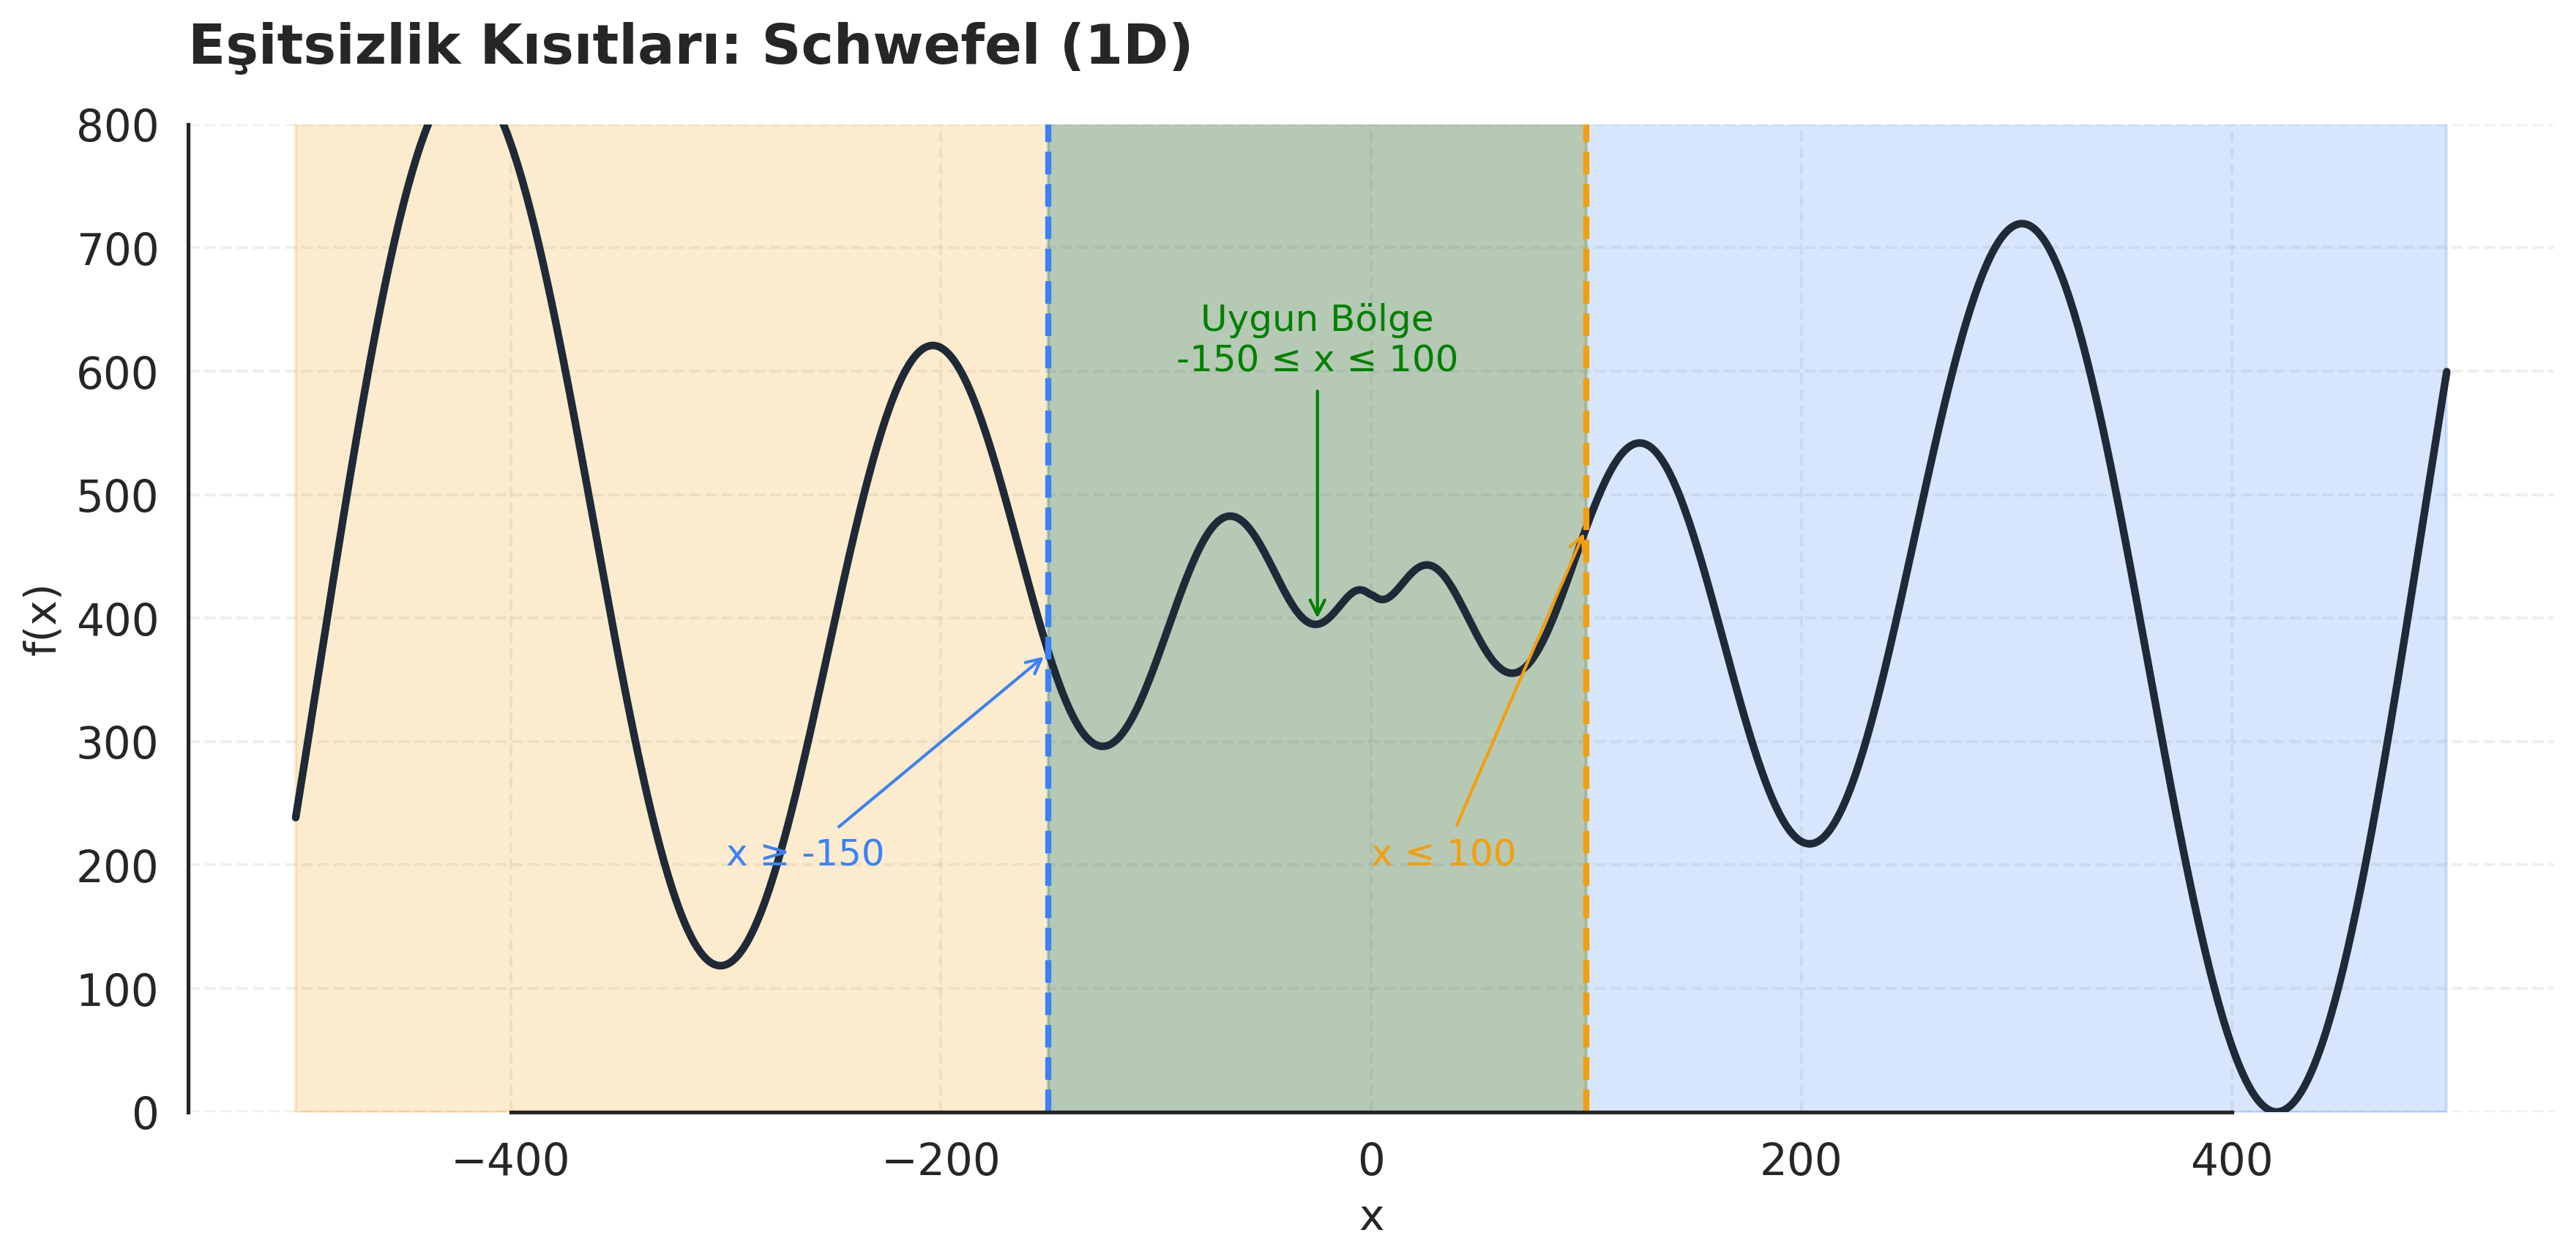
\includegraphics[width=1\textwidth]{weeks_new/imgs/inequality_constraints.png}
    \caption{Inequality Constraints}
    \label{fig:}
\end{figure}

\textbf{Boundary constraints: $x_L \leq x \leq x_U$}
Boundary constraints determine the minimum and maximum values that each design variable can take. These constraints reflect the physical limits of design variables, manufacturability conditions, or ranges determined by standards. For example, situations where a beam's thickness cannot be less than a certain value due to manufacturing constraints or cannot exceed a certain maximum value due to installation requirements are expressed with boundary constraints. Boundary constraints narrow the optimization algorithm's search space, increasing computational efficiency and ensuring the elimination of physically meaningless solutions.

\begin{figure}[H]
    \centering
    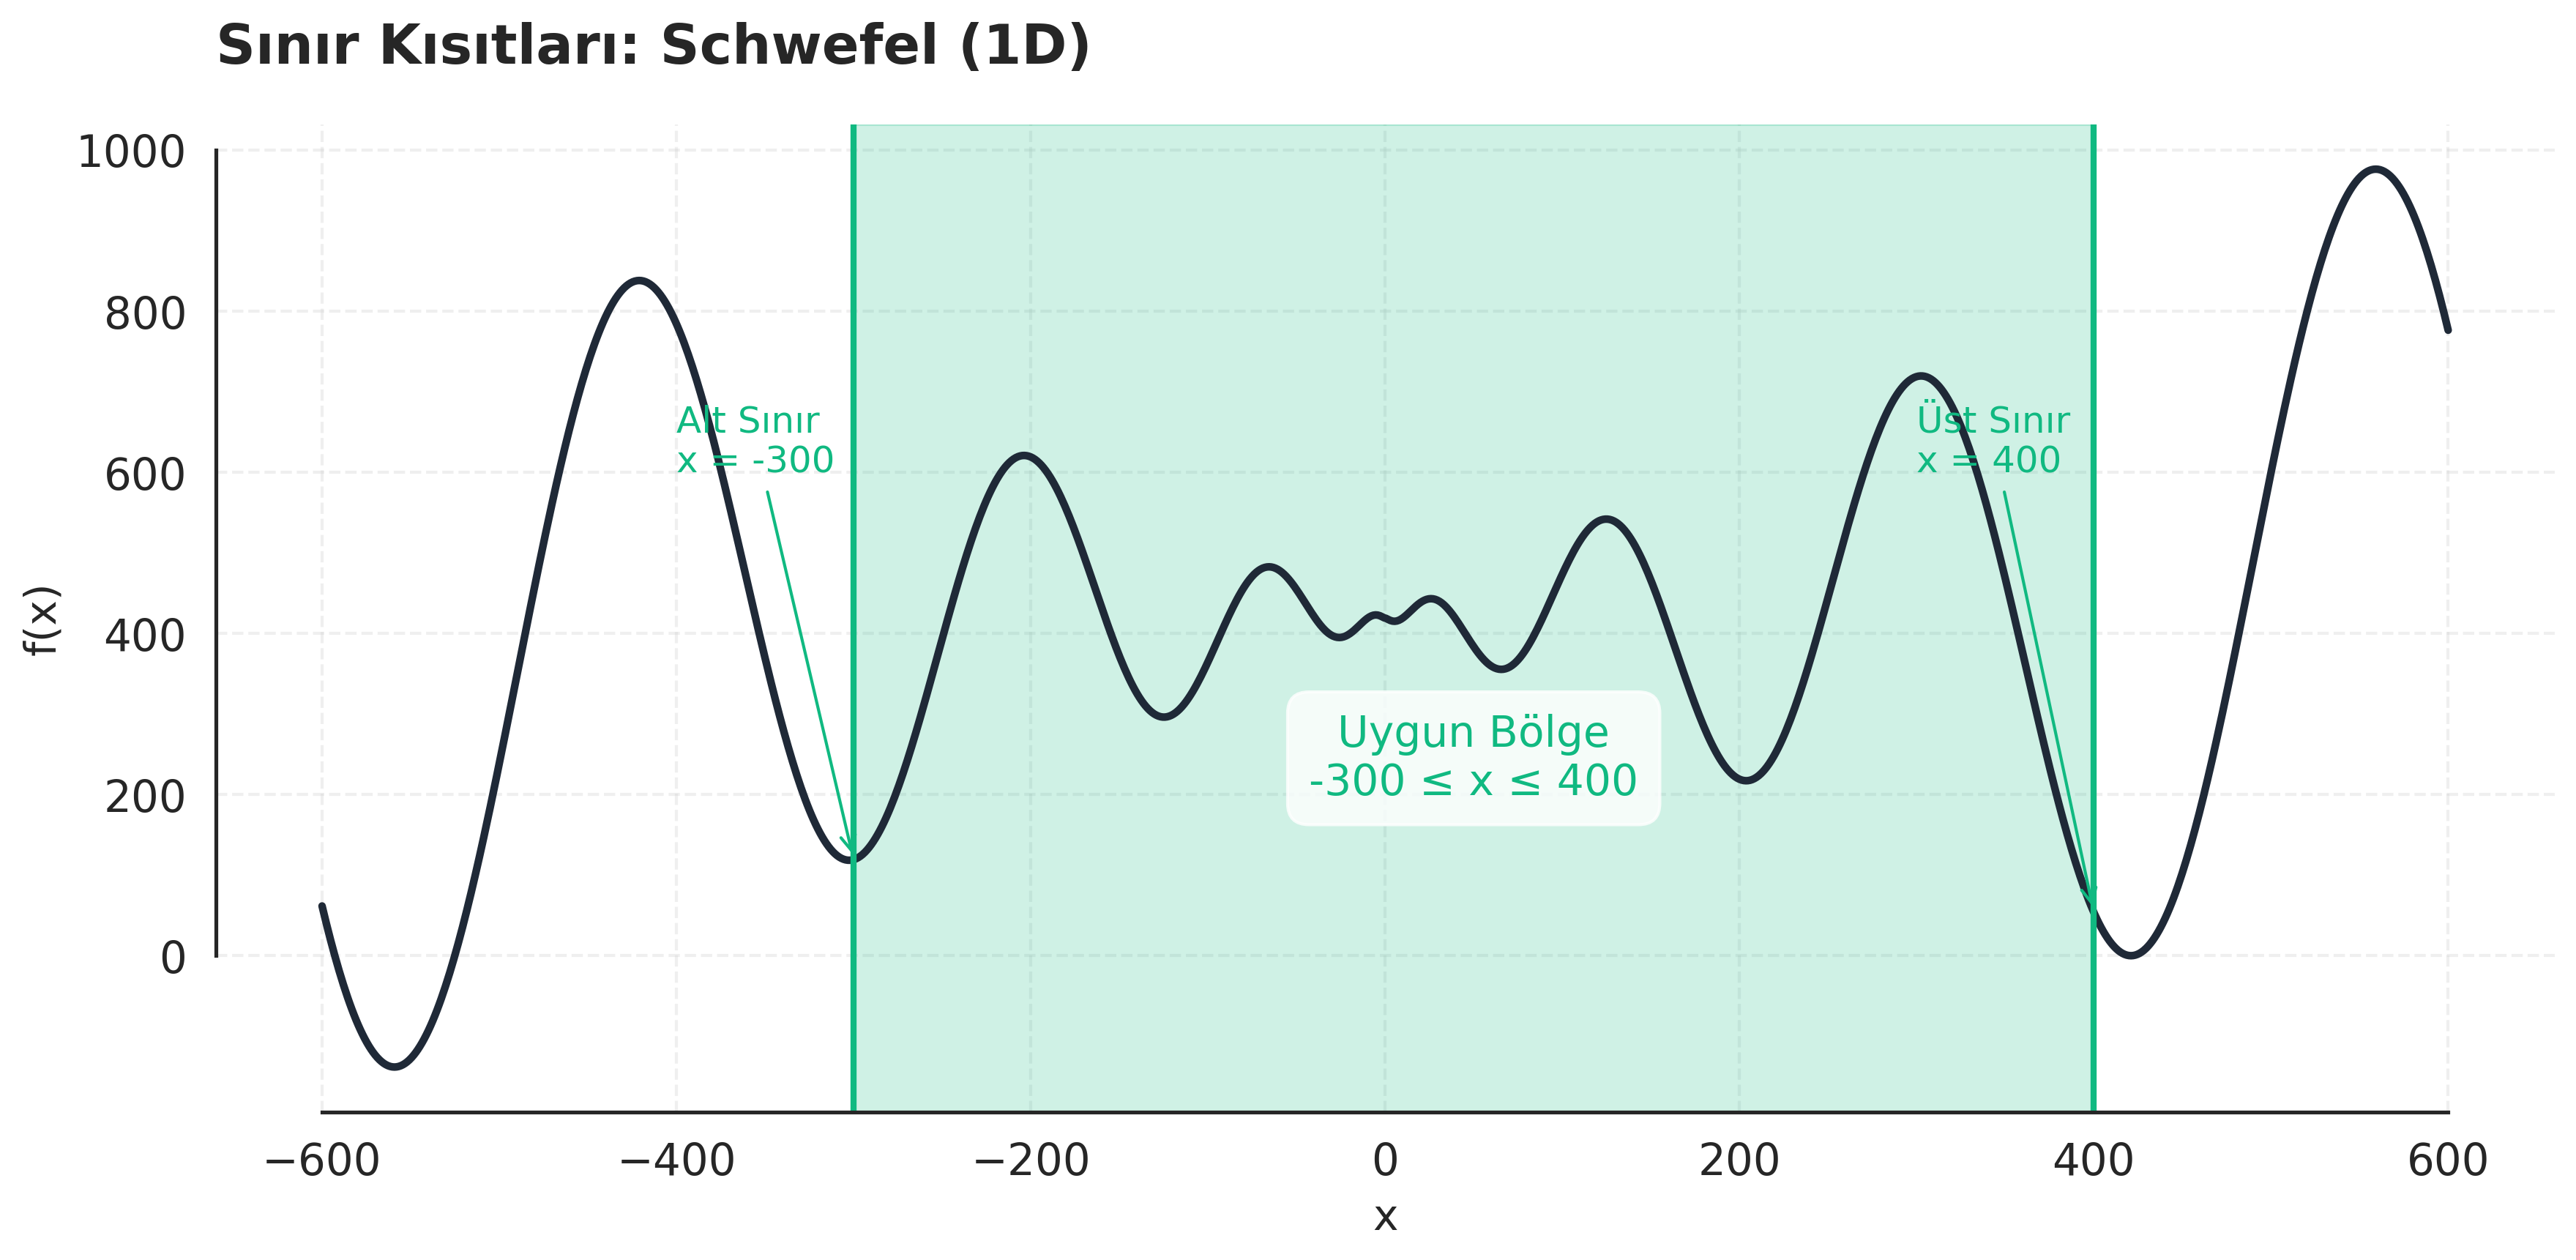
\includegraphics[width=1\textwidth]{weeks_new/imgs/boundary_constraints.png}
    \caption{Boundary Constraints}
    \label{fig:}
\end{figure}

\begin{marginfigure}
\centering
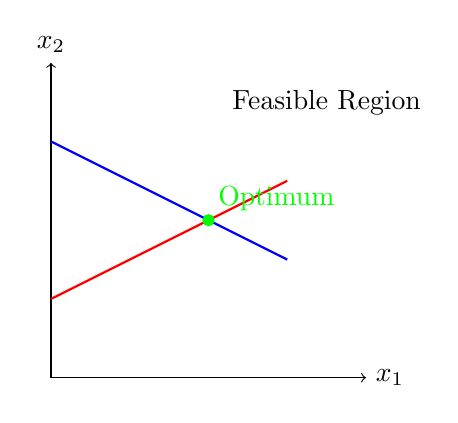
\begin{tikzpicture}
\draw[->] (0,0) -- (4,0) node[right] {$x_1$};
\draw[->] (0,0) -- (0,4) node[above] {$x_2$};
\draw[blue,thick] plot[smooth] coordinates {(0,3) (1,2.5) (2,2) (3,1.5)};
\draw[red,thick] plot[smooth] coordinates {(0,1) (1,1.5) (2,2) (3,2.5)};
\filldraw[green] (2,2) circle (2pt) node[above right] {Optimum};
\node at (3.5,3.5) {Feasible Region};
\end{tikzpicture}
\caption{Feasible solution region formed by the intersection of two constraints}
\label{fig:feasible_region}
\end{marginfigure}

\subsection{Decision Variables and Solution Space}

\subsubsection{Decision Variables}
Decision variables are parameters whose values need to be determined during the optimization process:
\begin{itemize}
    \item Continuous variables (e.g., dimensions, thicknesses)
    \item Discrete variables (e.g., number of elements)
    \item Binary variables (0-1 decisions)
\end{itemize}

\begin{tcolorbox}[title=Decision Variables in Structural Design]
In a steel frame optimization:
\begin{itemize}
    \item \textbf{Continuous:} Section dimensions
    \item \textbf{Discrete:} Number of stories
    \item \textbf{Binary:} Existence/non-existence of elements
\end{itemize}
\end{tcolorbox}

\subsubsection{Solution Space}
The solution space is the space formed by all possible combinations of decision variables\sidenote{The dimension of the solution space is determined by the number of decision variables. In high-dimensional problems, the "curse of dimensionality" problem arises.}:
\begin{itemize}
    \item \textbf{Feasible Solution Region:} Set of points satisfying all constraints
    \item \textbf{Infeasible Region:} Points violating at least one constraint
\end{itemize}

\subsection{Global and Local Minimum/Maximum Concepts}

\subsubsection{Local Optimum}
A point is a local optimum if it has the best value within a certain neighborhood:
\begin{equation}
x^* \text{ local minimum } \Leftrightarrow f(x^*) \leq f(x), \forall x \in N(x^*)
\end{equation}

\subsubsection{Global Optimum}
The point with the best value in the entire solution space is the global optimum:
\begin{equation}
x^* \text{ global minimum } \Leftrightarrow f(x^*) \leq f(x), \forall x \in S
\end{equation}

\begin{figure}
\centering
\begin{tikzpicture}
\draw[->] (0,0) -- (7,0) node[right] {$x$};
\draw[->] (0,-1) -- (0,4) node[above] {$f(x)$};
\draw[scale=1,domain=0:7,smooth,variable=\x,blue] plot ({\x},{1 + sin(3*\x r)+sin(\x r)+sin(0.5*\x r)});
\filldraw[gray] (1.526,1.699) circle (2pt) node[below] {Local};
\filldraw[gray] (3.774,0.412) circle (2pt) node[below] {Local};
\filldraw[black] (5.719,-0.249) circle (2pt) node[below] {Global};
\end{tikzpicture}
\caption{Local and global minimum points of a function}
\label{fig:local_global}
\end{figure}

\subsection{Physical and Mathematical Modeling}

\subsubsection{Physical Modeling}
Modeling real-world problems based on physical principles\sidenote{A good mathematical model should reflect physical reality with sufficient accuracy while avoiding unnecessary complexity. While this is not essentially the main topic of optimization, it is quite important from a structural optimization perspective.}:
\begin{itemize}
    \item Force equilibrium
    \item Energy conservation
    \item Material behavior
    \item Geometric relationships
\end{itemize}

\subsubsection{Mathematical Modeling}
Transforming the physical model into mathematical formulation:
\begin{itemize}
    \item Differential equations
    \item Algebraic equations
    \item Matrix formulations
    \item Finite element models
\end{itemize}

\subsection{Differentiability and Continuity}

\subsubsection{Continuity}
A function being continuous means that small input changes do not cause sudden jumps in the output. Mathematically:
\begin{equation}
\lim_{x \to x_0} f(x) = f(x_0)
\end{equation}

\begin{tcolorbox}[title=Relationship Between Continuity and Optimization]
Continuity is an important property in optimization problems because:
\begin{itemize}
    \item For continuous functions, there must be a minimum and maximum value in a closed and bounded interval (Weierstrass theorem).
    \item Optimization of non-continuous functions is more difficult because sudden jumps can prevent algorithms from progressing in the right direction.
    \item Most physical behaviors in real engineering problems are modeled with continuous functions (e.g., deformation of a beam under load).
\end{itemize}
\end{tcolorbox}

\subsubsection{Differentiability}
The existence of a function's derivative means that the function's behavior can be approximately expressed with a tangent line at every point. Mathematically:
\begin{equation}
f'(x_0) = \lim_{h \to 0} \frac{f(x_0 + h) - f(x_0)}{h}
\end{equation}

\begin{tcolorbox}[title=Relationship Between Differentiability and Optimization]
Differentiability plays a critical role in the optimization process:
\begin{itemize}
    \item \textbf{Gradient Information:} The derivative gives the direction of fastest increase/decrease of the function, so optimization algorithms know where to go.
    \item \textbf{Critical Points:} Points where the function's derivative is zero (critical points) are potential optimum points.
    \item \textbf{Second Derivative:} The second derivative helps determine whether a critical point is a minimum, maximum, or saddle point.
\end{itemize}
\end{tcolorbox}

\begin{marginfigure}
    \centering
    \begin{tikzpicture}
    \draw[->] (0,0) -- (6,0) node[right] {$x$};
    \draw[->] (0,0) -- (0,4) node[above] {$f(x)$};
    
    % Function
    \draw[blue, thick, domain=0:6, smooth, variable=\x] plot ({\x}, {0.1*\x*\x*\x - 0.9*\x*\x + 2*\x + 0.5});
    
    \end{tikzpicture}
    \caption{Differentiable Function and Gradient}
    \label{fig:differentiability}
\end{marginfigure}

\begin{marginfigure}
    \centering
    \begin{tikzpicture}
    \draw[->] (0,0) -- (6,0) node[right] {$x$};
    \draw[->] (0,0) -- (0,4) node[above] {$f(x)$};
    
    % Non-differentiable function (absolute value)
    \draw[blue, thick, domain=0:3, smooth, variable=\x] plot ({\x}, {3-\x});
    \draw[blue, thick, domain=3:6, smooth, variable=\x] plot ({\x}, {\x-3});
    
    % Critical point (corner)
    \filldraw[red] (3,0) circle (2pt) node[below right] {$f'(x)$ undefined};
    
    \end{tikzpicture}
    \caption{Non-differentiable Function (Absolute Value Function)}
    \label{fig:non_differentiable}
\end{marginfigure}

\begin{tcolorbox}[title=Real-Life Example: Mountain Climbing]
Imagine you're climbing a mountain and your goal is to reach the summit. If it's a foggy day and your visibility is very limited, how should you proceed?

\begin{itemize}
    \item \textbf{Gradient (Derivative) Information:} At each step, you can feel the slope of the ground with your feet and choose the steepest uphill direction (negative gradient).
    \item \textbf{Non-differentiable Points:} If there's a steep cliff (point where derivative is undefined) in your path, you can't proceed directly and need to find a different route.
    \item \textbf{Local Peak vs. Summit:} During your climb, you might reach a small peak (local maximum), but the real summit (global maximum) might be elsewhere.
\end{itemize}

This analogy is very similar to how gradient-based optimization algorithms work.
\end{tcolorbox}

\begin{tcolorbox}[title=Optimization Methods Based on Differentiability]
\begin{itemize}
    \item \textbf{Gradient-Based Methods for Differentiable Functions:}
    \begin{itemize}
        \item \textbf{Gradient Descent:} Proceeds in the direction of fastest decrease of the function.
        \item \textbf{Newton's Method:} Uses second derivative information to achieve faster convergence.
        \item \textbf{Quasi-Newton:} Approximates the second derivative (BFGS, L-BFGS, etc.).
    \end{itemize}
    
    \item \textbf{Gradient-Free Methods for Non-differentiable Functions:}
    \begin{itemize}
        \item \textbf{Simplex Search:} Determines the best direction by comparing function values (Nelder-Mead method).
        \item \textbf{Genetic Algorithms:} Explores the solution space by mimicking evolutionary processes.
        \item \textbf{Particle Swarm Optimization:} Approaches the solution by mimicking group behavior.
    \end{itemize}
    
    \item \textbf{Hybrid Approaches for Mixed Problems:}
    \begin{itemize}
        \item \textbf{Search + Refinement:} Search in a broad region with a gradient-free method, then refine from the found point with a gradient-based method.
        \item \textbf{Subgradient Methods:} Generalized derivative approaches that allow progress even at non-differentiable points.
    \end{itemize}
\end{itemize}
\end{tcolorbox}\sidenote{Structural optimization problems are generally not differentiable. Therefore, finding the global optimum becomes difficult, and metaheuristic methods are preferred.}

\subsection{Convex and Non-convex Optimization}

\subsubsection{Convex Functions}
A function being convex means that the line segment connecting any two points on the function's graph lies above the function graph between those two points. Mathematically, for a function $f: \mathbb{R}^n \rightarrow \mathbb{R}$:
\begin{equation}
f(\lambda x + (1-\lambda)y) \leq \lambda f(x) + (1-\lambda) f(y), \quad \forall x,y \in \mathbb{R}^n, \forall \lambda \in [0,1]
\end{equation}

\begin{figure}[H]
    \centering
    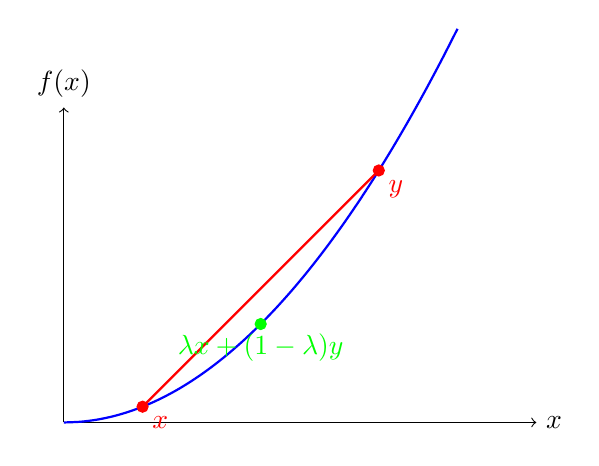
\begin{tikzpicture}
    \draw[->] (0,0) -- (6,0) node[right] {$x$};
    \draw[->] (0,0) -- (0,4) node[above] {$f(x)$};
    
    % Convex function
    \draw[blue, thick, domain=0:5, smooth, variable=\x] plot ({\x}, {0.2*\x*\x});
    
    % Two points
    \filldraw[red] (1,0.2) circle (2pt) node[below right] {$x$};
    \filldraw[red] (4,3.2) circle (2pt) node[below right] {$y$};
    
    % Line segment
    \draw[red, thick] (1,0.2) -- (4,3.2);
    
    % Midpoint
    \filldraw[green] (2.5,1.25) circle (2pt) node[below] {$\lambda x + (1-\lambda)y$};
    
    \end{tikzpicture}
    \caption{Example of a Convex Function}
    \label{fig:convex_function}
\end{figure}

\subsubsection{Convex Set}
A convex set means that the line segment connecting any two points in the set lies entirely within the set:
\begin{equation}
\lambda x + (1-\lambda)y \in S, \quad \forall x,y \in S, \forall \lambda \in [0,1]
\end{equation}

\begin{figure}[H]
    \centering
    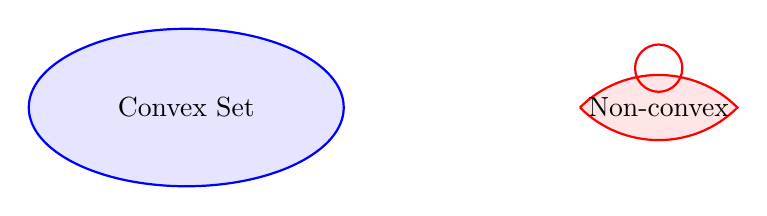
\begin{tikzpicture}
    % Convex set
    \draw[blue, thick, fill=blue!10] (0,0) ellipse (2 and 1);
    \node at (0,0) {Convex Set};
    
    % Non-convex set
    \draw[red, thick, fill=red!10] (5,0) to[out=45,in=135] (7,0) to[out=-135,in=-45] (5,0);
    \draw[red, thick] (6,0.5) circle (0.3);
    \node at (6,0) {Non-convex};
    \end{tikzpicture}
    \caption{Examples of Convex and Non-convex Sets}
    \label{fig:convex_nonconvex_sets}
\end{figure}

\subsubsection{Advantages of Convex Optimization}
Convex optimization holds special importance in optimization theory\sidenote{Effective algorithms and mathematical guarantees developed for convex optimization problems make solving these types of problems more reliable. The optimization problems within deep learning algorithms we frequently hear about today are generally convex optimization problems. The optimization algorithms used here are usually gradient descent methods. While they are very effective methods, they are generally inefficient in structural optimization problems.}:

\begin{itemize}
    \item \textbf{Local Optimum = Global Optimum:} A local minimum of a convex function is also the global minimum. This significantly simplifies the optimization process.
    \item \textbf{Stable Solution:} Regardless of the starting point, appropriate gradient-based algorithms converge to the same optimum point.
    \item \textbf{Efficient Algorithms:} Algorithms such as interior point methods and gradient descent can reach solutions in polynomial time for convex problems.
\end{itemize}

\begin{tcolorbox}[title=Example of Convex Optimization]
Quadratic programming problem:
\begin{equation}
\begin{aligned}
\min_{x \in \mathbb{R}^n} & \quad \frac{1}{2}x^TQx + c^Tx \\
\text{s.t.} & \quad Ax \leq b
\end{aligned}
\end{equation}

If $Q$ is a positive semi-definite matrix, this problem is convex and can be solved with efficient interior point methods.
\end{tcolorbox}

\subsubsection{Difficulties of Non-convex Optimization}
Non-convex optimization problems are frequently encountered challenges in structural optimization\sidenote{Most structural optimization problems are non-convex problems that can contain multiple local optima. This creates difficulties in finding the global optimum.}:

\begin{itemize}
    \item \textbf{Multiple Local Optima:} The function can contain multiple local minima, making it difficult to find the global optimum.
    \item \textbf{Starting Point Dependency:} Gradient-based algorithms can converge to different local optima depending on the starting point.
    \item \textbf{Computational Cost:} Generally, more comprehensive search methods are required to guarantee finding the global optimum, which increases computational cost.
\end{itemize}

\begin{tcolorbox}[title=Approaches to Non-convex Problems]
\begin{itemize}
    \item \textbf{Multiple Starting Points:} Multiple local optimizations are run from different starting points, and the best result is selected.
    \item \textbf{Metaheuristic Algorithms:} Methods such as genetic algorithms and particle swarm optimization try to approach the global optimum by exploring a wide solution space.
    \item \textbf{Convex Approximations:} The problem can be decomposed into convex sub-problems or solved using convex approximations (such as Sequential Convex Programming).
\end{itemize}
\end{tcolorbox}

\subsection{Constrained and Unconstrained Optimization}

\subsubsection{Unconstrained Optimization}
Unconstrained optimization, as the name suggests, refers to problems that do not contain any constraints, only requiring the minimization or maximization of the objective function. Mathematically:
\begin{equation}
\min_{x \in \mathbb{R}^n} f(x)
\end{equation}

\sidenote{Although unconstrained optimization is theoretically called "unconstrained," most engineering problems in practice contain physical or mathematical constraints in some way. The term "unconstrained" here means that there are no explicit constraints in the problem formulation.}

The main methods used to solve unconstrained optimization problems \sidenote{The principles of these five methods can be tested with Python code through the link:

\qrcode[height=1in]{https://github.com/btayfur/structural-optimization/blob/main/Code/Examples/Exmp2/}}:

\begin{itemize}
    \item \textbf{Gradient Descent Method:} Aims to reach the minimum by proceeding step by step in the direction of fastest decrease of the function (negative gradient direction). This method is widely used, especially in deep learning and machine learning applications.
    
    \item \textbf{Newton's Method:} Makes more intelligent decisions about both direction and step size by also using the function's second derivative (Hessian) information. Due to its quadratic convergence property, it converges faster than gradient descent under the right conditions.
    
    \item \textbf{Quasi-Newton Methods:} Methods that estimate the Hessian matrix approximately instead of calculating it directly to reduce the computational cost of Newton's method. BFGS and L-BFGS are among the most popular Quasi-Newton algorithms.
    
    \item \textbf{Conjugate Gradient Method:} A method that is particularly effective in large-scale problems and ensures that successive search directions are "conjugate" to each other.
    
    \item \textbf{Trust Region Methods:} Methods that determine a "trust region" in each iteration where the function can be locally well-modeled and search for the optimum within this region.
\end{itemize}

\begin{tcolorbox}[title=Mountain Climbing Analogy]
Let's think of a mountain climbing analogy to understand unconstrained optimization methods (for a maximization problem):

\begin{itemize}
    \item \textbf{Gradient Ascent:} You proceed in the steepest uphill direction at each step. Easy to implement but can progress slowly by zigzagging in narrow valleys.
    
    \item \textbf{Newton's Method:} You look not only at the slope of the ground (gradient) but also at the shape of the terrain (Hessian). This allows you to take large steps on flat areas and small, careful steps on steep slopes.
    
    \item \textbf{Quasi-Newton:} Instead of fully measuring the shape of the terrain, you estimate it from your previous steps. While not as effective as Newton, it requires much less effort.
\end{itemize}
\end{tcolorbox}

\subsubsection{Constrained Optimization}
Constrained optimization is much more common in modeling real-world problems and includes a set of constraints in addition to the objective function. These constraints represent the conditions that the solution must satisfy. Mathematical formulation:
\begin{equation}
\begin{aligned}
\min_{x \in \mathbb{R}^n} & \quad f(x) \\
\text{s.t.} & \quad g_i(x) \leq 0, \quad i = 1,\ldots,m \\
& \quad h_j(x) = 0, \quad j = 1,\ldots,p
\end{aligned}
\end{equation}

Here, $g_i(x) \leq 0$ represents inequality constraints, and $h_j(x) = 0$ represents equality constraints.

\sidenote{Structural optimization problems are almost always constrained problems. When you want to minimize the weight of a bridge, there are various constraints such as the bridge being able to carry certain loads, having a certain safety factor, and being constructible. An optimization without these constraints would not find practical application.}

The main methods used to solve constrained optimization problems:

\begin{itemize}
    \item \textbf{Lagrange Multipliers Method:} Defines additional variables called Lagrange multipliers for equality-constrained problems, transforming the constrained problem into an extended unconstrained problem. This method is particularly useful when constraints must be exactly satisfied.
    
    \item \textbf{Karush-Kuhn-Tucker (KKT) Conditions:} Optimality conditions valid for both equality and inequality constraints. KKT conditions are a generalization of the Lagrange multipliers method to inequality constraints.
    
    \item \textbf{Penalty Function Methods:} Transforms the constrained problem into an unconstrained problem by penalizing constraint violations. There are two main approaches:
    \begin{itemize}
        \item \textbf{Exterior Penalty Method:} Adds penalties for constraint violations, allows infeasible solutions but penalizes them.
        \item \textbf{Interior Penalty (Barrier) Method:} Adds an increasing penalty as the boundary of the feasible region is approached, ensuring the solution stays within the feasible region.
    \end{itemize}
    
    \item \textbf{Active Set Methods:} In each iteration, determines which constraints are believed to be active and solves a smaller subproblem. This is particularly effective in linear and quadratic programming problems.
    
    \item \textbf{Interior Point Methods:} Approaches the optimum while staying within the feasible region. Uses barrier functions but handles constraints directly. Very effective in large-scale linear and convex programming problems.
    
    \item \textbf{Sequential Quadratic Programming (SQP):} Solves constrained nonlinear problems by transforming them into a series of quadratic subproblems. Widely used in structural optimization.
\end{itemize}

\begin{tcolorbox}[title=Constrained Optimization Analogy: Path Finding]
You can think of constrained optimization as a path-finding problem where you have to follow certain rules while trying to find the best way to your destination:

\begin{itemize}
    \item \textbf{Your Goal (Objective Function):} To reach the mountain summit.
    \item \textbf{Your Constraints:} You can only walk on marked trails (equality constraints), you must stay away from certain dangerous areas (inequality constraints).
    
    \item \textbf{Lagrange Method:} Similar to continuously checking the trail map and dangerous areas while progressing.
    
    \item \textbf{Penalty Method:} If you leave the marked trail, you experience extra difficulty (getting stuck in mud, passing through thorny bushes, etc.). Despite these penalties, sometimes taking shortcuts can be advantageous.
    
    \item \textbf{Barrier Method:} You behave as if there's an invisible "repulsive force" around dangerous areas, retreating as you get closer. This way, you always stay in the safe region.
\end{itemize}
\end{tcolorbox}

\begin{tcolorbox}[title=Handling Constraints]
Methods to transform a constrained problem into an unconstrained problem:

\begin{itemize}
    \item \textbf{Exterior Penalty Method:} 
    \begin{equation}
    \min f(x) + c\sum\max(0,g_i(x))^2 + c\sum(h_j(x))^2
    \end{equation}
    
    Here $c > 0$ is the penalty parameter and is generally increased during iterations. As constraint violations increase, the penalty also increases, thus directing the algorithm toward the feasible region over time.
    
    \item \textbf{Interior Penalty (Barrier) Method:} 
    \begin{equation}
    \min f(x) - c\sum\ln(-g_i(x))
    \end{equation}
    
    This method is only defined when $g_i(x) < 0$ (i.e., within the feasible region) and as the constraint boundary is approached, $\ln(-g_i(x)) \to -\infty$, ensuring the solution stays within the feasible region. The $c$ parameter is generally decreased during iterations.
    
    \item \textbf{Augmented Lagrangian Method:} 
    \begin{equation}
    \min f(x) + \sum\lambda_j h_j(x) + \frac{c}{2}\sum(h_j(x))^2 + \sum\mu_i\max(0,g_i(x)) + \frac{c}{2}\sum\max(0,g_i(x))^2
    \end{equation}
    
    This method combines the advantages of Lagrange multipliers and penalty methods. Lagrange multipliers $\lambda_j$ and $\mu_i$ are updated in each iteration.
\end{itemize}
\end{tcolorbox}

\subsubsection{Comparison of Constrained and Unconstrained Optimization}

\begin{itemize}
    \item \textbf{Problem Difficulty:} Constrained problems are generally more difficult and require more specialized solution methods.
    
    \item \textbf{Solution Space:} In unconstrained problems, the entire search space can be used, while in constrained problems, the search is limited to the "feasible region."
    
    \item \textbf{Realism:} Real engineering problems are almost always constrained because designs must meet certain requirements.
    
    \item \textbf{Solution Strategy:} In solving constrained problems, the goal is generally to first satisfy the constraints, then optimize the objective function, or to handle these two goals in a balanced way.
\end{itemize}

\sidenote{Structural optimization problems generally contain quite complex constraints. For example, in the design of a skyscraper, while minimizing cost, many factors such as structural strength, user comfort, seismic performance, and wind loads must be considered as constraints. The nonlinearity of these constraints and their interaction with each other requires the development of special techniques to solve the problem.}

\subsection{Classification of Optimization Approaches}

\subsubsection{By Problem Structure}
Optimization problems can be categorized according to their mathematical structure, and this classification helps us determine which solution methods are appropriate:

\begin{itemize}
    \item \textbf{Linear Programming (LP)}
        \begin{itemize}
            \item Linear objective function: $f(x) = c^T x$
            \item Linear constraints: $Ax \leq b$, $Aeq \cdot x = beq$
            \item Basic solution methods: Simplex algorithm, Interior point methods
            \item Properties: Single global optimum, convex feasible region defined by constraints
            \item Application areas: Resource allocation, production planning, logistics optimization
        \end{itemize}
        
    \item \textbf{Nonlinear Programming (NLP)}
        \begin{itemize}
            \item Nonlinear objective function and/or constraints
            \item Subcategory - Convex Programming: Convex objective function, convex constraint set
            \item Subcategory - Non-convex Programming: Objective function and/or constraint set not convex
            \item Solution methods: Gradient-based methods (SQP, Interior point, BFGS), metaheuristic methods
            \item Application areas: Structural design, mechanical systems optimization, economic models
        \end{itemize}
        
    \item \textbf{Integer Programming (IP)}
        \begin{itemize}
            \item All variables must be integer: $x \in \mathbb{Z}^n$
            \item Subcategory - Mixed Integer Programming (MIP): Some variables integer, some continuous
            \item Subcategory - 0-1 Integer Programming: Variables can only take values 0 or 1
            \item Solution methods: Branch-and-bound, Cutting plane, Branch-and-cut
            \item Application areas: Scheduling problems, cutting/packing problems, topology optimization
        \end{itemize}
        
    \item \textbf{Stochastic Programming}
        \begin{itemize}
            \item Problems containing random variables
            \item Cases where uncertainty is modeled with probability distributions
            \item Solution methods: Scenario approach, sample average approximation, robust optimization
            \item Application areas: Risk management, portfolio optimization, structural design under uncertainty
        \end{itemize}
        
    \item \textbf{Multi-objective Programming}
        \begin{itemize}
            \item Simultaneous optimization of multiple objective functions
            \item Solution concept: Pareto-optimal solution set
            \item Solution methods: Weighted sum method, epsilon-constraint method, evolutionary algorithms like NSGA-II
            \item Application areas: Engineering design, environmental management, economic models
        \end{itemize}
\end{itemize}

\sidenote{A structural optimization problem generally carries characteristics of several of the above categories. For example, in a bridge design, section dimensions might be continuous variables while element types to be used might be integer variables. Additionally, material behavior might be expressed with nonlinear equations, and it might be necessary to optimize multiple criteria such as both cost and displacement. In this case, the problem becomes a mixed integer, nonlinear, multi-objective optimization problem.}

\subsubsection{By Solution Strategy}
Algorithms used to solve optimization problems can be categorized according to their search strategies:

\begin{itemize}
    \item \textbf{Deterministic Methods}
        \begin{itemize}
            \item \textbf{Gradient-based methods:} Progress in the direction of fastest improvement using derivative information of the function.
                \begin{itemize}
                    \item Advantages: Usually fast convergence, guaranteed reach to local optimum
                    \item Disadvantages: Getting stuck in local optima, derivative calculation requirement
                    \item Examples: Gradient descent, Newton, BFGS, Conjugate gradient
                \end{itemize}
                
            \item \textbf{Direct search methods:} Progress using function evaluations without derivative information.
                \begin{itemize}
                    \item Advantages: No derivatives required, suitable for noisy functions
                    \item Disadvantages: Usually slower convergence
                    \item Examples: Nelder-Mead simplex, Hooke-Jeeves pattern search
                \end{itemize}
                
            \item \textbf{Interior point methods:} Reach the optimum while staying within the feasible region.
                \begin{itemize}
                    \item Advantages: Effective in large-scale problems, polynomial time algorithm
                    \item Disadvantages: Complex implementation, starting point requirement
                    \item Examples: Primal-dual interior point, barrier methods
                \end{itemize}
        \end{itemize}
    
    \item \textbf{Stochastic/Metaheuristic Methods}
        \begin{itemize}
            \item \textbf{Evolutionary algorithms:} Mimic natural selection and genetic mechanisms.
                \begin{itemize}
                    \item Advantages: Potential to find global optimum, no derivatives required, suitable for parallel processing
                    \item Disadvantages: High computational cost, sensitive parameter tuning
                    \item Examples: Genetic algorithms, differential evolution, evolution strategies
                \end{itemize}
                
            \item \textbf{Swarm-based algorithms:} Search for solutions by modeling collective behaviors of animal groups.
                \begin{itemize}
                    \item Advantages: Easy implementation, effective in non-convex problems
                    \item Disadvantages: Weak theoretical guarantees, variable solution quality
                    \item Examples: Particle swarm optimization, ant colony optimization, bee algorithm
                \end{itemize}
                
            \item \textbf{Physics-based algorithms:} Perform optimization by mimicking physical processes.
                \begin{itemize}
                    \item Advantages: Ability to escape local optima
                    \item Disadvantages: Slow convergence, parameter sensitivity
                    \item Examples: Simulated annealing, harmony search, big bang-big crunch
                \end{itemize}
        \end{itemize}
    
    \item \textbf{Hybrid Methods} \sidenote{Hybrid methods combine the advantages of different approaches to provide more robust and effective solutions. For example, starting with a genetic algorithm for global search and then refining promising regions with a local gradient-based algorithm both increases the chance of finding the global optimum and ensures reaching a precise solution.}
        \begin{itemize}
            \item \textbf{Deterministic + Stochastic hybrid:} Combines advantages of both approaches.
                \begin{itemize}
                    \item Advantages: Combining global search with local optimization
                    \item Disadvantages: Complex implementation, difficult parameter tuning
                    \item Examples: Memetic algorithms, multi-start gradient methods
                \end{itemize}
                
            \item \textbf{Multi-level approaches:} Handles the problem at different detail levels.
                \begin{itemize}
                    \item Advantages: Ability to solve large and complex problems
                    \item Disadvantages: Problem-specific design requirement
                    \item Examples: Coarse-fine grid methods, hierarchical optimization
                \end{itemize}
                
            \item \textbf{Adaptive strategies:} Changes algorithm parameters or strategies during the optimization process.
                \begin{itemize}
                    \item Advantages: Dynamic adaptation to problem characteristics
                    \item Disadvantages: Complex control mechanisms
                    \item Examples: Adaptive metaheuristic methods, self-adaptive evolution strategies \sidenote{In structural optimization problems, since the computational cost of finite element analysis is generally high, algorithms that perform as few function evaluations as possible are preferred. Therefore, surrogate model-based optimization methods are becoming increasingly popular. These methods speed up the optimization process by using approximate models that can be calculated faster instead of real analysis.} 
                \end{itemize}
        \end{itemize}
\end{itemize}

\begin{tcolorbox}[title=Optimization Algorithm Selection]
Which algorithm is most suitable for an optimization problem depends on the problem's characteristics:

\begin{itemize}
    \item \textbf{Problem size:} Interior point methods, gradient-based methods, or specially designed metaheuristic methods are suitable for large-scale problems.
    
    \item \textbf{Derivative information:} If derivative calculation is possible and economical, gradient-based methods are generally faster. If derivative calculation is difficult or impossible, direct search or metaheuristic methods are preferred.
    
    \item \textbf{Problem nature:} Deterministic methods are generally sufficient for convex problems. Metaheuristic or hybrid methods are more suitable for non-convex, multimodal problems.
    
    \item \textbf{Computational budget:} If computational resources are limited, more efficient deterministic methods may be preferred. If high computational power is available, more comprehensive global search methods can be used.
    
    \item \textbf{Importance of feasible solution:} If feasible solutions are needed in intermediate iterations, methods that stay within the feasible region (interior point, barrier methods) may be preferred.
\end{itemize}
\end{tcolorbox}   
\section{Theoretical Foundations of Classical Optimization Algorithms}

Traditional optimization methods not only form the fundamental principles of modern algorithms but also remain among the most reliable tools for solving engineering problems. In this section, we will provide an in-depth look at the mathematical foundations of these methods and examine how they are applied to structural optimization problems.

\subsection{Analytical Foundations of Mathematical Optimization}

Optimization has been one of the most fundamental problems throughout mathematical history. Even before Leibniz and Newton developed differential calculus, mathematicians were dealing with optimization problems. In the modern sense, the analytical foundations of mathematical optimization are based on three fundamental concepts: stationarity, convexity, and duality.

\begin{tcolorbox}[title=Historical Perspective]
\begin{itemize}
    \item \textbf{Ancient Greece:} Euclidean geometry and maximum-minimum problems
    \item \textbf{17th Century:} Fermat, Leibniz, and Newton's differential calculus
    \item \textbf{18th Century:} Lagrange and Euler's variational calculations
    \item \textbf{19th Century:} Hamilton and Jacobi's optimization theories
    \item \textbf{20th Century:} Development of linear programming, numerical optimization, and complex algorithms
\end{itemize}
\end{tcolorbox}

\subsubsection{First and Second Order Optimality Conditions}

The most important analytical conditions that form the mathematical basis of optimization are:

\textbf{First Order Necessary Condition (Stationarity):} 
If $x^*$ is a local minimum, then $\nabla f(x^*) = 0$ must hold. This means that the gradient of the function is zero, i.e., the tangent plane is horizontal.

\textbf{Second Order Sufficient Condition:} 
If $\nabla f(x^*) = 0$ and the Hessian matrix $\nabla^2 f(x^*)$ is positive definite, then $x^*$ is a strict local minimum. Mathematically, for all $d \neq 0$, the condition $d^T \nabla^2 f(x^*) d > 0$ must be satisfied.

\sidenote{Second order conditions help us determine whether a critical point (where the gradient is zero) is a local minimum, local maximum, or a saddle point. In structural optimization problems, the evaluation of the Hessian matrix is critical for the algorithm's progress.}

\subsubsection{Special Case of Convex Optimization}

Convex optimization is a special case of classical optimization theory and has remarkable properties:

\begin{itemize}
    \item If the objective function and constraint set are convex, every local minimum is also a global minimum
    \item In convex problems, critical point conditions guarantee the global optimum
    \item In structural mechanics, potential energy minimization for linear elastic structures is a convex problem
    \item Even for non-convex problems, they can often be decomposed into convex subproblems
\end{itemize}

\begin{marginfigure}
\centering
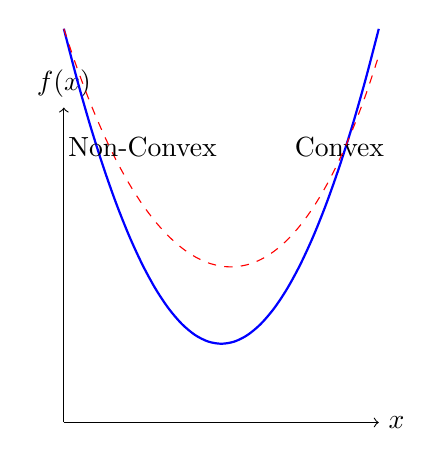
\begin{tikzpicture}
\draw[->] (0,0) -- (4,0) node[right] {$x$};
\draw[->] (0,0) -- (0,4) node[above] {$f(x)$};

% Convex and non-convex functions
\draw[scale=1,domain=0:4,smooth,variable=\x,blue,thick] plot ({\x},{(\x-2)^2+1});
\node at (3.5,3.5) {Convex};

\draw[scale=1,domain=0:4,smooth,variable=\x,red,dashed] plot ({\x},{sin(50*\x)+(\x-2)^2+1});
\node at (1,3.5) {Non-Convex};

\end{tikzpicture}
\caption{Comparison of convex and non-convex functions}
\label{fig:convexity}
\end{marginfigure}

\subsection{Gradient-Based Optimization Algorithms}

Gradient-based algorithms are methods that systematically approach the optimum point using derivative information of the function. These methods are of great importance in structural optimization problems in terms of computational efficiency and convergence properties.

\subsubsection{Gradient Descent Method and Its Variations}
The gradient descent method is the most basic and oldest gradient-based optimization method. This method aims to reach the minimum point by moving in the direction of the steepest descent of the function.

\begin{equation}
x_{k+1} = x_k - \alpha_k \nabla f(x_k)
\end{equation}

Here, $\alpha_k$ represents the step size (or learning rate) and significantly affects the algorithm's performance.

\begin{tcolorbox}[title=Gradient Descent Variations]
\begin{itemize}
    \item \textbf{Fixed Step Size:} The simplest approach uses a constant $\alpha$ for all iterations. However, it may be too low for fast convergence or too high for stability.
    
    \item \textbf{Line Search:} In each iteration, the value of $\alpha_k$ that minimizes $f(x_k - \alpha \nabla f(x_k))$ is found. This approach can be implemented with Armijo, Wolfe, or Goldstein conditions.
    
    \item \textbf{Momentum Gradient Descent:} Considers previous gradient values to reduce getting stuck in local minima:
    $$x_{k+1} = x_k - \alpha_k \nabla f(x_k) + \beta (x_k - x_{k-1})$$
    
    \item \textbf{Nesterov Accelerated Gradient:} An improved version of momentum gradient descent, it calculates the gradient not at the current position but at the point where momentum would take it.
\end{itemize}
\end{tcolorbox}

\sidenote{In structural optimization problems, the gradient descent method is typically used in the initial stages of large-scale problems. Although its convergence rate is low, its computational cost is low and it can provide a good starting point for complex problems.}

\begin{marginfigure}
\centering
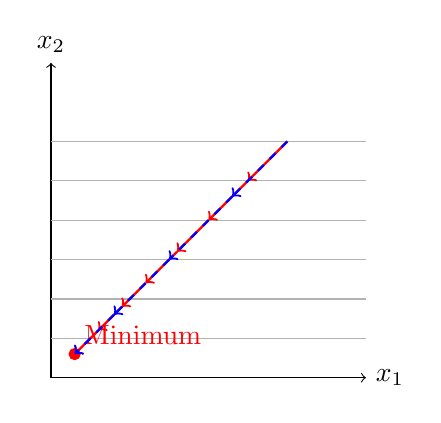
\begin{tikzpicture}
\draw[->] (0,0) -- (4,0) node[right] {$x_1$};
\draw[->] (0,0) -- (0,4) node[above] {$x_2$};

% Contour lines
\draw[scale=1,domain=0:4,smooth,variable=\x,black!30,thin] plot ({\x},{0.5});
\draw[scale=1,domain=0:4,smooth,variable=\x,black!30,thin] plot ({\x},{1.0});
\draw[scale=1,domain=0:4,smooth,variable=\x,black!30,thin] plot ({\x},{1.5});
\draw[scale=1,domain=0:4,smooth,variable=\x,black!30,thin] plot ({\x},{2.0});
\draw[scale=1,domain=0:4,smooth,variable=\x,black!30,thin] plot ({\x},{2.5});
\draw[scale=1,domain=0:4,smooth,variable=\x,black!30,thin] plot ({\x},{3.0});

% Gradient descent path
\draw[->,red,thick] (3,3) -- (2.5,2.5);
\draw[->,red,thick] (2.5,2.5) -- (2.0,2.0);
\draw[->,red,thick] (2.0,2.0) -- (1.6,1.6);
\draw[->,red,thick] (1.6,1.6) -- (1.2,1.2);
\draw[->,red,thick] (1.2,1.2) -- (0.9,0.9);
\draw[->,red,thick] (0.9,0.9) -- (0.6,0.6);
\draw[->,red,thick] (0.6,0.6) -- (0.3,0.3);
\filldraw[red] (0.3,0.3) circle (2pt) node[above right] {Minimum};

% Momentum gradient descent path
\draw[->,blue,thick,dashed] (3,3) -- (2.3,2.3);
\draw[->,blue,thick,dashed] (2.3,2.3) -- (1.5,1.5);
\draw[->,blue,thick,dashed] (1.5,1.5) -- (0.8,0.8);
\draw[->,blue,thick,dashed] (0.8,0.8) -- (0.3,0.3);

\end{tikzpicture}
\caption{Comparison of gradient descent (red, solid) and momentum gradient descent (blue, dashed) methods}
\label{fig:gradient_descent_variants}
\end{marginfigure}

\paragraph{Gradient Calculation in Structural Optimization}
In structural optimization problems, three methods are typically used for gradient calculation:

\begin{itemize}
    \item \textbf{Analytical Gradient:} Obtained through direct differential calculation. Provides the most accurate result but derivative derivation can be difficult in complex systems.
    
    \item \textbf{Finite Differences:} Gradient is calculated using numerical approximation:
    $$\frac{\partial f}{\partial x_i} \approx \frac{f(x + h e_i) - f(x)}{h}$$
    Easy to compute but the choice of $h$ is sensitive and computational cost is high for large systems.
    
    \item \textbf{Adjoint Method:} Particularly efficient for large-scale structural problems. Requires a constant number of system solutions independent of the number of design variables. Frequently used in finite element analysis.
\end{itemize}

\subsubsection{Newton and Quasi-Newton Methods}
The Newton method is one of the most powerful tools in classical optimization. It uses second-order derivative information (Hessian matrix) to create a local quadratic approximation of the function and moves directly toward the minimum point of this approximation.

\begin{equation}
x_{k+1} = x_k - [\nabla^2 f(x_k)]^{-1} \nabla f(x_k)
\end{equation}

The greatest advantage of the Newton method is its quadratic convergence rate; that is, as it approaches the optimum point, the error decreases approximately by the square in each iteration. However, calculating and inverting the Hessian matrix is computationally expensive, especially for high-dimensional problems.

\paragraph{Modified Newton Methods}
Various modifications have been developed to reduce computational cost and achieve better performance in cases where the Newton method might be unstable:

\begin{itemize}
    \item \textbf{Levenberg-Marquardt Algorithm:} Modifies the Hessian matrix to make it more stable:
    $$x_{k+1} = x_k - [\nabla^2 f(x_k) + \lambda I]^{-1} \nabla f(x_k)$$
    Here, $\lambda$ is a damping parameter that adjusts the algorithm's behavior.
    
    \item \textbf{Trust Region Newton Method:} Defines a "trust region" in each iteration where the Hessian matrix is valid and minimizes the quadratic model within this region. Particularly common in structural optimization.
\end{itemize}

\paragraph{Quasi-Newton Methods}
To eliminate the computational cost of calculating the full Hessian matrix, quasi-Newton methods iteratively update an approximation of the Hessian matrix. The most popular quasi-Newton methods are:

\begin{equation}
x_{k+1} = x_k - B_k^{-1} \nabla f(x_k)
\end{equation}

Here, $B_k$ is the approximation of the Hessian matrix at the $k$th iteration.

\begin{tcolorbox}[title=Basic Quasi-Newton Algorithms]
\begin{itemize}
    \item \textbf{BFGS (Broyden-Fletcher-Goldfarb-Shanno):} The most widely used quasi-Newton method. Maintains the positive definiteness of the Hessian approximation, which increases the algorithm's stability. Frequently preferred in structural optimization problems.
    
    \item \textbf{DFP (Davidon-Fletcher-Powell):} An older method than BFGS, but generally not as stable.
    
    \item \textbf{SR1 (Symmetric Rank-One):} Requires less computation but does not guarantee positive definiteness.
    
    \item \textbf{L-BFGS (Limited-memory BFGS):} A memory-optimized version of BFGS developed for very high-dimensional problems. Preferred in large-scale structural optimization problems, especially in topology optimization.
\end{itemize}
\end{tcolorbox}

\paragraph{Newton and Quasi-Newton Applications in Structural Optimization}
In structural engineering, Newton and quasi-Newton methods are frequently used in the following types of problems:

\begin{itemize}
    \item \textbf{Shape Optimization:} In optimizing the external geometry of structures, especially for aerodynamic performance or thermal behavior
    
    \item \textbf{Cross-Section Optimization:} In optimizing element cross-sections of truss and frame structures, especially in structures exhibiting nonlinear behavior
    
    \item \textbf{Parameter Calibration:} In calibrating finite element models with experimental data, determining material parameters
    
    \item \textbf{Multi-physics Optimization:} In complex engineering problems where structural, thermal, and fluid behaviors are optimized together
\end{itemize}

\begin{marginfigure}
\centering
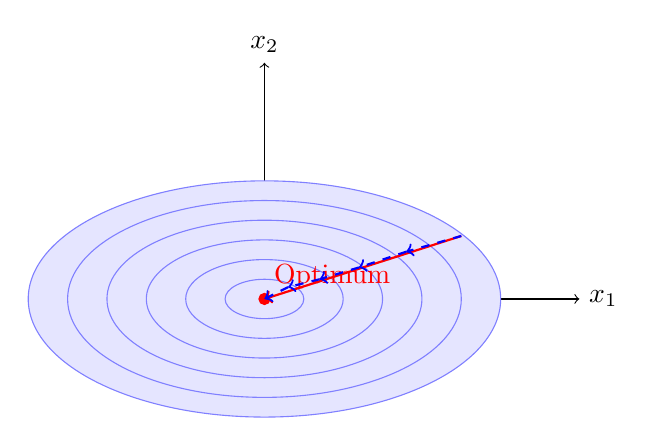
\begin{tikzpicture}
\draw[->] (0,0) -- (4,0) node[right] {$x_1$};
\draw[->] (0,0) -- (0,3) node[above] {$x_2$};

% Contour lines
\fill[blue!10] (0,0) ellipse (3 and 1.5);
\draw[blue!50] (0,0) ellipse (0.5 and 0.25);
\draw[blue!50] (0,0) ellipse (1 and 0.5);
\draw[blue!50] (0,0) ellipse (1.5 and 0.75);
\draw[blue!50] (0,0) ellipse (2 and 1);
\draw[blue!50] (0,0) ellipse (2.5 and 1.25);
\draw[blue!50] (0,0) ellipse (3 and 1.5);

% Newton path
\draw[->,red,thick] (2.5,0.8) -- (0,0);
\filldraw[red] (0,0) circle (2pt) node[above right] {Optimum};

% Gradient descent path
\draw[->,blue,thick,dashed] (2.5,0.8) -- (1.8,0.6);
\draw[->,blue,thick,dashed] (1.8,0.6) -- (1.2,0.4);
\draw[->,blue,thick,dashed] (1.2,0.4) -- (0.7,0.25);
\draw[->,blue,thick,dashed] (0.7,0.25) -- (0.3,0.15);
\draw[->,blue,thick,dashed] (0.3,0.15) -- (0,0);

\end{tikzpicture}
\caption{Comparison of Newton method (red, solid) and gradient descent method (blue, dashed). The Newton method can reach the optimum in a single step for quadratic functions.}
\label{fig:newton_vs_gradient}
\end{marginfigure}

\subsection{Constrained Optimization and Duality Theory}

Engineering problems rarely appear unconstrained. In structural design, there are many constraints such as stress limits, displacement boundaries, physical constraints, and resource limitations. In this section, we will examine in depth the classical approaches to solving constrained optimization problems.

\subsubsection{Lagrange Multipliers Method and Theoretical Foundations}

The Lagrange multipliers method is a fundamental approach developed for solving equality-constrained optimization problems. Developed by Joseph-Louis Lagrange in the 18th century, this method is one of the cornerstones of optimization theory and variational calculus.

An equality-constrained optimization problem is expressed as:
\begin{equation}
\begin{aligned}
\min & \quad f(x) \\
\text{s.t.} & \quad h_j(x) = 0, \quad j = 1, \ldots, p
\end{aligned}
\end{equation}

The Lagrange function (or Lagrangian) is defined as:
\begin{equation}
\mathcal{L}(x,\lambda) = f(x) + \sum_{j=1}^p \lambda_j h_j(x)
\end{equation}

Here, the $\lambda_j$ values are called Lagrange multipliers and represent the "shadow price" or marginal value of each constraint.

\sidenote{In structural engineering, Lagrange multipliers often have physical meaning. For example, in an optimization problem where we use force equilibrium as a constraint, the Lagrange multipliers typically correspond to displacements. This duality is a fundamental concept in finite element analysis and structural optimization.}

\paragraph{Lagrange Conditions}
The necessary conditions for a local minimum of a constrained optimization problem are:

\begin{equation}
\begin{aligned}
\nabla_x \mathcal{L}(x^*,\lambda^*) &= \nabla f(x^*) + \sum_{j=1}^p \lambda_j^* \nabla h_j(x^*) = 0 \\
\nabla_{\lambda} \mathcal{L}(x^*,\lambda^*) &= h_j(x^*) = 0, \quad j = 1, \ldots, p
\end{aligned}
\end{equation}

These conditions express that at the optimal point, the gradient of the objective function must be equal to a linear combination of the gradients of the constraint functions. Geometrically, this means that the level curves of $f(x)$ and $h_j(x)$ must be tangent.

\begin{figure}
\centering
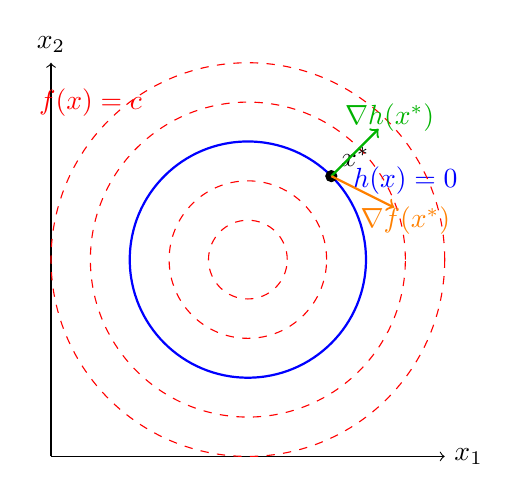
\begin{tikzpicture}
\draw[->] (0,0) -- (5,0) node[right] {$x_1$};
\draw[->] (0,0) -- (0,5) node[above] {$x_2$};

% Constraint function (a circle)
\draw[blue,thick] (2.5,2.5) circle (1.5);
\node[blue] at (4.5,3.5) {$h(x) = 0$};

% Objective function level curves
\draw[red,dashed] (2.5,2.5) circle (0.5);
\draw[red,dashed] (2.5,2.5) circle (1);
\draw[red,dashed] (2.5,2.5) circle (2);
\draw[red,dashed] (2.5,2.5) circle (2.5);
\node[red] at (0.5,4.5) {$f(x) = c$};

% Optimum point
\filldraw[black] (3.56,3.56) circle (2pt) node[above right] {$x^*$};

% Gradients
\draw[->,green!70!black,thick] (3.56,3.56) -- (4.16,4.16);
\node[green!70!black] at (4.3,4.3) {$\nabla h(x^*)$};

\draw[->,orange,thick] (3.56,3.56) -- (4.36,3.16);
\node[orange] at (4.5,3) {$\nabla f(x^*)$};

\end{tikzpicture}
\caption{Geometric interpretation of the Lagrange multipliers method: At the optimum point, the level curve of the objective function is tangent to the level curve of the constraint function.}
\label{fig:lagrange_geometry}
\end{figure}

\paragraph{Second Order Conditions}
To determine whether a critical point is actually a minimum, the extended Hessian matrix must be examined. If this matrix is positive definite in the tangent space of the constraints, the critical point is considered a local minimum.

\begin{tcolorbox}[title=Applications of Lagrange Method in Structural Optimization]
\begin{itemize}
    \item \textbf{Steel Frame Structures:} Ensuring force equilibrium at nodes and element compatibility while minimizing weight
    
    \item \textbf{Composite Material Design:} Ensuring volume constraint and material balance conditions while maximizing stiffness
    
    \item \textbf{Truss Systems:} Ensuring isostatic equilibrium conditions while minimizing weight
    
    \item \textbf{Finite Element Analysis:} Ensuring kinematic compatibility and force equilibrium constraints in finite element formulations based on energy minimization principle
\end{itemize}
\end{tcolorbox}

\subsubsection{Karush-Kuhn-Tucker (KKT) Conditions and Inequality Constraints}

The Karush-Kuhn-Tucker (KKT) conditions are a generalization of the Lagrange multipliers method for inequality-constrained problems. These conditions provide a fundamental framework for characterizing optimal solutions in the field of nonlinear programming.

An inequality-constrained optimization problem is expressed as:
\begin{equation}
\begin{aligned}
\min & \quad f(x) \\
\text{s.t.} & \quad g_i(x) \leq 0, \quad i = 1, \ldots, m \\
& \quad h_j(x) = 0, \quad j = 1, \ldots, p
\end{aligned}
\end{equation}

The Lagrange function in this case is:
\begin{equation}
\mathcal{L}(x,\lambda,\mu) = f(x) + \sum_{i=1}^m \mu_i g_i(x) + \sum_{j=1}^p \lambda_j h_j(x)
\end{equation}

\paragraph{KKT Conditions}
The necessary conditions for a local minimum of an inequality-constrained problem (KKT conditions) are:

\begin{equation}
\begin{aligned}
\nabla f(x^*) + \sum_{i=1}^m \mu_i^* \nabla g_i(x^*) + \sum_{j=1}^p \lambda_j^* \nabla h_j(x^*) &= 0 \\
g_i(x^*) &\leq 0, \quad i = 1, \ldots, m \\
h_j(x^*) &= 0, \quad j = 1, \ldots, p \\
\mu_i^* &\geq 0, \quad i = 1, \ldots, m \\
\mu_i^* g_i(x^*) &= 0, \quad i = 1, \ldots, m
\end{aligned}
\end{equation}

The last condition is known as "complementary slackness" and expresses that a constraint must either be active (satisfied as equality) or its corresponding Lagrange multiplier must be zero.

\begin{tcolorbox}[title=Interpretation of KKT Conditions]
\begin{itemize}
    \item \textbf{Stationarity:} The gradient of the objective function must be expressed as a linear combination of the gradients of active constraints. This shows that at the optimum point, progress is not possible without violating at least one active constraint.
    
    \item \textbf{Primal Feasibility:} All constraints must be satisfied.
    
    \item \textbf{Dual Feasibility:} The Lagrange multipliers (Kuhn-Tucker multipliers) for inequality constraints must be non-negative. This shows that the direction of constraints is important.
    
    \item \textbf{Complementary Slackness:} If any constraint is not active (satisfied as inequality), its corresponding Lagrange multiplier must be zero. This means the constraint is "inactive."
\end{itemize}
\end{tcolorbox}

\paragraph{Importance of KKT Conditions in Structural Optimization}
Structural optimization problems typically involve numerous inequality constraints. For example:
\begin{itemize}
    \item Stress constraints: $\sigma_i \leq \sigma_{allow}$
    \item Displacement constraints: $|u_i| \leq u_{allow}$
    \item Buckling constraints: $P_i \leq P_{cr,i}$
    \item Geometric constraints: minimum thickness, width, etc.
\end{itemize}

In such problems, KKT conditions provide not only a mathematical tool but also a framework with physical meaning. For example, the Lagrange multiplier associated with a stress constraint shows the effect of a unit stress increase at the relevant point on the weight of the optimal design. This is a fundamental concept for "design sensitivity analysis."

\begin{marginfigure}
\centering
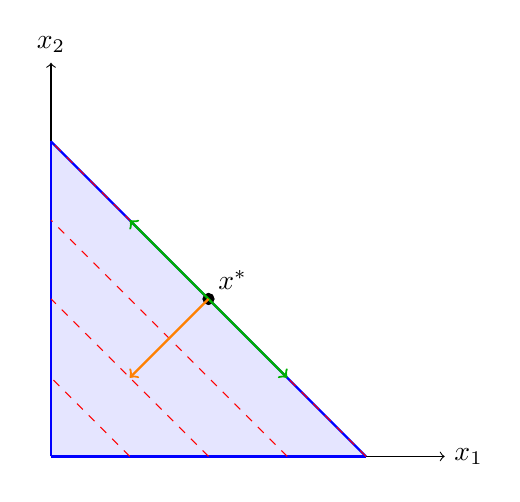
\begin{tikzpicture}
\draw[->] (0,0) -- (5,0) node[right] {$x_1$};
\draw[->] (0,0) -- (0,5) node[above] {$x_2$};

% Feasible region
\fill[blue!10] (0,0) -- (0,4) -- (2,2) -- (4,0) -- cycle;
\draw[blue,thick] (0,4) -- (2,2) -- (4,0);
\draw[blue,thick] (0,0) -- (0,4);
\draw[blue,thick] (0,0) -- (4,0);

% Objective function level lines
\draw[red,dashed] (1,0) -- (0,1);
\draw[red,dashed] (2,0) -- (0,2);
\draw[red,dashed] (3,0) -- (0,3);
\draw[red,dashed] (4,0) -- (0,4);

% Optimum point
\filldraw[black] (2,2) circle (2pt) node[above right] {$x^*$};

% Gradients of active constraints
\draw[->,green!70!black,thick] (2,2) -- (3,1);
\draw[->,green!70!black,thick] (2,2) -- (1,3);

% Objective function gradient
\draw[->,orange,thick] (2,2) -- (1,1);

\end{tikzpicture}
\caption{Geometric interpretation of KKT conditions: At the optimum point, the negative gradient of the objective function lies in the convex cone of the gradients of active constraints.}
\label{fig:kkt_geometry}
\end{marginfigure}

\paragraph{Duality Theory and Economic Interpretation}
Lagrange duality examines the relationship between the primal problem and its dual problem. The dual problem involves maximizing the Lagrange function instead of minimizing it:

\begin{equation}
\begin{aligned}
\max_{\mu \geq 0, \lambda} \min_{x} \mathcal{L}(x,\lambda,\mu)
\end{aligned}
\end{equation}

The duality theorem states that for a convex primal problem, the optimal value of the dual problem equals the optimal value of the primal problem (strong duality). This theorem forms the basis of many optimization algorithms.

From an economic perspective, dual variables (Lagrange multipliers) represent "shadow prices." In structural optimization, this shows the effect of a marginal change in a constraint on the value of the optimal design. This interpretation allows engineers to understand which constraints have the greatest impact on the design.

\begin{tcolorbox}[title=Relationship Between Duality and Structural Analysis]
In structural mechanics, the relationship between potential energy minimization (displacement method) and complementary energy minimization (force method) is a perfect example of the duality concept in optimization theory.

For the analysis of a structure:
\begin{itemize}
    \item \textbf{Primal Problem (Displacement Method):} Minimizing potential energy to find the compatible displacement field
    \item \textbf{Dual Problem (Force Method):} Minimizing complementary energy to find the force distribution in equilibrium
\end{itemize}

This duality is also used in the design of structural optimization algorithms. Particularly, "primal-dual" methods solve both the primal and dual problems simultaneously, providing more efficient optimization.
\end{tcolorbox}

\subsection{Linear and Quadratic Programming}

An important subset of classical optimization methods consists of linear and quadratic programming methods. These methods provide efficient solution algorithms specifically developed for optimization problems with certain structures.

\subsubsection{Linear Programming and Structural Applications}

Linear programming (LP) examines optimization problems where both the objective function and constraints are linear. Standard form:

\begin{equation}
\begin{aligned}
\min & \quad c^T x \\
\text{s.t.} & \quad Ax = b \\
& \quad x \geq 0
\end{aligned}
\end{equation}

Linear programming made significant progress in the 1940s with George Dantzig's development of the Simplex algorithm. Today, Interior Point Methods are also widely used for large-scale linear programming problems.

\paragraph{Simplex Method and Geometric Interpretation}
The Simplex method aims to find the optimal solution by systematically examining the corner points (extreme points) of the feasible region. The fundamental theorem of LP states that the optimal solution must be at a corner point of the feasible region (if the solution is not unique).

The steps of this method:
\begin{itemize}
    \item Find a feasible corner point for initialization
    \item Move to a neighboring corner point that improves the objective function value
    \item Continue until no better neighboring corner point can be found
\end{itemize}

\begin{tcolorbox}[title=LP Applications in Structural Engineering]
\begin{itemize}
    \item \textbf{Plastic Limit Analysis:} Determining the collapse load of structures, optimization of plastic hinge distribution
    
    \item \textbf{Minimum Weight Design of Truss Systems:} Optimization of element cross-sections under linear behavior and static load conditions
    
    \item \textbf{Structural Resource Allocation:} Resource distribution to maximize structural performance under limited material or budget conditions
    
    \item \textbf{Transportation Network Optimization:} Optimization of bridge and road system placement, modeling of traffic flow
\end{itemize}
\end{tcolorbox}

\paragraph{Plastic Limit Analysis Example}
Plastic limit analysis is one of the most important applications of linear programming in structural engineering. Static theorem (lower bound) formulation:
\begin{equation}
\begin{aligned}
\max & \quad \lambda \\
\text{s.t.} & \quad B^T q = \lambda F + F_0 \\
& \quad |q_i| \leq q_i^p, \quad i = 1, \ldots, n
\end{aligned}
\end{equation}

Where:
\begin{itemize}
    \item $\lambda$: load factor
    \item $q$: internal forces vector
    \item $B$: equilibrium matrix
    \item $F$: variable external load vector
    \item $F_0$: constant external load vector
    \item $q_i^p$: plastic limit capacity for element $i$
\end{itemize}

This formulation determines the maximum load factor that the structure can withstand without collapse.

\sidenote{Plastic limit analysis is particularly important in the design of steel structures. By determining the maximum load that the structure can withstand using its plastic deformation capacity beyond the elastic limit, it enables more economical designs.}

\begin{marginfigure}
\centering
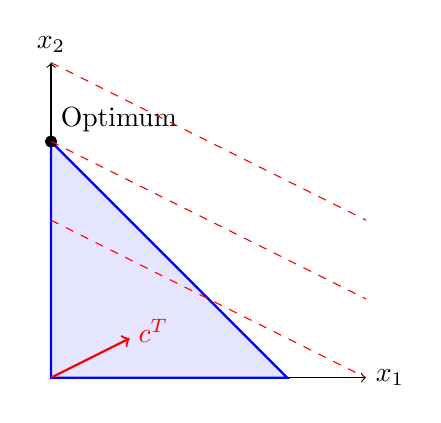
\begin{tikzpicture}
\draw[->] (0,0) -- (4,0) node[right] {$x_1$};
\draw[->] (0,0) -- (0,4) node[above] {$x_2$};

% Constraints and feasible region
\fill[blue!10] (0,0) -- (0,3) -- (1,2) -- (3,0) -- cycle;
\draw[blue,thick] (0,0) -- (0,3) -- (1,2) -- (3,0) -- cycle;

% Objective function vector
\draw[->,red,thick] (0,0) -- (1,0.5);
\node[red] at (1.3,0.6) {$c^T$};

% Optimum point
\filldraw[black] (0,3) circle (2pt) node[above right] {Optimum};

% Objective function level lines
\draw[red,dashed] (0,4) -- (4,2);
\draw[red,dashed] (0,3) -- (4,1);
\draw[red,dashed] (0,2) -- (4,0);

\end{tikzpicture}
\caption{Feasible region and optimum point in linear programming}
\label{fig:linear_programming}
\end{marginfigure}

\subsubsection{Quadratic Programming}

Quadratic programming (QP) deals with optimization problems where the objective function is quadratic and the constraints are linear:

\begin{equation}
\begin{aligned}
\min & \quad \frac{1}{2}x^TQx + c^Tx \\
\text{s.t.} & \quad Ax = b \\
& \quad x \geq 0
\end{aligned}
\end{equation}

Here, $Q$ is a symmetric matrix. If $Q$ is positive (semi) definite, the problem is convex and finding the global optimum is relatively easy.

\paragraph{Solution Methods}
Various solution methods have been developed for quadratic programming problems:
\begin{itemize}
    \item \textbf{Active Set Methods:} Solves unconstrained optimization subproblems by making predictions about which constraints are active
    
    \item \textbf{Interior Point Methods:} Approaches the optimum point by passing through the interior of the feasible region
    
    \item \textbf{Sequential Quadratic Programming (SQP):} Solves nonlinear optimization problems by dividing them into quadratic subproblems
\end{itemize}

\begin{tcolorbox}[title=QP Applications in Structural Engineering]
\begin{itemize}
    \item \textbf{Elastic Deformation Minimization:} Using the structure's stiffness matrix to minimize deformation under specific loads
    
    \item \textbf{Dynamic Behavior Optimization:} Using the structure's mass and stiffness matrices to optimize dynamic response
    
    \item \textbf{Finite Element Model Calibration:} Minimizing the squares of differences between experimental and numerical data
    
    \item \textbf{Weight and Displacement Optimization:} Multi-objective optimization involving both weight and displacement energy
\end{itemize}
\end{tcolorbox}

\paragraph{Structural Compliance Minimization Example}
A common quadratic programming problem in structural design is the minimization of compliance (or deformation energy) under a volume constraint:

\begin{equation}
\begin{aligned}
\min & \quad \frac{1}{2}F^Tu \\
\text{s.t.} & \quad Ku = F \\
& \quad \sum_{e=1}^{n_e} v_e\rho_e \leq V \\
& \quad 0 \leq \rho_e \leq 1, \quad e = 1, \ldots, n_e
\end{aligned}
\end{equation}

Where:
\begin{itemize}
    \item $u$: displacement vector
    \item $F$: force vector
    \item $K$: global stiffness matrix
    \item $\rho_e$: material density for element $e$ (design variable)
    \item $v_e$: volume of element $e$
    \item $V$: allowed total volume
\end{itemize}

This formulation forms the basis of topology optimization and is the starting point of the SIMP (Solid Isotropic Material with Penalization) method.

\subsection{Modern Classical Optimization Algorithms}

Modern extensions of classical optimization methods aim to solve large and complex structural optimization problems using various approaches. In this section, we will discuss more advanced versions of classical methods.

\subsubsection{Secant Methods and Structural Applications}

Secant methods are approaches developed to eliminate the requirement of calculating the Hessian matrix in the Newton method. These methods create an approximate estimate of the Hessian matrix using gradient information.

The most common secant methods are:
\begin{itemize}
    \item \textbf{Broyden Method:} Used in solving general nonlinear equation systems
    \item \textbf{DFP (Davidon-Fletcher-Powell) Method:} One of the first examples of quasi-Newton methods
    \item \textbf{BFGS (Broyden-Fletcher-Goldfarb-Shanno) Method:} Has become standard in many fields including structural optimization
\end{itemize}

In the BFGS method, the approximate value of the Hessian matrix is updated as follows:
\begin{equation}
B_{k+1} = B_k - \frac{B_k s_k s_k^T B_k}{s_k^T B_k s_k} + \frac{y_k y_k^T}{y_k^T s_k}
\end{equation}

Where:
\begin{itemize}
    \item $s_k = x_{k+1} - x_k$
    \item $y_k = \nabla f(x_{k+1}) - \nabla f(x_k)$
\end{itemize}

The BFGS method is widely used in structural optimization problems, especially when there are many design variables.

\paragraph{Advantages of BFGS in Structural Optimization}
\begin{itemize}
    \item \textbf{Memory Efficiency:} Applicable even to large-scale problems with the L-BFGS variant
    \item \textbf{Superlinear Convergence:} Convergence rate increases as it approaches the optimum point
    \item \textbf{Numerical Stability:} More stable than the Newton method
    \item \textbf{Integration with Line Search:} Can be combined with strong line search strategies
\end{itemize}

\subsubsection{Trust Region and Line Search Strategies}

The performance of gradient-based optimization methods depends largely on step size selection. Line search and trust region are two fundamental strategies developed for determining step size.

\paragraph{Line Search Strategies}
In line search methods, after determining the search direction $d_k$, a suitable step size $\alpha_k$ is found:
\begin{equation}
x_{k+1} = x_k + \alpha_k d_k
\end{equation}

Various criteria are used to determine the optimal step size:
\begin{itemize}
    \item \textbf{Armijo Condition:} Guarantees that the step size provides sufficient decrease in the function value
    \item \textbf{Wolfe Conditions:} In addition to the Armijo condition, requires that the gradient change satisfies a certain ratio
    \item \textbf{Goldstein Conditions:} Ensures both decrease in function value and that the step size is not too small
\end{itemize}

\paragraph{Trust Region Approach}
In trust region methods, a region where the model is reliable is defined and the model is minimized within this region:
\begin{equation}
\begin{aligned}
\min & \quad m_k(p) = f_k + g_k^Tp + \frac{1}{2}p^TB_kp \\
\text{s.t.} & \quad \|p\| \leq \Delta_k
\end{aligned}
\end{equation}

Where:
\begin{itemize}
    \item $m_k(p)$: quadratic model of the function at the $k$th iteration
    \item $f_k = f(x_k)$, $g_k = \nabla f(x_k)$
    \item $B_k$: Hessian matrix or its approximation
    \item $\Delta_k$: trust region radius
\end{itemize}

In each iteration, the trust region radius is updated by comparing the model prediction with the actual function change.

\begin{tcolorbox}[title=Trust Region Applications in Structural Engineering]
The trust region approach is particularly preferred in structural engineering in the following cases:
\begin{itemize}
    \item \textbf{Ill-Conditioned Problems:} When the condition number of the stiffness matrix is high
    
    \item \textbf{Nonlinear Behavior:} In structural analyses involving material or geometric nonlinearity
    
    \item \textbf{Unstable Systems:} In problems close to instability points such as buckling analysis
    
    \item \textbf{Multi-physics Analyses:} In complex multi-physics problems such as thermal-structural, fluid-structure interaction
\end{itemize}
\end{tcolorbox}

\subsubsection{Sequential Constraint Programming}

Sequential Constraint Programming (SCP) is an effective approach developed for solving structural optimization problems. This method solves the nonlinear problem by transforming it into a series of linear subproblems.

The basic approach of SCP:
\begin{itemize}
    \item Linearizes nonlinear constraints around the current iteration point
    \item Solves the linearized problem
    \item Uses the solution as a new iteration point
    \item Repeats until convergence
\end{itemize}

This method, with its more advanced variants such as MMA (Method of Moving Asymptotes), is widely used in structural topology optimization.

The main advantages of MMA in structural optimization:
\begin{itemize}
    \item Efficiency in large-scale topology optimization problems
    \item Effective handling of nonlinear constraints
    \item Stable convergence by reducing oscillations
    \item Suitability for parallel computing
\end{itemize}

\begin{figure}
\centering
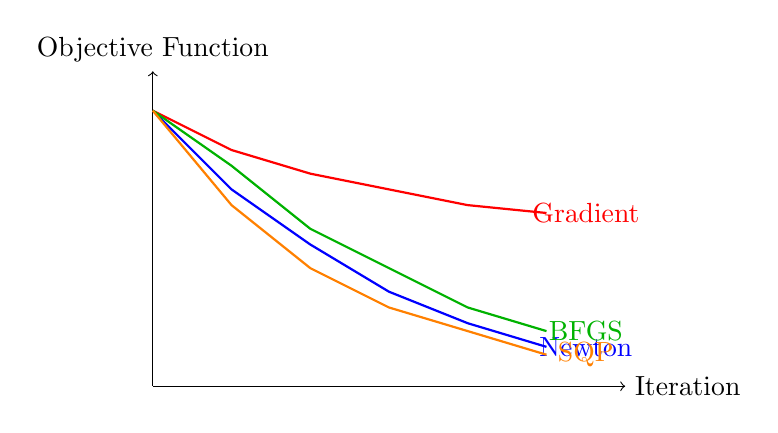
\begin{tikzpicture}
\draw[->] (0,0) -- (6,0) node[right] {Iteration};
\draw[->] (0,0) -- (0,4) node[above] {Objective Function};

% Gradient descent
\draw[red,thick] plot coordinates {(0,3.5) (1,3.0) (2,2.7) (3,2.5) (4,2.3) (5,2.2)};
\node[red] at (5.5,2.2) {Gradient};

% Newton
\draw[blue,thick] plot coordinates {(0,3.5) (1,2.5) (2,1.8) (3,1.2) (4,0.8) (5,0.5)};
\node[blue] at (5.5,0.5) {Newton};

% BFGS
\draw[green!70!black,thick] plot coordinates {(0,3.5) (1,2.8) (2,2.0) (3,1.5) (4,1.0) (5,0.7)};
\node[green!70!black] at (5.5,0.7) {BFGS};

% SQP
\draw[orange,thick] plot coordinates {(0,3.5) (1,2.3) (2,1.5) (3,1.0) (4,0.7) (5,0.4)};
\node[orange] at (5.5,0.4) {SQP};

\end{tikzpicture}
\caption{Comparison of convergence behaviors of different optimization algorithms}
\label{fig:convergence_comparison}
\end{figure}

\subsection{Conclusion and Transition to Modern Methods}

Classical optimization methods still hold great importance in solving various problems encountered in structural engineering. These methods form the foundation of modern meta-heuristic algorithms and artificial intelligence-based approaches.

\begin{tcolorbox}[title=Comparison of Classical and Modern Methods]
\begin{itemize}
    \item \textbf{Classical Methods:} Mathematical robustness, exact convergence guarantees, efficiency
    \item \textbf{Modern Methods:} Global search for multi-modal functions, parallel computing, flexibility in handling complex constraints
\end{itemize}
\end{tcolorbox}

Today, hybrid methods that combine the strengths of classical algorithms with the flexibility of modern approaches are receiving great interest. These hybrid approaches provide effective solutions, especially in large-scale and multi-objective structural optimization problems.
  
\section{Benchmark Test Fonksiyonları}
Bu başlık altında incelenen test fonksiyonlarına ait python kodlarına \href{https://github.com/btayfur/structural-optimization/blob/main/Code/Sources/OptimizationBenchmarks}{bağlantıdan} ulaşılabilir. \sidenote{
    
\qrcode[height=1in]{https://github.com/btayfur/structural-optimization/blob/main/Code/Sources/OptimizationBenchmarks}}

Optimizasyon algoritmalarının performansını değerlendirmek ve karşılaştırmak için kullanılan standart test fonksiyonları\sidenote{Test fonksiyonları, algoritmaların güçlü ve zayıf yönlerini ortaya çıkarmada önemli rol oynar. Bir algoritmanın gerçek dünya problemlerindeki başarısı, önce bu test fonksiyonları üzerinde değerlendirilir.}, farklı zorluk derecelerine sahip matematiksel yapılar olarak karşımıza çıkar. Bu test fonksiyonları, bilinen global minimum noktaları, karmaşık yerel minimum yapıları ve çeşitli topolojik özellikleri ile algoritmaları sınamak için tasarlanmıştır.

\subsection{Benchmark Fonksiyonlarının Optimizasyondaki Rolü}

Optimizasyon algoritmalarının performansını değerlendirmek için standart test fonksiyonları kullanılır. Bu fonksiyonlar şu açılardan önem taşır:

\begin{itemize}
    \item \textbf{Karşılaştırılabilirlik:} Farklı algoritmaların aynı problem üzerindeki başarısını objektif olarak değerlendirmeyi sağlar.
    \item \textbf{Güçlü ve Zayıf Yönleri Belirleme:} Algoritmaların hangi tür problemlerde iyi performans gösterdiğini, hangi tür problemlerde zorlandığını gösterir.
    \item \textbf{Algoritma Geliştirme:} Yeni optimizasyon algoritmalarının geliştirilmesi ve iyileştirilmesi sürecinde rehberlik eder.
    \item \textbf{Gerçek Dünya Uygulamalarına Hazırlık:} Algoritmaların daha karmaşık gerçek dünya problemlerine uygulanmadan önce test edilmesini sağlar.
\end{itemize}

İdeal bir benchmark fonksiyonu, gerçek dünyadaki optimizasyon problemlerinin karmaşıklığını yansıtırken, matematiksel olarak anlaşılabilir ve analiz edilebilir olmalıdır. Benchmark fonksiyonları genellikle şu özelliklere göre sınıflandırılır: doğrusallık, modalite (tepe nokta sayısı), süreklilik, türevlenebilirlik, sınırlılık ve boyutsallık.

\subsubsection{Benchmark Fonksiyonlarının Ortak Özellikleri}

Çoğu benchmark fonksiyonu aşağıdaki özelliklere sahiptir:

\begin{itemize}
    \item Bilinen global minimum değeri ve konumu
    \item Matematiksel olarak tanımlanmış yapı
    \item Ayarlanabilir boyut (genellikle çok boyutlu uzaylara genişletilebilir)
    \item Çeşitli zorluklar (örn. yerel minimumlar, düz bölgeler, dik vadiler)
    \item Önerilen arama aralıkları
\end{itemize}

\subsection{Çok Modlu ve Tek Modlu Test Fonksiyonları}

Test fonksiyonları, içerdikleri tepe noktası (mod) sayısına göre tek modlu (unimodal) ve çok modlu (multimodal) olarak ikiye ayrılır.

\subsubsection{Tek Modlu Fonksiyonlar}

Tek modlu fonksiyonlar, yalnızca bir tane global minimuma sahiptir ve genellikle daha basit yapıdadır. Bu fonksiyonlar, algoritmanın yakınsama hızını ve hassasiyetini test etmek için kullanılır. Örnek olarak:

\begin{itemize}
    \item \textbf{Sphere Fonksiyonu:} Matematiksel olarak en basit optimizasyon test fonksiyonudur ve şu şekilde tanımlanır:
    \begin{equation}
        f(\mathbf{x}) = \sum_{i=1}^{n} x_i^2
    \end{equation}
    Global minimum $f(\mathbf{x}^*) = 0$, $\mathbf{x}^* = (0, 0, \ldots, 0)$ noktasında yer alır.
    
    \item \textbf{Booth Fonksiyonu:} İki boyutlu, çanak şeklinde bir fonksiyondur:
    \begin{equation}
        f(x, y) = (x + 2y - 7)^2 + (2x + y - 5)^2
    \end{equation}
    Global minimum $f(1, 3) = 0$ noktasındadır.
\end{itemize}

\subsubsection{Çok Modlu Fonksiyonlar}

Çok modlu fonksiyonlar, birden fazla yerel minimuma sahiptir ve bu nedenle algoritmaların yerel minimumlara takılmadan global minimumu bulabilme yeteneğini test eder. Bu fonksiyonlar, özellikle metasezgisel ve evrimsel algoritmaların performansını değerlendirmek için önemlidir. Önemli örnekler arasında:

\begin{itemize}
    \item \textbf{Ackley Fonksiyonu:} Çok sayıda yerel minimumu olan karmaşık bir test fonksiyonudur. Matematiksel olarak şöyle tanımlanır:
    \begin{equation}
        f(\mathbf{x}) = -20\exp\left(-0.2\sqrt{\frac{1}{n}\sum_{i=1}^{n}x_i^2}\right) - \exp\left(\frac{1}{n}\sum_{i=1}^{n}\cos(2\pi x_i)\right) + 20 + e
    \end{equation}
    
    Bu fonksiyonun global minimumu $f(\mathbf{x}^*) = 0$, $\mathbf{x}^* = (0, 0, \ldots, 0)$ noktasında bulunur. Genellikle $[-32.768, 32.768]$ aralığında tanımlanır.
    
    \item \textbf{Rastrigin Fonksiyonu:} Sinüzoidal modülasyonu ile çok sayıda yerel minimuma sahip zorlayıcı bir fonksiyondur:
    \begin{equation}
        f(\mathbf{x}) = 10n + \sum_{i=1}^{n} \left[ x_i^2 - 10\cos(2\pi x_i) \right]
    \end{equation}
    Global minimum $f(\mathbf{x}^*) = 0$, $\mathbf{x}^* = (0, 0, \ldots, 0)$ noktasındadır.
\end{itemize}

\begin{figure}[h]
    \centering
    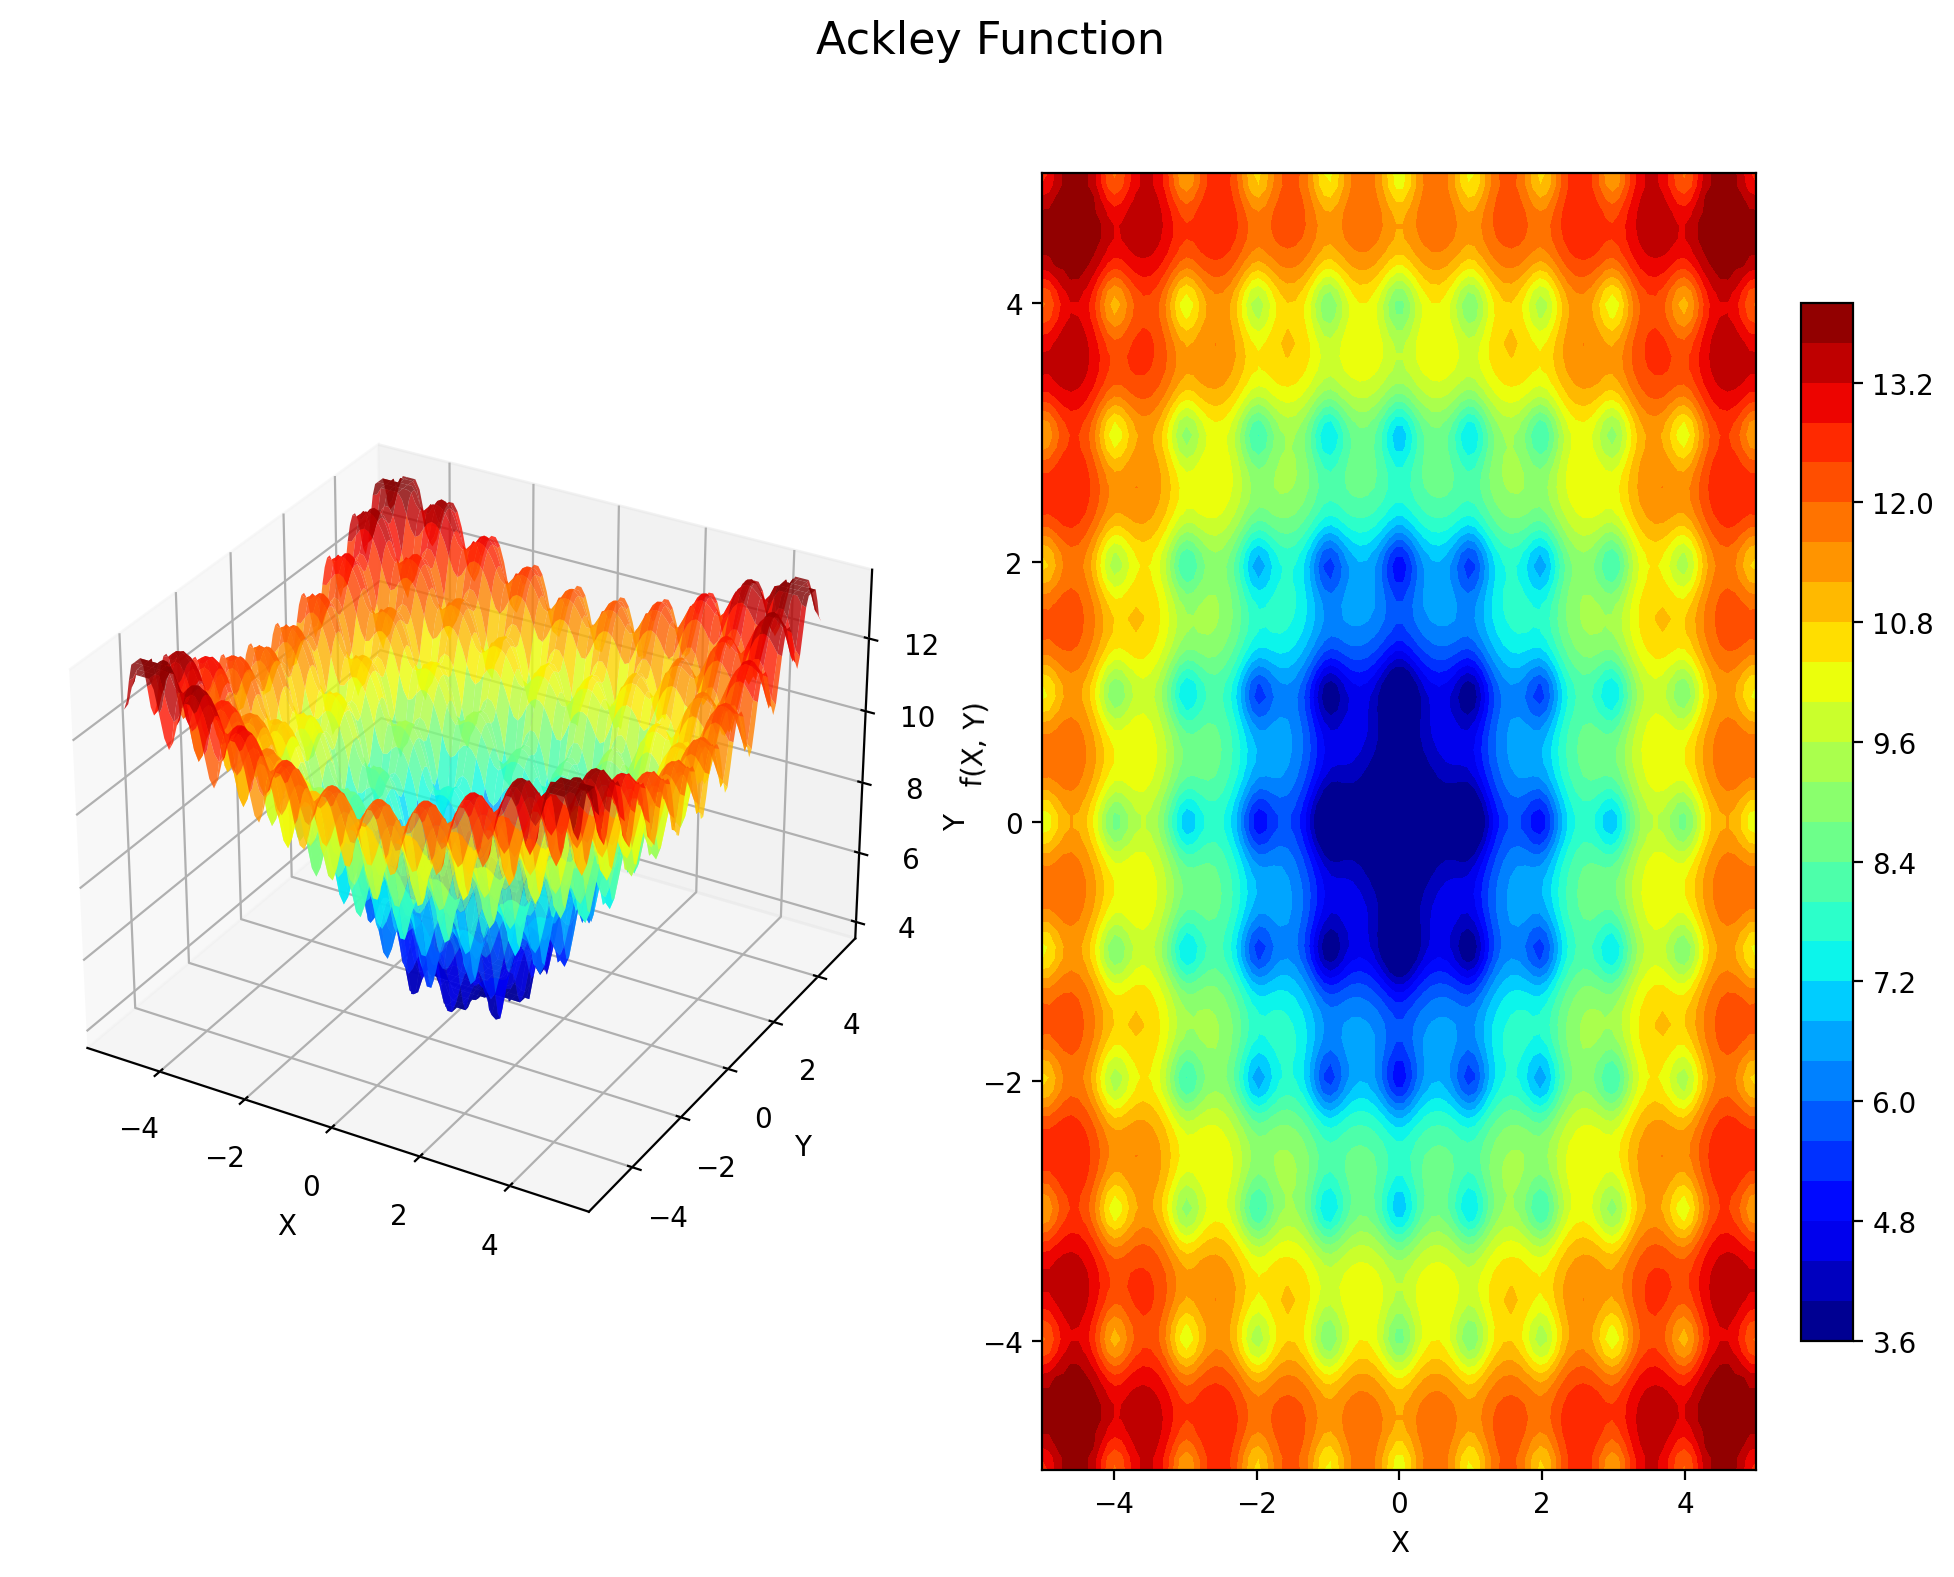
\includegraphics[width=0.8\textwidth]{weeks_new/imgs/ackley_function.png}
    \caption{Ackley fonksiyonunun 3B gösterimi (soldaki) ve kontur grafiği (sağdaki). Fonksiyonun merkezde bir global minimum ve etrafında çok sayıda yerel minimum içeren yapısı dikkat çekicidir.}
    \label{fig:ackley}
\end{figure}

\subsubsection{Ackley Fonksiyonu: Derinlemesine İnceleme}

Ackley fonksiyonu, David Ackley tarafından 1987 yılında önerilmiş ve optimizasyon algoritmaları için standart bir test fonksiyonu haline gelmiştir. Fonksiyonun matematiksel yapısı şu özellikleri ortaya çıkarır:

\begin{itemize}
    \item \textbf{Neredeyse düz bölgeler:} Merkezden uzaklaştıkça fonksiyon neredeyse düz bir yapıya sahiptir, bu da gradyan tabanlı yöntemlerin doğru yönü belirlemesini zorlaştırır.
    
    \item \textbf{Periyodik dalgalanmalar:} Kosinüs terimi nedeniyle, fonksiyon yüzeyi düzenli aralıklarla iniş ve çıkışlar gösterir, çok sayıda yerel minimum oluşturur.
    
    \item \textbf{Merkezdeki derin çukur:} Global minimum etrafında dik bir çukur bulunur, bu da algoritmanın optimuma yakın olduğunda hassas adımlar atmasını gerektirir.
\end{itemize}

Ackley fonksiyonu, özellikle şu tür algoritmaların test edilmesinde etkilidir:

\begin{itemize}
    \item Yerel aramayla global arama stratejilerini dengeleyen metasezgisel algoritmalar
    \item Çok sayıda yerel minimumdan kaçabilme yeteneğine sahip algoritmalar
    \item Farklı çözüm bölgelerini aynı anda keşfedebilen popülasyon tabanlı algoritmalar
\end{itemize}

$n$-boyutlu Ackley fonksiyonunun optimizasyonu şu zorlukları içerir:
\begin{itemize}
    \item Boyut arttıkça yerel minimum sayısı üstel olarak artar
    \item Merkeze yakın bölgelerde yüksek hassasiyet gerektirir
    \item Düz bölgelerde gradyan bilgisi yetersiz kalır
\end{itemize}

\begin{tcolorbox}[title=Ackley Fonksiyonu Optimizasyon Zorluğu]
Ackley fonksiyonu, hem keşif (exploration) hem de yararlanma (exploitation) özelliklerini aynı anda test eder:
\begin{itemize}
    \item Keşif: Geniş, neredeyse düz bölgelerde doğru yönü bulabilme
    \item Yararlanma: Merkezdeki dik çukurda hassas ayarlamaları yapabilme
    \item Denge: Yerel minimumlardan kaçarken global minimuma yakınsayabilme
\end{itemize}
\end{tcolorbox}

\subsection{Yüksek Boyutlu Optimizasyon Problemleri}

\subsubsection{Boyut Artışının Etkileri}
\begin{itemize}
    \item Arama uzayı üstel olarak büyür
    \item Hesaplama maliyeti artar
    \item Lokal minimum sayısı artar
    \item Yakınsama zorlaşır
\end{itemize}

Yüksek boyutlu optimizasyon problemleri, gerçek dünyadaki birçok mühendislik uygulamasında karşımıza çıkar. Boyut artışı, "boyutun laneti" (curse of dimensionality) olarak bilinen fenomene yol açar. Bu fenomen, boyut arttıkça arama uzayının üstel olarak büyümesi ve algoritmaların etkinliğinin dramatik biçimde azalması ile karakterize edilir.

\subsubsection{Boyutun Lanetinin Etkileri}

Boyut artışının optimizasyon süreci üzerindeki etkileri:

\begin{itemize}
    \item \textbf{Arama uzayı genişliği:} $n$ boyutlu ve her boyutta $m$ ayrık nokta içeren bir problemde, toplam arama uzayı $m^n$ büyüklüğündedir. Örneğin, her boyutta 10 nokta için, 2 boyutlu problemde 100 nokta, 10 boyutlu problemde $10^{10}$ nokta, 100 boyutlu problemde $10^{100}$ nokta vardır.
    
    \item \textbf{Veri seyrekliği:} Yüksek boyutlarda, veri noktaları arasındaki mesafeler artar ve veri seyrekleşir. Bu, algoritmaların doğru yönü belirlemesini zorlaştırır.
    
    \item \textbf{Örnekleme zorluğu:} Yüksek boyutlu uzayı yeterince örneklemek için gereken nokta sayısı, pratikte ulaşılamayacak kadar büyüktür.
\end{itemize}

\subsubsection{Yüksek Boyutlu Test Fonksiyonları}

Bazı test fonksiyonları özellikle yüksek boyutlu problemlerde algoritmaların performansını değerlendirmek için tasarlanmıştır:

\begin{itemize}
    \item \textbf{Rosenbrock Fonksiyonu:} Dar bir vadi boyunca ilerleyen ve boyut arttıkça zorlaşan bir fonksiyondur:
    \begin{equation}
        f(\mathbf{x}) = \sum_{i=1}^{n-1} \left[ 100(x_{i+1} - x_i^2)^2 + (x_i - 1)^2 \right]
    \end{equation}
    
    \item \textbf{Schwefel Fonksiyonu:} Yüksek boyutlarda çok sayıda geniş bölgeli yerel minimuma sahiptir:
    \begin{equation}
        f(\mathbf{x}) = 418.9829n - \sum_{i=1}^{n} x_i\sin(\sqrt{|x_i|})
    \end{equation}
\end{itemize}

\subsection{Stokastik Algoritmaların Test Edilmesi}

Stokastik algoritmalar, deterministik olmayan, rastgele elemanlara sahip algoritmalardır. Bu algoritmalar her çalıştırıldıklarında farklı sonuçlar üretebilirler. Metasezgisel algoritmalar, evrimsel algoritmalar ve yapay sinir ağları gibi modern optimizasyon yöntemleri genellikle stokastik karaktere sahiptir.

\subsubsection{Stokastik Algoritmaların Test Prensipleri}

\begin{itemize}
    \item \textbf{Çoklu çalıştırma:} Her test fonksiyonu için algoritma birden çok kez (genellikle 30-50 bağımsız çalıştırma) çalıştırılmalıdır.
    
    \item \textbf{İstatistiksel analiz:} Sonuçların ortalaması, standart sapması, medyanı, en iyi ve en kötü değerleri raporlanmalıdır.
    
    \item \textbf{Yakınsama analizi:} Algoritmanın zaman içindeki davranışı, iterasyon/değerlendirme sayısına karşı en iyi değer grafiği ile gösterilmelidir.
    
    \item \textbf{Parametre duyarlılığı:} Algoritmanın parametre değişimlerine olan duyarlılığı test edilmelidir.
\end{itemize}

\subsection{Test Prensipleri}

Optimizasyon algoritmalarının adil ve kapsamlı bir şekilde değerlendirilmesi için bazı temel prensiplere uyulmalıdır:

\begin{itemize}
    \item \textbf{Çeşitlilik:} Farklı özelliklere sahip test fonksiyonları kullanılmalıdır.
    
    \item \textbf{Adil karşılaştırma:} Karşılaştırılan tüm algoritmalar için aynı koşullar (başlangıç noktaları, fonksiyon değerlendirme sayısı, sonlandırma kriterleri) sağlanmalıdır.
    
    \item \textbf{Yeterli tekrar:} Stokastik algoritmalar için yeterli sayıda bağımsız çalıştırma yapılmalıdır.
    
    \item \textbf{Boyut değişimi:} Algoritmaların farklı problem boyutlarındaki performansı test edilmelidir.
    
    \item \textbf{Kapsamlı raporlama:} Sadece ortalama veya en iyi değerler değil, tam istatistiksel sonuçlar raporlanmalıdır.
\end{itemize}

\subsection{Performans Ölçütleri}

Optimizasyon algoritmalarının performansı çeşitli ölçütlerle değerlendirilebilir. Bu ölçütler, sayısal ve kalite olmak üzere iki ana kategoriye ayrılabilir.

\subsubsection{Sayısal Ölçütler}

\begin{itemize}
    \item \textbf{Yakınsama hızı:} Algoritmanın istenen çözüme ne kadar hızlı ulaştığını gösterir. Genellikle fonksiyon değerlendirme sayısı veya iterasyon sayısı olarak ölçülür.
    
    \item \textbf{Hassasiyet:} Bulunan çözümün bilinen global optimuma ne kadar yakın olduğunu gösterir. Genellikle mutlak veya göreceli hata olarak ölçülür.
    
    \item \textbf{Başarı oranı:} Algoritmanın kabul edilebilir bir çözüme ulaşma yüzdesidir. Özellikle stokastik algoritmalar için önemlidir.
    
    \item \textbf{Hesaplama karmaşıklığı:} Algoritmanın çalışma süresi veya bellek kullanımı olarak ölçülebilir.
\end{itemize}

\subsubsection{Kalite Ölçütleri}

\begin{itemize}
    \item \textbf{Sağlamlık (robustness):} Algoritmanın farklı problem tiplerine, başlangıç koşullarına ve parametre değişimlerine karşı duyarlılığı.
    
    \item \textbf{Genellenebilirlik:} Algoritmanın farklı problem sınıflarında gösterdiği performans.
    
    \item \textbf{Ölçeklenebilirlik:} Problem boyutu arttıkça algoritmanın performansındaki değişim.
    
    \item \textbf{Keşif-yararlanma dengesi:} Algoritmanın global arama (keşif) ve yerel iyileştirme (yararlanma) arasındaki dengeyi sağlama yeteneği.
\end{itemize}

\sidenote{Performans ölçütleri, farklı algoritmaların objektif olarak karşılaştırılmasını sağlar. Ancak, tek bir ölçüt yerine birden fazla ölçütün birlikte değerlendirilmesi daha sağlıklıdır.}

\begin{tcolorbox}[title=No Free Lunch Teoremi]
Hiçbir optimizasyon algoritması tüm problemlerde en iyi performansı gösteremez:
\begin{itemize}
    \item Her algoritmanın güçlü ve zayıf yönleri vardır
    \item Problem yapısına uygun algoritma seçimi önemlidir
    \item Hibrit yaklaşımlar avantajlı olabilir
\end{itemize}
\end{tcolorbox}

\subsubsection{Benchmark Sonuçlarının Sunumu}

Benchmark test sonuçlarının etkili sunumu için şu yöntemler kullanılabilir:

\begin{itemize}
    \item \textbf{Tablo formatı:} Algoritmaların her test fonksiyonu için ortalama, standart sapma, en iyi ve en kötü değerlerini gösteren tablolar.
    
    \item \textbf{Yakınsama grafikleri:} İterasyon/değerlendirme sayısına karşı en iyi değerin değişimini gösteren grafikler.
    
    \item \textbf{Kutu grafikleri (Box plots):} Sonuçların dağılımını ve medyan, çeyrekler gibi istatistiksel özetleri görsel olarak sunan grafikler.
    
    \item \textbf{Sıralama tabloları:} Algoritmaların her bir test fonksiyonu için performans sıralamasını gösteren tablolar.
    
    \item \textbf{İstatistiksel anlamlılık testleri:} Algoritmaların performans farklarının istatistiksel olarak anlamlı olup olmadığını gösteren testler (t-testi, Wilcoxon işaretli sıra testi, Friedman testi vb.).
\end{itemize}

\subsection{Benchmark Fonksiyonlarının Kategorileri}

Farklı özelliklere sahip benchmark fonksiyonları, algoritmaların çeşitli zorluklarla başa çıkma yeteneğini test eder. Burada, temel fonksiyon kategorileri ve örnekleri verilmiştir:

\subsubsection{Çok Sayıda Yerel Minimuma Sahip Fonksiyonlar}

Bu fonksiyonlar, algoritmalar için bir zorluk oluşturan birçok yerel minimuma sahiptir ve global optimizasyon yeteneğini test eder:

\begin{itemize}
    \item Ackley
    \item Rastrigin
    \item Griewank
    \item Schwefel
    \item Levy
    \item Shubert
\end{itemize}

\subsubsection{Çanak Şeklindeki Fonksiyonlar}

Bu fonksiyonlar, dairesel veya eliptik konturlarla çevrili tek bir minimuma sahiptir ve yerel optimizasyon yeteneğini test eder:

\begin{itemize}
    \item Sphere
    \item Bohachevsky
    \item Sum Squares
    \item Rotated Hyper-Ellipsoid
\end{itemize}

\subsubsection{Tabak Şeklindeki Fonksiyonlar}

Bu fonksiyonlar, algoritmaların doğru yönü belirleme yeteneğini zorlayabilen düz bölgelere sahiptir:

\begin{itemize}
    \item Booth
    \item Matyas
    \item Zakharov
    \item McCormick
\end{itemize}

\subsubsection{Vadi Şeklindeki Fonksiyonlar}

Bu fonksiyonlar, birçok algoritmanın yakınsamasını yavaşlatabilen uzun, dar vadilere sahiptir:

\begin{itemize}
    \item Rosenbrock (Muz Fonksiyonu)
    \item Six-Hump Camel
    \item Three-Hump Camel
    \item Dixon-Price
\end{itemize}

\subsubsection{Dik Sırtlar/Düşüşler İçeren Fonksiyonlar}

Bu fonksiyonlar, gradyan tabanlı yöntemleri zorlayabilecek dik sırtlara veya düşüşlere sahiptir:

\begin{itemize}
    \item Easom
    \item Michalewicz
    \item De Jong N.5
\end{itemize}

\subsection{Sonuç ve Uygulamalar}

Benchmark test fonksiyonları, optimizasyon algoritmalarının geliştirilmesi, test edilmesi ve karşılaştırılması için vazgeçilmez araçlardır. Bu fonksiyonlar, algoritmaların farklı problem tiplerindeki performansını değerlendirmeye ve zayıf yönlerini belirlemeye yardımcı olur.

\begin{itemize}
    \item \textbf{Algoritma geliştirmede:} Yeni algoritmaların güçlü ve zayıf yönlerinin belirlenmesi
    \item \textbf{Parametre ayarlamada:} Algoritma parametrelerinin optimizasyonu
    \item \textbf{Hibrit yaklaşımlarda:} Farklı algoritmaların güçlü yönlerini birleştiren hibrit yöntemlerin geliştirilmesi
    \item \textbf{Eğitimde:} Optimizasyon algoritmalarının davranışlarının anlaşılması
    \item \textbf{Gerçek dünya problemlerine hazırlıkta:} Daha karmaşık problemlere geçmeden önce algoritmaların temel yeteneklerinin değerlendirilmesi
\end{itemize}

  
\section{Metaheuristic Optimization Algorithms I}
Nature-inspired modern algorithms used in solving complex optimization problems will be discussed in this section. These algorithms provide effective solutions when classical methods prove insufficient.

\subsection{Basic Characteristics of Metaheuristic Algorithms}

Metaheuristic algorithms are nature-inspired methods used in solving complex optimization problems:

\begin{itemize}
    \item Have stochastic characteristics
    \item Problem-independent structure
    \item Do not require gradient information
    \item Potential to reach global optimum
\end{itemize}

\sidenote{The most important characteristic of metaheuristic algorithms is their potential to reach the global optimum without getting stuck in local optima in complex and multimodal problems.}

\subsection{Differences Between Deterministic and Stochastic Algorithms}

\begin{tcolorbox}[title=Deterministic vs Stochastic]
\begin{itemize}
    \item \textbf{Deterministic:}
        \begin{itemize}
            \item Same starting point → Same result
            \item Gradient-based
            \item Fast convergence to local optimum
        \end{itemize}
    \item \textbf{Stochastic:}
        \begin{itemize}
            \item Random search
            \item Different result in each run
            \item Global optimum potential
        \end{itemize}
\end{itemize}
\end{tcolorbox}

\subsection{Classification of Metaheuristic Algorithms Based on Search Method}

Metaheuristic algorithms are fundamentally divided into two categories based on search methods: population-based and single-solution search algorithms. Population-based algorithms evaluate multiple solution candidates simultaneously, while single-solution search algorithms work on a single solution. This classification provides an important framework for understanding the working principles and optimization strategies of algorithms.\sidenote{
This context can be examined through the link to better understand the working principles of algorithms.    

\qrcode[height=1in]{https://github.com/btayfur/structural-optimization/blob/main/Code/Examples/Exmp3}}

\subsubsection{Population-Based Algorithms}

Population-based algorithms are methods that evaluate multiple solution candidates simultaneously during the optimization process and benefit from interactions between these solutions. These algorithms increase the probability of reaching the global optimum by exploring different regions of the search space simultaneously. Population-based approaches reduce the risk of getting stuck in local optima by maintaining the diversity of solution candidates and provide effective results in complex, multimodal problems.

The most common examples of population-based algorithms include Genetic Algorithms, Particle Swarm Optimization, and Differential Evolution. In these algorithms, each individual (solution candidate) in the population evolves according to specific rules and interacts with others. For example, Genetic Algorithms use crossover and mutation operators, while in Particle Swarm Optimization, particles move by benefiting from their own experience and the collective knowledge of the swarm. These interactions ensure that the algorithm uses both exploration and exploitation capabilities in a balanced way.

\subsubsection{Single-Solution Search Based}

Single-solution search based algorithms are methods that work on a single solution candidate during the optimization process and improve this solution step by step. These algorithms progress toward a better solution by evaluating potential solutions in the neighborhood of the current solution. The single-solution search approach generally offers advantages such as lower memory usage and faster iteration times, but carries the risk of getting stuck in local optima.

The most common single-solution search based metaheuristic algorithms include Simulated Annealing, Tabu Search, and Variable Neighborhood Search. Simulated Annealing, inspired by the annealing process of metals, accepts poor solutions with a certain probability at the beginning and gradually reduces this probability over time. Tabu Search prevents cyclic movements by marking recently visited solutions as "tabu" and enables exploration of wider regions of the search space.

\begin{tcolorbox}[title=Characteristics of Single-Solution Search Based Algorithms]
\begin{itemize}
    \item \textbf{Advantages:}
        \begin{itemize}
            \item Low memory requirement
            \item Fast iteration times
            \item Simple implementation
            \item Local search capabilities
        \end{itemize}
    \item \textbf{Disadvantages:}
        \begin{itemize}
            \item Risk of getting stuck in local optima
            \item Limited exploration ability in wide search spaces
            \item Dependence on initial solution
        \end{itemize}
\end{itemize}
\end{tcolorbox}

Additionally, for these types of meta-heuristic algorithms to be successful, some mechanisms to avoid local optima are generally developed. For example, the temperature parameter in the Simulated Annealing algorithm allows escaping from local optima by moving away from the current best solution. In this algorithm specifically, this probability is higher in early iterations and decreases in later iterations. Similarly, many algorithms contain different forms of mechanisms to avoid local optima.

\subsection{Classification of Metaheuristic Algorithms Based on Search Strategy}

\subsubsection{Global Search Focused Algorithms}

Global search focused algorithms are methods that focus on exploring a large portion of the solution space. These algorithms aim to reach the global optimum by systematically or randomly sampling different regions of the search space. Global search strategies are particularly important in reducing the risk of getting stuck in local optima, especially in multimodal and complex optimization problems. This approach helps identify regions where potentially better solutions might be found by exploring a wider portion of the search space.

Population-based methods such as Genetic Algorithms and Particle Swarm Optimization naturally have global search capabilities. For example, in Genetic Algorithms, high mutation rates and diversity preservation strategies increase the algorithm's exploration ability. Similarly, appropriate values of control parameters (F and CR) in the Differential Evolution algorithm strengthen the algorithm's global search ability. These algorithms tend to explore wide regions of the search space, especially in the initial stages, and focus on more promising regions over time. Global search strategies, although computationally expensive, offer the potential to reach higher quality solutions, especially in previously unknown or complex optimization problems.

\subsubsection{Local Search Focused Algorithms}

Local search focused algorithms are methods that aim to reach better solutions by investigating the immediate vicinity of the current best solution in detail. These algorithms aim to find the best solution (local optimum) in a specific region by intensively researching that region. Local search generally provides faster convergence and is more computationally efficient. It is particularly effective in unimodal problems or when there is prior knowledge about the global optimum region.

Algorithms such as Hill Climbing, Simulated Annealing, and Tabu Search primarily use local search strategies. In these algorithms, potential solutions in the neighborhood of the current solution are evaluated, and the next step is selected according to specific criteria. For example, in Tabu Search, a tabu list is maintained to prevent re-evaluation of previously visited solutions; this prevents the algorithm from getting stuck in local optima and enables more effective exploration of the search space. Particularly in structural optimization problems, when gradient information can be used, local search strategies can converge quickly from a given starting point. However, the success of these algorithms largely depends on the selection of the starting point, and the risk of getting stuck in local optima is high in complex, multimodal problems.

\subsubsection{Hybrid Search}

Hybrid search strategies aim to increase the effectiveness of the optimization process by combining the strengths of global and local search methods. In this approach, potential solution regions are typically determined by performing global search in the initial stages of the algorithm, and then local search techniques are applied to improve solutions in these regions. Hybrid strategies provide a balanced way to both explore the wide search space (exploration) and investigate promising regions in detail (exploitation).

Memetic Algorithms are a good example of hybrid search strategies. These algorithms explore the wide search space using evolutionary methods like Genetic Algorithms, then apply local search techniques to each individual (solution candidate) to improve solutions. Similarly, hybrid versions of Particle Swarm Optimization and Gradient Descent methods have been developed. These hybrid approaches provide successful results in complex engineering problems, especially in areas like structural optimization. For example, in topology optimization, the general structure is first determined using a metaheuristic algorithm, then detailed optimization is performed using mathematical programming techniques. Hybrid search strategies provide more effective results than global or local search strategies alone by providing a better balance between computational efficiency and solution quality.

\subsection{Classification of Metaheuristic Algorithms Based on Nature-Inspired Sources}

\subsubsection{Biological Evolution Based}

Biological evolution based algorithms are optimization methods developed inspired by Darwin's theory of natural selection and evolution. These algorithms attempt to solve optimization problems by mimicking the adaptation process of living organisms to environmental conditions over generations. The most basic evolutionary algorithm, the Genetic Algorithm, uses operators inspired by biological evolution: selection, crossover, and mutation. Through these operators, the algorithm evolves the population over generations and ensures the survival of individuals more suitable according to the objective function.

Other evolutionary algorithms such as Differential Evolution, Evolution Strategies, and Genetic Programming apply similar principles in different ways. For example, the Differential Evolution algorithm produces new solutions using vector differences between population members and thus adapts to the characteristics of the search space. Evolution Strategies, on the other hand, improve their performance by using self-adapting mutation parameters, especially in continuous optimization problems. These algorithms are particularly effective in multidimensional, discontinuous, and multimodal optimization problems. Additionally, the ease of adjusting their parameters and adaptability to different problem types enables their widespread use in engineering fields such as structural optimization, mechanical design, and materials science.

\subsubsection{Swarm Intelligence Based}

Swarm intelligence based algorithms are optimization methods developed inspired by the collective behaviors of swarm-living organisms in nature. In these algorithms, complex and intelligent behaviors emerge as a result of interactions between individuals with simple rules. Particle Swarm Optimization (PSO), inspired by the movements of birds and fish schools, is the most popular swarm intelligence algorithm. In PSO, each particle updates its movement using information about its own best position and the global best position of the swarm. This collective intelligence enables the swarm to quickly find the most efficient resources (optimum points).

Ant Colony Optimization simulates ants' behavior of finding the shortest path using pheromone trails and is particularly effective in combinatorial optimization problems. The Artificial Bee Colony algorithm, inspired by honey bees' nectar collection strategy, enables the exploration of different solution regions and more intensive investigation of efficient regions. The Firefly Algorithm mimics the brightness and attraction principles of fireflies, while the Bat Algorithm simulates bats' echolocation methods. These swarm intelligence based algorithms generally stand out with their ease of application, few control parameters, and global optimization capabilities. They provide successful results particularly in engineering applications such as robot trajectory planning, energy systems optimization, and sensor network positioning.

\subsubsection{Physics Process Inspired}

Physics process inspired algorithms are optimization methods developed based on physical phenomena and laws in nature. These algorithms apply principles from different physics fields such as thermodynamics, mechanics, electromagnetism, and quantum physics to optimization problems. Simulated Annealing, inspired by the annealing process of metals, is one of the oldest physics-based algorithms. This algorithm mimics the transition of the molecular structure to a low-energy state while the metal is heated to high temperature and slowly cooled. The algorithm, which accepts poor solutions with a high "temperature" parameter at the beginning, becomes more selective as it "cools" over time and increases the chance of converging to the global optimum.

The Gravitational Search Algorithm is based on Newton's universal law of gravitation and simulates mass interactions between solution candidates. The Harmony Search algorithm is inspired by musicians' process of creating harmonious tones during improvisation. The Big Bang-Big Crunch algorithm mimics the expansion and contraction cycles of the universe, while the Water Cycle Algorithm adapts water's evaporation, precipitation, and flow processes to the optimization process. These physics-based algorithms tend to provide stable and reliable results because they are generally based on well-defined mathematical principles. They are widely used in solving complex and multivariable problems, particularly in engineering design, signal processing, and structural optimization.

\subsubsection{Chemical, Biological, or Social Process Inspired}

Chemical, biological, or social process inspired metaheuristic algorithms mimic the behaviors of various complex systems in nature and society. Chemical Reaction Optimization is based on molecules' kinetic energy, collisions, and chemical reactions. This algorithm aims to find global minima in optimization problems by mimicking molecules' tendency to reach low-energy states. Among biological process inspired algorithms, Bacterial Foraging Optimization, which simulates bacteria's food search strategies, and Artificial Immune System algorithms, which mimic the immune system's antigen-antibody responses, can be mentioned.

Social process inspired algorithms model human communities' behaviors and social interactions. Teaching-Learning-Based Optimization simulates teacher-student interaction in a classroom, while the Imperialist Competitive Algorithm mimics imperialist countries' struggle for dominance over colonies. Social Group Optimization models human groups' problem-solving methods, while the Artificial Bee Colony algorithm adapts bee colonies' nectar collection strategies to the optimization process. The common feature of these algorithms is that they produce effective solutions in multidimensional and multimodal search spaces by using emergent behaviors in complex systems. They achieve successful results particularly in data mining, neural network training, robotics, and artificial intelligence applications.

\subsection{Classification of Metaheuristic Algorithms Based on Exploration and Exploitation Balance}

The success of metaheuristic algorithms critically depends on establishing the right balance between exploration and exploitation. Exploration refers to the investigation of unexplored regions of the search space, while exploitation covers the more detailed examination of previously discovered and promising regions. The balance between these two processes directly affects the algorithm's performance. Exploration-heavy algorithms can scan the wide search space more comprehensively and increase the probability of reaching the global optimum, but their convergence rates are generally low. Exploitation-heavy algorithms provide fast convergence in specific regions but carry the risk of getting stuck in local optima.

Most metaheuristic algorithms dynamically adjust the balance between exploration and exploitation throughout the optimization process. For example, in Genetic Algorithms, the mutation operator increases exploration ability, while the crossover operator supports the exploitation process. In Particle Swarm Optimization, the inertia weight and acceleration coefficients control this balance. In the Simulated Annealing algorithm, the decrease in the temperature parameter over time enables the algorithm to transition from exploration-heavy behavior to exploitation-heavy behavior. Algorithms should be designed to balance these two processes according to problem characteristics and the stage of the optimization process. In engineering applications such as structural optimization, especially in complex and multimodal problems, establishing the right balance between exploration and exploitation plays a determining role in reaching the global optimum and computational efficiency.

\subsection{Hyperparameter Tuning of Algorithms}

Variables that directly affect the performance of metaheuristic algorithms and are determined by the user are called hyperparameters. These parameters significantly affect the algorithm's behavior, convergence speed, and solution quality. For example, population size, mutation rate, and crossover rate in Genetic Algorithms; inertia weight and learning factors in PSO; initial temperature and cooling rate in Simulated Annealing are hyperparameters. Determining the optimal values of these parameters is critical for the algorithm's success and generally varies according to problem characteristics.

\subsubsection{Parameter Selection Strategies}
\begin{itemize}
    \item Experimental analysis
    \item Adaptive tuning
    \item Meta-optimization
    \item Statistical design
\end{itemize}

\begin{marginfigure}
\centering
\begin{tikzpicture}
\draw[->] (0,0) -- (4,0) node[right] {Parameter};
\draw[->] (0,0) -- (0,4) node[above] {Performance};
\draw[scale=1,domain=0:4,smooth,variable=\x,blue] 
    plot ({\x},{2*exp(-0.5*(\x-2)^2)});
\end{tikzpicture}
\caption{Relationship between parameter value and performance}
\label{fig:parameter_performance}
\end{marginfigure}

\subsection{Objective Comparison of Optimization Algorithms}

The objective comparison of metaheuristic optimization algorithms' performances is of great importance for algorithm selection and development. This comparison is made using standard test functions, real-world problems, and statistical analysis methods. Standard test functions (Benchmark functions) provide problems at different difficulty levels and with different characteristics (multimodal, discontinuous, noisy, etc.), enabling the evaluation of algorithms' performances under various conditions. Common test functions such as Sphere, Rastrigin, Rosenbrock, and Ackley are used to test algorithms' global optimization capabilities, convergence speeds, and exploration-exploitation balances.

In the objective comparison of algorithms, a comprehensive evaluation approach including various problem types and multiple performance criteria should be adopted rather than a single test problem or performance metric. For this purpose, different performance metrics such as solution quality, convergence speed, computational cost, robustness, and scalability are evaluated together. Statistical significance tests (t-test, Wilcoxon signed-rank test, etc.) are used to determine whether performance differences between algorithms result from random variability or a real superiority. Additionally, algorithms' behaviors at different problem dimensions and constraint conditions are also an important part of the comparison.

The No Free Lunch theorem states that no optimization algorithm can be superior to others in all problem classes. Therefore, the comparison of algorithms should focus on determining which algorithm is more suitable for specific problem types or application areas. In engineering fields such as structural optimization, mechanical design, and materials science, choosing an algorithm suitable for problem characteristics is critical in terms of solution quality and computational efficiency. Objective comparison studies guide the algorithm development process by revealing the advantages and disadvantages of newly developed algorithms compared to existing methods and ensure the selection of the most appropriate algorithm for the specific application area.

\subsubsection{Comparison Criteria}
\begin{itemize}
    \item Convergence speed
    \item Solution quality
    \item Computational cost
    \item Parameter sensitivity
\end{itemize}   
\section{Metaheuristic Optimization Algorithms II}
Advanced applications of metaheuristic algorithms and hybrid approaches will be examined in this section. Modern techniques used in solving optimization problems and their applications will be discussed.

\subsection{Simulated Annealing (SA)}
Simulated Annealing (SA) is a powerful metaheuristic optimization algorithm inspired by the annealing process in metallurgy. In the annealing process of metals, the material is first heated to high temperatures, during which atoms move randomly at high energy levels. Then, the material is slowly cooled in a controlled manner, allowing atoms to settle into a low-energy, stable crystal structure. This physical process has been adapted as an effective strategy for reaching the global optimum in optimization problems. The algorithm accepts poor solutions with a certain probability at the beginning with a high "temperature" parameter, thus exploring a wide search space. As the temperature gradually decreases, the algorithm becomes more selective and performs more intensive search in promising regions. This approach reduces the risk of getting stuck in local optima and increases the probability of converging to the global optimum in complex and multimodal optimization problems.\sidenote{Simulated annealing provides successful results especially in combinatorial optimization problems. The cooling rate and initial temperature are important parameters affecting the algorithm's performance. Example Python code implementing the simulated annealing algorithm on the Ackley function:

\qrcode[height=1in]{https://github.com/btayfur/structural-optimization/blob/main/Code/Examples/Exmp1}}

\subsubsection{Algorithm Basis}
An optimization algorithm inspired by the annealing process of metals:
\begin{itemize}
    \item Random movements at high temperature
    \item Controlled movements as temperature decreases
    \item Probability of accepting poor solutions
\end{itemize}

\begin{equation}
P(\Delta E) = \exp\left(-\frac{\Delta E}{kT}\right)
\end{equation}

\begin{figure}[h]
\centering
\begin{tikzpicture}
\draw[->] (0,0) -- (4,0) node[right] {Iteration};
\draw[->] (0,0) -- (0,4) node[above] {Temperature};
\draw[scale=1,domain=0:4,smooth,variable=\x,blue] 
    plot ({\x},{3*exp(-0.5*\x)});
\end{tikzpicture}
\caption{Temperature change in simulated annealing}
\label{fig:sa_temp}
\end{figure}

\subsubsection{Algorithm Steps}
\begin{enumerate}
    \item Determine initial temperature and solution
    \item For each temperature level:
        \begin{itemize}
            \item Generate new solution
            \item Calculate energy difference
            \item Accept/reject according to Metropolis criterion
        \end{itemize}
    \item Decrease temperature
    \item Continue until stopping criterion is met
\end{enumerate}

\subsection{Tabu Search Algorithm}
The Tabu Search Algorithm (TS), developed by Fred Glover in 1986, is a powerful metaheuristic optimization method inspired by human memory. It mimics the human intelligence's ability to benefit from past experiences and prevent repeating errors in the problem-solving process. The algorithm provides effective results especially in combinatorial optimization problems and is designed to overcome the local optima trapping problem of local search methods. Tabu Search gets its name from the tabu list, which is the algorithm's fundamental component and temporarily "forbids" recently visited solutions. This approach prevents the search process from repeatedly visiting the same solutions, enabling exploration of wider regions of the search space.

The Tabu Search Algorithm works by systematically evaluating potential solutions in the neighborhood of the current solution. In each iteration, all solutions (or a specific subset) in the neighborhood of the current solution are examined, and the best solution not in the tabu list is selected. The move corresponding to the selected solution is added to the tabu list, and the list forbids this move for a certain period (tabu tenure). However, even a move in the tabu list can be accepted if it satisfies certain conditions known as the "aspiration criterion" (for example, if it produces a better solution than the best solution found so far). The algorithm also uses "intensification" (more detailed search in promising regions) and "diversification" (moving to different regions of the search space) strategies to guide the search process. This balanced approach enables the algorithm to both effectively investigate local optima and increase the probability of converging to the global optimum.

\subsubsection{Basic Concepts}
\begin{itemize}
    \item Tabu list
    \item Neighborhood structure
    \item Aspiration criterion
    \item Intensification and diversification
\end{itemize}

\begin{tcolorbox}[title=Role of Tabu List]
\begin{itemize}
    \item Stores recently visited solutions
    \item Prevents cyclic movements
    \item Explores different regions of search space
    \item List length is an important parameter
\end{itemize}
\end{tcolorbox}

\subsubsection{Algorithm Steps}
\begin{enumerate}
    \item Determine initial solution
    \item In each iteration:
        \begin{itemize}
            \item Generate neighbor solutions
            \item Check tabu list
            \item Select best suitable solution
            \item Update tabu list
        \end{itemize}
    \item Continue until stopping criterion is met
\end{enumerate}

\begin{marginfigure}
\centering
\begin{tikzpicture}
\draw[->] (0,0) -- (4,0) node[right] {$x_1$};
\draw[->] (0,0) -- (0,4) node[above] {$x_2$};
\filldraw[blue] (1,1) circle (2pt);
\filldraw[blue] (2,2) circle (2pt);
\filldraw[blue] (3,1) circle (2pt);
\draw[->,red] (1,1) -- (2,2);
\draw[->,red] (2,2) -- (3,1);
\end{tikzpicture}
\caption{Tabu search algorithm movement}
\label{fig:tabu_search}
\end{marginfigure}

\subsection{Genetic Algorithms (GA)}
Genetic Algorithms (GA), developed by John Holland in 1975, are a metaheuristic optimization method that mimics the natural evolution process. These algorithms work in the solution space and manage the search process using the genetic structures of solutions. GA has a structure where solutions are represented by chromosomes (genes) and these chromosomes are subjected to the evolution process under selected constraints.

The working principle of Genetic Algorithms is a process that mimics natural selection and genetic mechanisms. The algorithm begins by encoding potential solutions as chromosomes and creating a random initial population. In each iteration, the fitness values of solutions are calculated, and individuals with higher fitness have a greater chance of reproduction. Selected parents undergo crossover to share genetic information and create a new generation. Mutation is applied with a low probability to maintain diversity and explore different regions of the search space. This process is repeated until a certain stopping criterion is met (maximum number of generations, sufficient fitness value, etc.). The strength of Genetic Algorithms lies in their ability to converge to the global optimum even in complex and multidimensional problems and their easy adaptability to different problem types.

\subsubsection{Basic Components}
\begin{itemize}
    \item Chromosome (solution) structure
    \item Population
    \item Selection mechanism
    \item Crossover operator
    \item Mutation operator
\end{itemize}

\begin{equation}
P(x_i) = \frac{f(x_i)}{\sum_{j=1}^N f(x_j)}
\end{equation}

\sidenote{Genetic algorithms are inspired by Darwin's theory of evolution. The principle of survival of the fittest ensures the production of better solutions in the optimization process.}

\subsubsection{Algorithm Steps}
\begin{enumerate}
    \item Create initial population
    \item In each generation:
        \begin{itemize}
            \item Calculate Fitness values
            \item Select parents
            \item Apply crossover and mutation
            \item Create new generation
        \end{itemize}
    \item Continue until stopping criterion is met
\end{enumerate}

\begin{tcolorbox}[title=Genetic Operators]
\begin{itemize}
    \item \textbf{Crossover:}
        \begin{itemize}
            \item Single-point
            \item Multi-point
            \item Uniform
        \end{itemize}
    \item \textbf{Mutation:}
        \begin{itemize}
            \item Bit flip
            \item Gaussian
            \item Uniform
        \end{itemize}
\end{itemize}
\end{tcolorbox}

\subsection{Particle Swarm Optimization (PSO)}
Particle Swarm Optimization (PSO), developed by Russell Eberhart and James Kennedy in 1995, is a metaheuristic optimization method that mimics the natural evolution process. PSO represents solutions as particles and manages the search process using the effects of other particles in the swarm.

PSO is a process where particles move by benefiting from their own experience and the collective knowledge of the swarm. Each particle tracks its own best solution (pbest) and the swarm's best solution (gbest). The velocity and position of particles are updated with the effects of other particles in the swarm, thus increasing the probability of converging to the global optimum in the search space. PSO provides successful results in multidimensional and complex optimization problems and stands out with its fast convergence ability, few parameters, and easy adaptability.

\subsubsection{Basic Concepts}
\begin{itemize}
    \item Particle position and velocity
    \item Personal best (pbest)
    \item Global best (gbest)
    \item Inertia weight
    \item Learning factors
\end{itemize}

\begin{equation}
\begin{aligned}
v_{i,j}^{t+1} &= w v_{i,j}^t + c_1r_1(pbest_{i,j} - x_{i,j}^t) + c_2r_2(gbest_j - x_{i,j}^t) \\
x_{i,j}^{t+1} &= x_{i,j}^t + v_{i,j}^{t+1}
\end{aligned}
\end{equation}

\begin{marginfigure}
\centering
\begin{tikzpicture}
\draw[->] (0,0) -- (4,0) node[right] {$x_1$};
\draw[->] (0,0) -- (0,4) node[above] {$x_2$};
\filldraw[blue] (2,2) circle (2pt) node[above] {gbest};
\filldraw[red] (1,1) circle (2pt);
\draw[->,green] (1,1) -- (1.5,1.5);
\end{tikzpicture}
\caption{Particle movement in PSO}
\label{fig:pso_movement}
\end{marginfigure}

\subsubsection{Algorithm Steps}
\begin{enumerate}
    \item Initialize swarm
    \item In each iteration:
        \begin{itemize}
            \item Calculate fitness values
            \item Update pbest and gbest
            \item Update velocities and positions
        \end{itemize}
    \item Continue until stopping criterion is met
\end{enumerate}

\sidenote{PSO is inspired by the behavior of bird flocks. Particles move by benefiting from both their own experience and the collective knowledge of the swarm.}

\subsection{Advantages and Disadvantages of Algorithms}

\begin{tcolorbox}[title=Comparative Analysis]
\begin{itemize}
    \item \textbf{Simulated Annealing:}
        \begin{itemize}
            \item + Simple implementation
            \item + Theoretical convergence guarantee
            \item - Slow convergence
            \item - Sensitive parameter tuning
        \end{itemize}
    \item \textbf{Tabu Search:}
        \begin{itemize}
            \item + Avoids cyclic movements
            \item + Effective in local search
            \item - Memory requirement
            \item - Dependent on neighborhood structure
        \end{itemize}
    \item \textbf{Genetic Algorithm:}
        \begin{itemize}
            \item + Parallel search
            \item + Wide search space
            \item - High computational cost
            \item - Many parameters
        \end{itemize}
    \item \textbf{PSO:}
        \begin{itemize}
            \item + Fast convergence
            \item + Few parameters
            \item - Risk of premature convergence
            \item - Getting stuck in local optima
        \end{itemize}
\end{itemize}
\end{tcolorbox}

\subsection{Ant Colony Optimization (ACO)}
An optimization algorithm inspired by ants' food search behavior. It provides effective results especially in combinatorial optimization problems.

Ant Colony Optimization (ACO) is a metaheuristic optimization algorithm that mimics ants' behavior of finding the shortest path between their nest and food source. Ants leave a chemical substance called pheromone while moving, and other ants follow these pheromone trails. Since shorter paths are completed faster, pheromone accumulation is more intense on these paths, and over time, more ants start to prefer these paths. The algorithm is based on the principle of artificial ants wandering in the solution space leaving pheromone trails, these trails evaporating over time, and ants making path choices by combining pheromone density with heuristic information (usually distance). Through this collective intelligence mechanism, ants move toward near-optimal solutions and provide effective results especially in combinatorial optimization problems such as the traveling salesman problem, vehicle routing, and network routing.

\subsubsection{Basic Principles}
\begin{itemize}
    \item Pheromone trails
    \item Probabilistic path selection
    \item Pheromone update
    \item Evaporation mechanism
\end{itemize}

\begin{equation}
p_{ij}^k = \frac{[\tau_{ij}]^\alpha [\eta_{ij}]^\beta}{\sum_{l \in N_i^k} [\tau_{il}]^\alpha [\eta_{il}]^\beta}
\end{equation}

\sidenote{Ant colony optimization provides successful results especially in combinatorial optimization problems like the traveling salesman problem.}

\subsubsection{Algorithm Steps}
\begin{enumerate}
    \item Assign initial pheromone values
    \item In each iteration:
        \begin{itemize}
            \item Place ants
            \item Create solutions
            \item Update pheromone trails
            \item Apply evaporation
        \end{itemize}
    \item Continue until stopping criterion is met
\end{enumerate}

\begin{marginfigure}
\centering
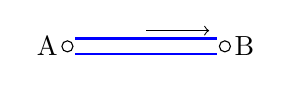
\begin{tikzpicture}
\draw (0,0) circle (2pt) node[left] {A};
\draw (2,0) circle (2pt) node[right] {B};
\draw[blue,thick] (0.1,0.1) -- (1.9,0.1);
\draw[blue,thick] (0.1,-0.1) -- (1.9,-0.1);
\draw[->] (1,0.2) -- (1.8,0.2);
\end{tikzpicture}
\caption{Pheromone trails and path selection}
\label{fig:aco_path}
\end{marginfigure}

\subsection{Differential Evolution (DE) Algorithm}
A vector-based evolutionary optimization algorithm. Provides effective results in continuous optimization problems.

\subsubsection{Basic Operators}
\begin{itemize}
    \item Mutation vector
    \item Crossover
    \item Selection
    \item Scaling factor (F)
    \item Crossover ratio (CR)
\end{itemize}

\begin{equation}
v_i = x_{r1} + F(x_{r2} - x_{r3})
\end{equation}

\begin{tcolorbox}[title=DE Strategies]
\begin{itemize}
    \item DE/rand/1/bin
    \item DE/best/1/bin
    \item DE/rand/2/bin
    \item DE/best/2/bin
    \item DE/current-to-best/1/bin
\end{itemize}
\end{tcolorbox}

\subsubsection{Algorithm Steps}
\begin{enumerate}
    \item Create initial population
    \item In each generation:
        \begin{itemize}
            \item Generate mutation vectors
            \item Apply crossover
            \item Perform selection
        \end{itemize}
    \item Continue until stopping criterion is met
\end{enumerate}

\sidenote{The differential evolution algorithm is particularly effective in continuous optimization problems. Parameter tuning is relatively easy and convergence speed is high.}

\subsection{Artificial Bee Colony (ABC) Optimization}
An optimization algorithm inspired by honey bees' food search behavior.

\subsubsection{Bee Types and Tasks}
\begin{itemize}
    \item Worker bees: Investigation of current resources
    \item Onlooker bees: Evaluation of promising resources
    \item Scout bees: Discovery of new resources
\end{itemize}

\begin{equation}
v_{ij} = x_{ij} + \phi_{ij}(x_{ij} - x_{kj})
\end{equation}

\begin{marginfigure}
\centering
\begin{tikzpicture}
\draw[->] (0,0) -- (4,0) node[right] {$x$};
\draw[->] (0,0) -- (0,4) node[above] {$f(x)$};
\filldraw[blue] (1,2) circle (2pt) node[above] {Worker};
\filldraw[red] (2,3) circle (2pt) node[above] {Onlooker};
\filldraw[green] (3,1) circle (2pt) node[above] {Scout};
\end{tikzpicture}
\caption{Role of different bee types in ABC}
\label{fig:abc_bees}
\end{marginfigure}

\subsubsection{Algorithm Steps}
\begin{enumerate}
    \item Determine initial food sources
    \item In each cycle:
        \begin{itemize}
            \item Worker bee phase
            \item Onlooker bee phase
            \item Scout bee phase
        \end{itemize}
    \item Continue until stopping criterion is met
\end{enumerate}

\subsection{Quantum and Hybrid Optimization Algorithms}
Approaches inspired by quantum mechanics principles and combining strengths of different algorithms.

\subsubsection{Quantum-Inspired Algorithms}
\begin{itemize}
    \item Quantum particle swarm
    \item Quantum genetic algorithm
    \item Quantum simulated annealing
\end{itemize}

\begin{equation}
\psi(x,t) = \frac{1}{\sqrt{2\pi\sigma^2}} e^{-\frac{(x-\mu)^2}{2\sigma^2}}
\end{equation}

\begin{tcolorbox}[title=Advantages of Quantum Mechanism]
\begin{itemize}
    \item Better exploration ability
    \item Avoiding local optima
    \item Fast convergence
    \item Utilizing uncertainty principle
\end{itemize}
\end{tcolorbox}

\subsection{Other Metaheuristic Optimization Algorithms}
Dozens of new metaheuristic optimization algorithms are added to the academic literature each year. Some of these algorithms can still present quite original approaches. However, within the basic classifications, many of them are developed by imitating certain mechanisms of previous algorithms to some extent. For an engineer looking at this topic from outside the academic perspective, understanding and being able to apply some basic algorithms is much more beneficial than constantly following new algorithms. Especially considering the development of artificial intelligence, what is really important is implementing theoretical knowledge in the right practical fields.   
\section{Ayrık Parametrelerin Optimizasyonu}
Ayrık (Discrete) değişkenler içeren optimizasyon problemlerinin çözüm yöntemleri bu bölümde incelenecektir. Özellikle yapısal sistemlerde karşılaşılan ayrık parametre optimizasyonu problemleri ve çözüm stratejileri ele alınacaktır.

\subsection{Ayrık ve Sürekli Optimizasyon Farkları}
Optimizasyon problemlerinin çözüm uzayı yapısına göre sınıflandırılması ve temel farklılıkların incelenmesi.

\subsubsection{Temel Farklılıklar}
\begin{itemize}
    \item Çözüm uzayının yapısı
    \item Kullanılabilecek yöntemler
    \item Hesaplama karmaşıklığı
    \item Gradyan bilgisinin kullanımı
\end{itemize}

\begin{tcolorbox}[title=Ayrık vs Sürekli Optimizasyon]
\begin{itemize}
    \item \textbf{Ayrık:}
        \begin{itemize}
            \item Kesikli çözüm uzayı
            \item Kombinatoryal yöntemler
            \item NP-zor problemler
            \item Gradyan kullanılamaz
        \end{itemize}
    \item \textbf{Sürekli:}
        \begin{itemize}
            \item Sürekli çözüm uzayı
            \item Gradyan tabanlı yöntemler
            \item Diferansiyellenebilirlik
            \item Lokal bilgi kullanımı
        \end{itemize}
\end{itemize}
\end{tcolorbox}

\subsection{Gezgin Satıcı Problemi (TSP)}
Ayrık optimizasyon problemlerinin klasik örneği olan TSP (Travelling Salesman Problem)\sidenote{
    
\qrcode[height=1in]{https://github.com/btayfur/structural-optimization/blob/main/Code/Examples/Exmp4}}, birçok gerçek dünya probleminin modellenmesinde kullanılır. Bu problem, bir satıcının belirli şehirleri en kısa mesafede dolaşması gerektiği senaryoyu ele alır. Her şehre yalnızca bir kez uğranması ve tur sonunda başlangıç noktasına dönülmesi gerekir. TSP, lojistik, üretim planlaması, PCB devre tasarımı ve DNA dizilimi gibi alanlarda uygulanır. Problemin çözüm uzayı, şehir sayısı arttıkça faktöriyel olarak büyüdüğünden (n şehir için n! olası tur), büyük ölçekli problemler için kesin çözüm bulmak hesaplama açısından oldukça zorludur.

\subsubsection{Problem Tanımı}
\begin{itemize}
    \item N şehir arasında en kısa turu bulma
    \item Her şehre bir kez uğrama
    \item Başlangıç noktasına dönme
    \item NP-zor problem sınıfı
\end{itemize}

\begin{equation}
\min \sum_{i=1}^n \sum_{j=1}^n d_{ij}x_{ij}
\end{equation}


\subsubsection{Çözüm Yaklaşımları}
\begin{itemize}
    \item Kesin yöntemler:
        \begin{itemize}
            \item Dal-sınır
            \item Tamsayılı programlama
        \end{itemize}
    \item Sezgisel yöntemler:
        \begin{itemize}
            \item En yakın komşu
            \item 2-opt, 3-opt
            \item Lin-Kernighan
        \end{itemize}
    \item Metasezgisel yöntemler:
        \begin{itemize}
            \item ACO
            \item GA
            \item Tabu arama
        \end{itemize}
\end{itemize}

\sidenote{TSP, ayrık optimizasyon problemlerinin prototip örneğidir. Birçok gerçek dünya problemi TSP'ye indirgenebilir. Ancak TSP için uygulanan her optimizasyon algoritması, bir başka problem için kullanılamayabilir. Dolayısıyla her optimizasyon problemi bazı yaygın problemlere benzese de, kendi özel yapısı gözönüne alınarak ele alınmalıdır.}

\subsection{Çelik Yapıların Kesit Optimizasyonu}
Ayrık optimizasyon problemlerinin, yapısal optimizasyonda en kolay karşılaşılacak örneği çelik yapıların kesit optimizasyonudur. Bu problemde, çelik yapılarda kullanılan standart kesitlerin seçimine dayalı bir optimizasyon problemi ele alınır.

\subsubsection{Problem Tanımı}
Çelik yapılarda kesit optimizasyonu, ayrık bir optimizasyon problemidir:
\begin{itemize}
    \item Standart kesit tabloları
    \item Yapısal kısıtlar
    \item Minimum ağırlık hedefi
    \item Gruplandırma gereksinimleri
\end{itemize}

\begin{equation}
\begin{aligned}
\min & \quad \sum_{i=1}^n \rho_i L_i A_i \\
\text{s.t.} & \quad \sigma_i \leq \sigma_{allow} \\
& \quad \delta \leq \delta_{allow} \\
& \quad A_i \in S
\end{aligned}
\end{equation}


\subsubsection{Çözüm Stratejileri}
\begin{itemize}
    \item Ayrık değişkenli optimizasyon
    \item Metasezgisel yöntemler
    \item Hibrit yaklaşımlar
    \item Paralel hesaplama
\end{itemize}

\begin{tcolorbox}[title=Optimizasyon Süreci]
\begin{enumerate}
    \item Yapısal analiz
    \item Kesit seçimi
    \item Kısıt kontrolü
    \item İteratif iyileştirme
\end{enumerate}
\end{tcolorbox}



\subsection{İndislerle Problem Çözümünün Basitleştirilmesi}
Çelik yapı optimizasyonu farklı biçimlerde ele alınabilir. Ancak eğer öntanımlı çelik kesitleri kullanıyorsa, kesit seçimi ayrık bir optimizasyon problemi olarak karşımıza çıkar. Bu durumda, kesit seçimi için bir veri yapısı oluşturmak ve bu veri yapısını kullanarak optimizasyon problemini çözmek gerekir. Bu noktada kesit listeleri indislenerek ele alınabilir. Ancak üzerine tartışılması gereken bir nokta şu olabilir: kesit listeleri hangi parametresi esas alınarak sıralanacak ve indislenecektir. Örneğin, yalnızca kesit alanının sıralamaya esas kabul edilmesi, eğilme mukavemeti açısından aynı sıralamanın oluşmasını garanti etmez. Fakat eğilme mukavemetinin esas alınması da aynı şekilde eksenel yük etkisi altında aynı sıralamanın oluşacağını garanti edemez. Dolayısıyla, problem özelinde kesit listelerinin farklı indisleme stratejisiyle ele alınması daha mantıklı olabilir. Örneğin, eksenel kuvvete maruz kalan elemanlarda kesit alanı esas alınırken, eğilme etkisin altındaki elemanlarda eğilme mukavemeti esas alınabilir. Veya daha etkili olacak farklı bir strateji geliştirebiliriz. 

\subsubsection{İndisleme Stratejisi}
\begin{itemize}
    \item Kesit grupları
    \item Eleman numaralandırma
    \item Düğüm noktaları
    \item Yükleme durumları
\end{itemize}

\begin{equation}
x_i = \text{ind}(A_i), \quad i = 1,\ldots,n
\end{equation}

\sidenote{İndisleme, ayrık optimizasyon problemlerinin çözümünü kolaylaştırır ve hesaplama verimliliğini artırır.}

\subsubsection{Veri Yapıları}
\begin{itemize}
    \item Kesit özellikleri tablosu
    \item Bağlantı matrisi
    \item Kısıt matrisi
    \item İndis dönüşüm tablosu
\end{itemize}

\begin{tcolorbox}[title=Veri Yapısı Örneği]
\begin{verbatim}
sections = {
    1: {'A': 10.3, 'I': 171},
    2: {'A': 13.2, 'I': 375},
    ...
}
\end{verbatim}
\end{tcolorbox}

\subsection{Optimizasyon Sonuçlarının Değerlendirilmesi}
Ayrık optimizasyon problemlerinin çözüm kalitesinin ve performansının analizi.

\subsubsection{Performans Ölçütleri}
\begin{itemize}
    \item Toplam ağırlık
    \item Maksimum gerilme oranı
    \item Maksimum deplasman
    \item Hesaplama süresi
\end{itemize}

\subsubsection{Sonuçların Görselleştirilmesi}
\begin{itemize}
    \item Yakınsama grafikleri
    \item Gerilme dağılımları
    \item Deplasman şekilleri
    \item Kesit dağılımları
\end{itemize}
  
\section{Optimization of Continuous Parameters}
Optimization of continuous parameters is commonly encountered in structural engineering and other engineering fields. In this section, the fundamental characteristics, mathematical formulation, and solution methods of optimization problems expressed with continuous variables will be examined.

\subsection{Basic Concepts of Continuous Optimization}
Continuous optimization refers to optimization problems where design variables can take continuous values. In such problems, the design space consists of an infinite number of points, and variables can take any real value.

\subsubsection{Continuous Design Variables}
Continuous design variables are parameters that can take any value within a specific range. For example:
\begin{itemize}
    \item Cross-sectional dimensions of a beam (width, height)
    \item Material properties (elasticity modulus, density)
    \item Geometric parameters (angles, lengths)
    \item Control parameters (force magnitudes, damping coefficients)
\end{itemize}

\subsubsection{General Form of Continuous Optimization Problems}
Continuous optimization problems are generally expressed in the following form:
\begin{align}
\min_{\mathbf{x}} \quad & f(\mathbf{x}) \\
\text{s.t.} \quad & g_i(\mathbf{x}) \leq 0, \quad i = 1, 2, \ldots, m \\
& h_j(\mathbf{x}) = 0, \quad j = 1, 2, \ldots, p \\
& \mathbf{x}_L \leq \mathbf{x} \leq \mathbf{x}_U
\end{align}

Where:
\begin{itemize}
    \item $\mathbf{x} \in \mathbb{R}^n$ : Vector of design variables
    \item $f(\mathbf{x})$ : Objective function
    \item $g_i(\mathbf{x})$ : Inequality constraints
    \item $h_j(\mathbf{x})$ : Equality constraints
    \item $\mathbf{x}_L, \mathbf{x}_U$ : Lower and upper bounds
\end{itemize}

\begin{tcolorbox}[title=Continuous Optimization Example]
Weight minimization problem of a cantilever beam:
\begin{align}
\min_{b,h} \quad & \rho \cdot L \cdot b \cdot h \\
\text{s.t.} \quad & \sigma_{max} = \frac{6PL}{bh^2} \leq \sigma_{allow} \\
& \delta_{max} = \frac{PL^3}{3EI} \leq \delta_{allow} \\
& b_{min} \leq b \leq b_{max} \\
& h_{min} \leq h \leq h_{max}
\end{align}

Where $b$ and $h$ are the width and height of the beam, respectively.
\end{tcolorbox}

\sidenote{In continuous optimization problems, the objective function and constraints are generally continuous and differentiable functions, which allows the use of gradient-based optimization methods.}

\subsection{Mathematical Formulation of Continuous Optimization Problems}

The mathematical formulation of continuous optimization problems is a fundamental step that determines the nature of the problem and solution methods. This formulation includes the mathematical expression of the objective function, constraints, and design variables.

\subsubsection{Objective Function}
The objective function mathematically expresses the engineering performance criterion to be optimized. Commonly used objective functions in structural optimization problems are:

\begin{itemize}
    \item \textbf{Weight minimization:} $f(\mathbf{x}) = \sum_{i=1}^{n} \rho_i V_i(\mathbf{x})$
    \item \textbf{Flexibility minimization:} $f(\mathbf{x}) = \mathbf{F}^T \mathbf{u}(\mathbf{x})$
    \item \textbf{Stress minimization:} $f(\mathbf{x}) = \max_{i} \sigma_i(\mathbf{x})$
    \item \textbf{Displacement minimization:} $f(\mathbf{x}) = \max_{i} |u_i(\mathbf{x})|$
    \item \textbf{Frequency maximization:} $f(\mathbf{x}) = -\omega_1(\mathbf{x})$ (first natural frequency)
    \item \textbf{Cost minimization:} $f(\mathbf{x}) = \sum_{i=1}^{n} c_i x_i$
\end{itemize}

\subsubsection{Constraint Functions}
Constraint functions are mathematical expressions that ensure the design meets certain requirements. Constraints frequently used in structural optimization problems are:

\begin{itemize}
    \item \textbf{Stress constraints:} $g_i(\mathbf{x}) = \sigma_i(\mathbf{x}) - \sigma_{allow} \leq 0$
    \item \textbf{Displacement constraints:} $g_i(\mathbf{x}) = |u_i(\mathbf{x})| - u_{allow} \leq 0$
    \item \textbf{Buckling constraints:} $g_i(\mathbf{x}) = P_{cr,i}(\mathbf{x}) - P_{applied} \leq 0$
    \item \textbf{Frequency constraints:} $g_i(\mathbf{x}) = \omega_{min} - \omega_i(\mathbf{x}) \leq 0$
    \item \textbf{Equilibrium constraints:} Express that the structure must satisfy static equilibrium conditions.
    \item \textbf{Geometric constraints:} Express that design variables must satisfy certain geometric relationships.
\end{itemize}

\subsubsection{Sensitivity Analysis}
Sensitivity analysis involves calculating the derivatives of the objective function and constraints with respect to design variables. These derivatives are used to determine the search direction in gradient-based optimization algorithms.

\begin{equation}
\nabla f(\mathbf{x}) = \left[ \frac{\partial f}{\partial x_1}, \frac{\partial f}{\partial x_2}, \ldots, \frac{\partial f}{\partial x_n} \right]^T
\end{equation}

\begin{equation}
\nabla g_i(\mathbf{x}) = \left[ \frac{\partial g_i}{\partial x_1}, \frac{\partial g_i}{\partial x_2}, \ldots, \frac{\partial g_i}{\partial x_n} \right]^T
\end{equation}

Methods used for sensitivity analysis:
\begin{itemize}
    \item \textbf{Analytical methods:} Direct calculation of derivatives using mathematical expressions
    \item \textbf{Finite difference method:} Numerical approximation of derivatives
    \item \textbf{Adjoint method:} Used for efficient sensitivity calculation in complex systems
    \item \textbf{Automatic differentiation:} Automatic derivative calculation by computer programs
\end{itemize}

\subsubsection{Distinctive Characteristics of Continuous Optimization}
Continuous optimization problems, unlike discrete optimization problems, are those where design variables can take continuous values. The distinctive characteristics of these problems are:

\begin{itemize}
    \item \textbf{Continuous design space:} Design variables can take values from the set of real numbers, meaning an infinite number of possible solutions.
    
    \item \textbf{Differentiability:} The objective function and constraints are generally differentiable functions, allowing the use of gradient-based optimization methods.
    
    \item \textbf{Convexity:} Whether the problem formulation is convex determines the achievability of the global optimum. In convex problems, the local optimum is also the global optimum.
    
    \item \textbf{Continuity:} The continuity of functions ensures more stable operation of the optimization algorithm.
    
    \item \textbf{Differentiability:} The existence of higher-order derivatives allows the use of Newton-like methods.
\end{itemize}

Continuous optimization problems are commonly used in structural engineering for optimizing variables such as cross-sectional dimensions, material properties, or geometric parameters. In solving these problems, gradient-based methods (Newton's method, conjugate gradient method), gradient-free methods (Nelder-Mead simplex method), or metaheuristic algorithms (genetic algorithm, particle swarm optimization) can be used.

\subsection{General Applications of Continuous Optimization in Structural Optimization}
Although two common optimization problems have been exemplified at this point, many outputs calculated depending on parameters can be considered and improved as optimization problems.

\subsubsection{Non-Predefined Size Optimization}
Non-predefined size optimization involves considering cross-sectional dimensions of structural elements as continuous variables without being limited by standard catalog values. This approach provides designers with a wider design space and enables the potential to obtain more efficient structures. In traditional approaches, while selection is made from certain standard sections (e.g., I-profiles, box sections) for structural elements, in non-predefined optimization, section properties (area, moment of inertia, etc.) are used directly as design variables.

In such optimization problems, objectives such as minimum weight or maximum stiffness are generally pursued while considering structural constraints such as stress, displacement, and buckling. The section properties obtained as a result of optimization are then interpreted to be converted into manufacturable sections or produced as special sections. Non-predefined size optimization is commonly used in aerospace, space, and automotive industries to minimize material usage while maximizing performance.

\subsubsection{Topological Optimization}
Topological optimization is an advanced structural optimization method used to determine the most efficient material distribution of a structure. This method optimizes the basic form and connection structure of the structure by deciding where material should and should not be located within a specific design area. Unlike traditional optimization methods, it can change not only the dimensions or shape but also the topology of the structure.

The topological optimization process generally begins with dividing a design area into finite elements and assigning a design variable representing material density to each element. The optimization algorithm adjusts these variables to find the best material distribution under certain constraints (e.g., maximum weight or minimum flexibility). As a result, highly efficient and lightweight structures, often resembling those found in nature, emerge. This method is widely used in various fields such as designing lightweight parts in automotive and aerospace industries, developing medical implants, and creating optimized structures for 3D printing technologies.   
\section{Introduction to Structural Optimization}
Although structural optimization has been treated as a different type of optimization, it essentially progresses with similar principles to all optimization problems. However, the definition of the problem, and consequently the selection of effective solution algorithms, depends on engineering judgment. In this section, we will try to explain how the concepts defined under classical optimization topics transform into a context in structural optimization.

\subsection{Structural Optimization Terminology}

\subsubsection{Objective Functions}
In structural optimization, the objective function mathematically expresses the engineering target to be optimized. The most commonly used objective functions in structural design are:\sidenote{In multi-objective optimization problems, multiple objective functions can be weighted and converted into a single function, or Pareto-optimal solutions can be sought.}

\begin{itemize}
    \item \textbf{Weight minimization:} Aims to minimize the total weight of the structure. Particularly critical in aerospace structures.
    \item \textbf{Cost minimization:} Aims to minimize the production, material, and labor costs of the structure.
    \item \textbf{Stiffness maximization:} Aims to maximize the structure's resistance to deformation under specific loads.
    \item \textbf{Strength maximization:} Aims to increase the maximum load the structure can carry.
    \item \textbf{Energy dissipation:} Optimizes the structure's energy dissipation capacity under dynamic loads.
\end{itemize}

\subsubsection{Constraints}
In structural optimization, constraints define the conditions that must be met for the design to be feasible. These constraints are the structural engineering counterparts of mathematical constraints in classical optimization problems:

\begin{itemize}
    \item \textbf{Stress constraints:} Ensures that stresses in the structure do not exceed allowed maximum values. For example: $\sigma_i \leq \sigma_{allow}$
    
    \item \textbf{Displacement constraints:} Ensures that displacements in the structure remain within certain limits. For example: $\delta_i \leq \delta_{allow}$
    
    \item \textbf{Buckling constraints:} Ensures that the buckling loads of structural elements are greater than the applied loads by a certain safety factor.
    
    \item \textbf{Vibration constraints:} Ensures that the natural frequencies of the structure are above or below certain values.
    
    \item \textbf{Geometric constraints:} In the context of structural optimization, ensures that design variables remain within physically feasible limits. For example:
    \begin{itemize}
        \item Minimum and maximum cross-sectional dimensions
        \item Minimum wall thicknesses
        \item Connection requirements between elements\sidenote{For example, it may be desired that the cross-sectional dimensions used in the upper floors of a steel structure be larger than those in the lower floors, which is also quite logical from an application perspective.}
        \item Assembly and manufacturing constraints
    \end{itemize}
    
    \item \textbf{Equilibrium constraints:} Expresses that the structure must satisfy static equilibrium conditions.
    
    \item \textbf{Compatibility constraints:} Specifies that deformations must be continuous and compatible.
\end{itemize}

\begin{tcolorbox}[title=Example of Structural Optimization Constraints]
In a bridge design:
\begin{align}
\sigma_{max} &\leq 250 \text{ MPa} \quad \text{(Stress constraint)} \\
\delta_{mid} &\leq L/400 \quad \text{(Displacement constraint)} \\
f_1 &\geq 2.0 \text{ Hz} \quad \text{(Vibration constraint)} \\
t_{min} &\geq 8 \text{ mm} \quad \text{(Geometric constraint)}
\end{align}
\end{tcolorbox}

\sidenote{The mathematical formulation of constraints is expressed based on the results of finite element analysis and is generally in the form of nonlinear functions.}

\subsubsection{Design Variables}
In structural optimization, design variables represent the parameters to be optimized. These variables are parameters that can be changed by the optimization algorithm and adjusted to find the best solution. Common design variables used in structural engineering are:

\begin{itemize}
    \item \textbf{Cross-sectional properties:} 
    \begin{itemize}
        \item Profile dimensions (width, height)
        \item Wall thicknesses
        \item Cross-sectional area
        \item Moment of inertia
    \end{itemize}
    
    \item \textbf{Material properties:} 
    \begin{itemize}
        \item Elasticity modulus
        \item Density
        \item Yield strength
    \end{itemize}
    
    \item \textbf{Geometric parameters:} 
    \begin{itemize}
        \item Node point coordinates
        \item Curvature radii
        \item Angles
    \end{itemize}
    
    \item \textbf{Topological parameters:} 
    \begin{itemize}
        \item Material presence/absence (0-1 variables)
        \item Material density (continuous variables varying between 0-1)\sidenote{In many computational methods requiring optimization or regression-like coding, a normalization approach is used to handle data in a more standard way. This approach ensures that data has a value range varying between 0-1. The smallest data in the existing data becomes 0, and the largest data becomes 1. All intermediate values take a proportional value within this range.}
        \item Presence of connection points
    \end{itemize}
\end{itemize}

\begin{tcolorbox}[title=Design Variables Representation]
In a typical steel frame optimization, design variables can be represented as:
\begin{align}
\mathbf{x} = [A_1, A_2, \ldots, A_n, I_{y1}, I_{y2}, \ldots, I_{yn}, I_{z1}, I_{z2}, \ldots, I_{zn}]^T
\end{align}
Where $A_i$ represents cross-sectional areas, and $I_{yi}$ and $I_{zi}$ represent moments of inertia.
\end{tcolorbox}

\subsection{Structural Optimization Categories}

Structural optimization problems can be categorically divided into some basic headings (Shape, size, topology, etc.). However, an engineer can consider any problem with parameters producing conflicting outputs as an optimization problem.

For example, making a structure lighter often means compromising stress capacities. These conflicting outputs are the result of the same parameters.

\subsubsection{Size Optimization}
Size optimization is the optimization of cross-sectional dimensions of elements while keeping the general geometry of the structure constant. It is the most basic and commonly used structural optimization approach.

\begin{itemize}
    \item \textbf{Design variables:} Cross-sectional properties such as area, thickness, width-height
    \item \textbf{Advantages:} 
    \begin{itemize}
        \item Relatively simpler mathematical formulation
        \item Suitable for improving existing designs
        \item Widespread use in industry
    \end{itemize}
    \item \textbf{Application areas:} Steel structures, frame systems, truss systems
\end{itemize}

\subsubsection{Shape Optimization}
Shape optimization is performed by changing the shapes of structural elements or positions of node points. The general topology of the structure is preserved while the boundary geometry is changed.

\begin{itemize}
    \item \textbf{Design variables:} Node point coordinates, curvature parameters, control points
    \item \textbf{Advantages:} 
    \begin{itemize}
        \item More design flexibility compared to size optimization
        \item Effective in reducing stress concentrations
    \end{itemize}
    \item \textbf{Challenges:} 
    \begin{itemize}
        \item Geometric changes may require remeshing of the finite element mesh
        \item Complex mathematical formulation
    \end{itemize}
    \item \textbf{Application areas:} Aerospace structures, automotive parts, bridge constructions
\end{itemize}

\subsubsection{Topology Optimization}
Topology optimization is performed by changing the basic structure or topology of the structure. The distribution of material within the structure is optimized, and regions where material should or should not be present are generally determined.

\begin{itemize}
    \item \textbf{Design variables:} Material density, material presence/absence
    \item \textbf{Advantages:} 
    \begin{itemize}
        \item Highest design freedom
        \item Ability to produce innovative and unpredictable designs
        \item Significant potential for material savings
    \end{itemize}
    \item \textbf{Challenges:} 
    \begin{itemize}
        \item Mathematically and computationally complex
        \item Difficult to apply manufacturability constraints
        \item Interpretation of results and conversion to feasible designs
    \end{itemize}
    \item \textbf{Application areas:} Aerospace, automotive, medical implants, 3D printed structures
\end{itemize}

\begin{tcolorbox}[title=Example: Cantilever Beam Optimization]
Optimization of the same cantilever beam problem with three different approaches:

\textbf{Size:} The variation of beam cross-section height along the length is optimized.

\textbf{Shape:} The shape of the beam's upper and lower surfaces is optimized.

\textbf{Topology:} The material distribution in the beam's internal structure is optimized, usually resulting in a truss-like structure.
\end{tcolorbox}

\subsection{Structural Optimization Formulation}

A structural optimization problem can be mathematically expressed as:

\begin{align}
\text{Minimize: } & f(\mathbf{x}) \\
\text{Constraints: } & g_j(\mathbf{x}) \leq 0, \quad j = 1, 2, \ldots, m \\
& h_k(\mathbf{x}) = 0, \quad k = 1, 2, \ldots, p \\
& \mathbf{x}_L \leq \mathbf{x} \leq \mathbf{x}_U
\end{align}

Where:
\begin{itemize}
    \item $\mathbf{x}$ : vector of design variables
    \item $f(\mathbf{x})$ : objective function (for minimization problem)
    \item $g_j(\mathbf{x})$ : inequality constraints
    \item $h_k(\mathbf{x})$ : equality constraints
    \item $\mathbf{x}_L$ and $\mathbf{x}_U$ : lower and upper bounds of design variables
\end{itemize}

\subsubsection{Connection with Finite Element Analysis}
In structural optimization problems, the objective function and constraints are generally dependent on finite element analysis (FEA) results. This connection can be expressed as:

\begin{align}
\mathbf{K}(\mathbf{x}) \mathbf{u} &= \mathbf{F} \\
f(\mathbf{x}) &= f(\mathbf{x}, \mathbf{u}(\mathbf{x})) \\
g_j(\mathbf{x}) &= g_j(\mathbf{x}, \mathbf{u}(\mathbf{x})) \\
h_k(\mathbf{x}) &= h_k(\mathbf{x}, \mathbf{u}(\mathbf{x}))
\end{align}

Where:
\begin{itemize}
    \item $\mathbf{K}(\mathbf{x})$ : stiffness matrix dependent on design variables
    \item $\mathbf{u}$ : displacement vector
    \item $\mathbf{F}$ : external force vector
\end{itemize}

\begin{tcolorbox}[title=Structural Optimization Algorithm Selection]
Algorithm selection in structural optimization problems depends on the following factors:
\begin{itemize}
    \item Problem size (number of design variables)
    \item Number and complexity of constraints
    \item Computational cost of function evaluations
    \item Characteristic of design space (existence of multiple local optima)
    \item Availability of sensitivity information
\end{itemize}
\end{tcolorbox}   
\section{Topological Optimization}
This section will examine topological optimization methods that aim to determine the most basic form of structural systems. The optimization of material distribution and modern topology optimization techniques will be discussed.

\subsection{Foundations of Topological Optimization}
Topological optimization is an advanced structural optimization method used to determine the most efficient material distribution of a structure. Unlike traditional optimization methods, topological optimization optimizes not only the dimensions or shape but also the basic form and connection structure of the structure. In this approach, decisions are made about where material should and should not be located within a specific design area.

The topological optimization process generally begins with dividing a design area into finite elements. Each element is assigned a design variable representing material density, varying between 0 and 1. The optimization algorithm adjusts these variables to find the best material distribution under certain constraints (e.g., maximum weight or minimum flexibility). As a result, highly efficient and lightweight structures, often resembling those found in nature, emerge.

This method is widely used in various fields such as designing lightweight and durable parts in automotive and aerospace industries, developing medical implants, and creating optimized structures for 3D printing technologies. Topological optimization provides engineers with the opportunity to offer innovative and efficient solutions that would be difficult to achieve with traditional design approaches.

\subsubsection{Basic Concepts}
\begin{itemize}
    \item Material distribution \sidenote{Distribution showing how material is placed within the design area, generally expressed with density variables.}
    \item Structural topology \sidenote{Geometric arrangement defining the basic form, connection structure, and material distribution of a structure.}
    \item Homogenization \sidenote{Method for calculating effective properties of composite materials, used to determine macro properties of microstructures.}
    \item Design variables \sidenote{Parameters that can be changed during the optimization process, generally assigned to each finite element and representing material presence.}
\end{itemize}

\begin{equation}
\min_{x \in [0,1]^n} \quad c(x) = F^T U(x)
\end{equation}

\subsection{Relationship Between Finite Element Method and Optimization}
Topological optimization is directly related to the Finite Element Method (FEM) and this method is a fundamental component of the optimization process. The finite element method allows analyzing complex geometries by dividing them into smaller and simpler elements, enabling precise calculation of structural behavior necessary for topological optimization.

In the optimization process, when the material distribution changes in each iteration, the mechanical behavior of the structure (stresses, displacements, natural frequencies, etc.) is recalculated using finite element analysis. These analysis results enable the optimization algorithm to decide where to add or remove material in the next step. Thus, FEM becomes an integral part of both the analysis and decision-making mechanism of topological optimization.

\subsubsection{FEM Formulation}
\begin{itemize}
    \item Stiffness matrix
    \item Load vector
    \item Displacement field
    \item Element types
\end{itemize}

\begin{equation}
K(x)U = F
\end{equation}

\subsubsection{Creation of Finite Element Model with API}
Various software offer Application Programming Interface (API) for creating and analyzing finite element models. These APIs enable topological optimization algorithms to work integrated with finite element analyses. Especially in optimization processes requiring automatic iteration, API usage provides great efficiency by eliminating manual model creation and analysis processes.

SAP2000 OAPI (Open Application Programming Interface) is a commonly used API example for structural analysis and optimization. This interface provides access to all features of SAP2000 software through programming languages such as Python, MATLAB, or C++. In the topological optimization process, the algorithm can use SAP2000 OAPI in each iteration to:

\begin{itemize}
    \item Apply updated material properties to the model
    \item Run the analysis automatically
    \item Read analysis results (stresses, displacements, etc.)
    \item Calculate new material distribution based on these results
\end{itemize}

Such API integrations enable complete automation of the topological optimization process, allowing even complex structures to be optimized efficiently. Additionally, other finite element software such as ANSYS, Abaqus, and NASTRAN also offer similar APIs. More detailed examples using SAP2000 OAPI will be examined in later topics.

\subsection{Density-Based Methods}
The most commonly used density-based topological optimization method is SIMP (Solid Isotropic Material with Penalization). This method works by assigning a density variable varying between 0 and 1 to each finite element. Here, 0 represents material absence and 1 represents full material presence.

The basic principle of the SIMP method is to penalize intermediate density values (values between 0 and 1) to obtain a more distinct 0-1 distribution as a result of optimization. This is achieved by defining material properties (e.g., elasticity modulus) as a power function of the density variable. The penalty parameter is generally chosen as 3 or higher.

The SIMP method has been successfully used in various engineering applications such as lightweighting automotive parts, optimizing aircraft structural elements, and designing medical implants. The method has become a standard approach in industry due to its well-defined mathematical foundation and compatibility with gradient-based optimization algorithms.

\subsubsection{SIMP Method}
Solid Isotropic Material with Penalization:
\begin{equation}
E(x) = E_{min} + x^p(E_0 - E_{min})
\end{equation}

\begin{itemize}
    \item Density variables: $x \in [0,1]$
    \item Penalty parameter: $p > 1$
    \item Minimum stiffness: $E_{min}$
    \item Full material stiffness: $E_0$
\end{itemize}

\begin{tcolorbox}[title=Advantages of SIMP Method]
\begin{itemize}
    \item Simple implementation
    \item Fast convergence
    \item Penalization of intermediate densities
    \item Widespread use in industrial applications
\end{itemize}
\end{tcolorbox}

\subsection{ESO and BESO Methods}
Evolutionary Structural Optimization (ESO) and Bi-directional Evolutionary Structural Optimization (BESO) methods are heuristic approaches used in structural topology optimization. The ESO method is based on the principle of "gradually removing inefficient material" and aims to reach the optimum design by removing elements with low stress or energy density from the structure. BESO is an improved version of ESO and includes not only material removal but also material addition to necessary regions. Although these methods do not have as solid a mathematical foundation as SIMP, they are preferred in engineering applications due to their ease of implementation and intuitive understanding.

\subsection{Level-Set Method}
The Level-Set method is a mathematical approach used to explicitly define structure boundaries in topology optimization. In this method, the boundaries of the structure are represented as the zero-level curve (or surface) of a level-set function. During the optimization process, this level-set function is updated using Hamilton-Jacobi equations, thus allowing the structure boundaries to evolve smoothly. The Level-Set method has advantages such as creating sharp and clear boundaries, naturally handling topology changes, and easily incorporating manufacturability constraints. It is particularly effective in fluid-structure interaction problems and multi-material designs.   
\section{Boyut ve Şekil Optimizasyonu}
Yapısal sistemlerin boyut ve şekil parametrelerinin optimizasyonu, daha genel bir ifadeyle kesit optimizasyonu olarak da adlandırılabilir. Probleme bağlı olarak bunlardan biri veya ikisi aynı anda problemin parametresi haline gelebilir.

\subsection{Boyut Optimizasyonunun Temelleri}
Boyut optimizasyonu, yapısal sistemlerin kesit özelliklerinin (genişlik, yükseklik, kalınlık, vb.) en uygun değerlerini belirlemek için kullanılan bir optimizasyon yöntemidir. Bu yöntem, yapının topolojisini değiştirmeden, sadece elemanların boyutlarını değiştirerek optimum tasarıma ulaşmayı hedefler.

\subsubsection{Problem Parametreleri}
Boyut optimizasyonunda kullanılan tasarım değişkenleri genellikle şunları içerir:
\begin{itemize}
    \item \textbf{Kesit boyutları:} Kirişlerin genişlik ve yükseklikleri, plakaların kalınlıkları
    \item \textbf{Kesit alanları:} Çubuk elemanların kesit alanları
    \item \textbf{Atalet momentleri:} Kirişlerin eğilme ve burulma rijitliklerini belirleyen parametreler
    \item \textbf{Malzeme özellikleri:} Elastisite modülü, yoğunluk gibi değişkenler
    \item \textbf{Takviye elemanları:} Güçlendirme elemanlarının boyutları ve konumları
\end{itemize}

\subsubsection{Problem Çıktıları}
Boyut optimizasyonu sonucunda elde edilen çıktılar şunlardır:
\begin{itemize}
    \item \textbf{Optimum kesit boyutları:} Her yapı elemanı için en uygun boyutlar
    \item \textbf{Minimum ağırlık/maliyet:} Optimizasyon sonucunda elde edilen yapının toplam ağırlığı veya maliyeti
    \item \textbf{Yapısal performans göstergeleri:} Gerilmeler, deplasmanlar, doğal frekanslar
    \item \textbf{Malzeme kullanım verimliliği:} Her elemanın taşıma kapasitesinin ne kadar verimli kullanıldığı
    \item \textbf{Duyarlılık bilgileri:} Tasarım değişkenlerindeki değişimlerin amaç fonksiyonu üzerindeki etkileri
\end{itemize}

\subsubsection{Kısıtlayıcılar ve Karar Mekanizması}
Boyut optimizasyonunda, çeşitli kısıtlayıcılar problemin çözüm uzayını sınırlandırır ve karar mekanizmasını etkiler:

\begin{itemize}
    \item \textbf{Gerilme kısıtları:} $\sigma_{max} \leq \sigma_{allow}$
    \begin{itemize}
        \item Yapıdaki maksimum gerilmelerin izin verilen değerleri aşmaması gerekir
        \item Elemanların boyutlarını artırma yönünde etki yapar
    \end{itemize}
    
    \item \textbf{Deplasman kısıtları:} $\delta_{max} \leq \delta_{allow}$
    \begin{itemize}
        \item Yapıdaki maksimum yer değiştirmelerin belirli sınırlar içinde kalmasını sağlar
        \item Genellikle yapının rijitliğini artırma yönünde etki eder
    \end{itemize}
    
    \item \textbf{Burkulma kısıtları:} $P_{cr} \geq P_{design}$
    \begin{itemize}
        \item Basınç elemanlarının burkulma yüklerinin tasarım yükünden büyük olmasını sağlar
        \item Narin elemanların boyutlarını artırma yönünde etki yapar
    \end{itemize}
    
    \item \textbf{Frekans kısıtları:} $\omega_i \geq \omega_{min}$ veya $\omega_i \leq \omega_{max}$
    \begin{itemize}
        \item Yapının doğal frekanslarının belirli aralıklarda olmasını sağlar
        \item Dinamik yüklere maruz yapılarda önemlidir
    \end{itemize}
    
    \item \textbf{Üretilebilirlik kısıtları:} $x_{min} \leq x \leq x_{max}$
    \begin{itemize}
        \item Tasarım değişkenlerinin pratik üretim sınırları içinde kalmasını sağlar
        \item Çözüm uzayını gerçekçi değerlerle sınırlar
    \end{itemize}
    
    \item \textbf{Geometrik kısıtlar:} Örneğin $h/b \leq \alpha$
    \begin{itemize}
        \item Kesit oranlarının belirli sınırlar içinde kalmasını sağlar
        \item Yerel burkulma ve stabilite sorunlarını önler
    \end{itemize}
\end{itemize}

\begin{tcolorbox}[title=Boyut Optimizasyonu Süreci]
\begin{enumerate}
    \item Başlangıç tasarımının oluşturulması
    \item Yapısal analiz (FEM) ile performans değerlendirmesi
    \item Duyarlılık analizi ile tasarım değişkenlerinin etkilerinin belirlenmesi
    \item Optimizasyon algoritması ile tasarım değişkenlerinin güncellenmesi
    \item Yakınsama sağlanana kadar 2-4 adımlarının tekrarlanması
\end{enumerate}
\end{tcolorbox}

Boyut optimizasyonu, yapısal mühendislikte çelik yapıların kesit optimizasyonu, betonarme yapıların donatı optimizasyonu, köprü ve kule tasarımı gibi birçok uygulamada yaygın olarak kullanılmaktadır. Optimizasyon sonucunda, malzeme kullanımı azaltılırken yapısal performans gereksinimleri karşılanmakta, böylece daha ekonomik ve sürdürülebilir tasarımlar elde edilmektedir.


\subsection{Şekil Optimizasyonunun Temelleri}
Yapı elemanlarının dış sınırlarının ve iç boşluklarının optimizasyonu veya mühendisin konuyu bakış biçimine bağlı olarak farklı şekillerde ele alınabilir.

\begin{itemize}
    \item \textbf{Sınır Temsili:} Geometrik parametreler
    \item \textbf{Kontrol Noktaları:} Şekil değişimi kontrolü
    \item \textbf{Düzgünlük:} Geometrik süreklilik
\end{itemize}

\sidenote{Şekil optimizasyonu, topolojiyi değiştirmeden yapının geometrisini iyileştirir.}

\subsection{Matematiksel Formülasyon}
Boyut ve şekil optimizasyonu problemlerinin matematiksel ifadesi:

\begin{equation}
\begin{aligned}
& \text{minimize} & & f(\mathbf{x}, \mathbf{s}) \\
& \text{subject to} & & g_i(\mathbf{x}, \mathbf{s}) \leq 0, & & i = 1,\ldots,m \\
& & & h_j(\mathbf{x}, \mathbf{s}) = 0, & & j = 1,\ldots,p \\
& & & \mathbf{x}^L \leq \mathbf{x} \leq \mathbf{x}^U \\
& & & \mathbf{s}^L \leq \mathbf{s} \leq \mathbf{s}^U
\end{aligned}
\end{equation}

Burada:
\begin{itemize}
    \item \(\mathbf{x}\): Boyut parametreleri
    \item \(\mathbf{s}\): Şekil parametreleri
    \item \(f\): Amaç fonksiyonu
    \item \(g_i, h_j\): Kısıt fonksiyonları
\end{itemize}

\subsection{Parametrik Modelleme}
Tasarım değişkenlerinin matematiksel temsili:

\begin{itemize}
    \item \textbf{CAD Parametreleri:} Geometrik boyutlar
    \item \textbf{Spline Eğrileri:} Sınır temsili
    \item \textbf{Morph Box:} Şekil deformasyonu
\end{itemize}


\subsection{Duyarlılık Analizi}
Bazı yapısal optimizasyon problemlerinde tasarım değişkenleri (parametreler) için duyarlılık analizi yapılabilir. Fakat yapısal optimizasyon problemleri genellikle hiperstatik yapıda olduğundan, duyarlılık analizleri beklenen sonuçları veremez ve hatta yanıltıcı olabilir. \sidenote{Hiperstatiklik konusu, optimizasyon açısından önemlidir. Örneğin bir parametre için seçilen kesit, limit dayanıma yakın olmasına rağmen, yapının bir başka parametresindeki kesitin değişimi yük dağılımını tamamen etkileyerek, ilk kesitin gerrilmesini sınır dayanımın çok daha altına düşürebilir veya üzerine çıkarabilir.}


\subsection{Kısıt İşleme}
Tasarım kısıtlarının ele alınması:

\begin{itemize}
    \item \textbf{Gerilme Kısıtları:} Malzeme dayanımı
    \item \textbf{Deplasman Kısıtları:} Şekil değiştirme limitleri
    \item \textbf{Geometrik Kısıtlar:} Üretilebilirlik
\end{itemize}

\subsection{Çok Amaçlı Optimizasyon}
Daha sonra çok amaçlı optimizasyon konusundan çok daha ayrıntılı bir şekilde bahsedilecektir.

\begin{tcolorbox}[title=Çok Amaçlı Yaklaşımlar]
\begin{itemize}
    \item \textbf{Pareto Optimizasyonu:} Trade-off analizi
    \item \textbf{Ağırlıklı Toplam:} Tek amaç fonksiyonu
    \item \textbf{Hedef Programlama:} İdeal nokta yaklaşımı
\end{itemize}
\end{tcolorbox}

\subsection{Mesh Adaptasyonu}
Sonlu eleman modellerinde sıklıkla kabusa dönüşebilen mesh oluşturma süreci de zaman zaman optimizasyonun konusu olabilmektedir. Fakat bu konu ayrı bir uzmanlık alanının ve dersin konusudur.

\begin{itemize}
    \item \textbf{Mesh Kalitesi:} Eleman şekli kontrolü
    \item \textbf{Adaptif Mesh:} Otomatik ağ iyileştirme
    \item \textbf{Remeshing:} Yeniden ağ oluşturma
\end{itemize}

\subsection{Üretilebilirlik ve Pratik Kısıtlar}
Tasarımın pratik uygulanabilirliği:

\begin{itemize}
    \item \textbf{Standart Kesitler:} Katalog seçimi
    \item \textbf{İmalat Yöntemi:} Üretim kısıtları
    \item \textbf{Maliyet:} Ekonomik faktörler
\end{itemize}

\sidenote{Üretilebilirlik kısıtları, teorik optimum ile pratik çözüm arasında denge kurmayı gerektirir ve bu da bambaşka bir optimizasyon problemi olarak ele alınabilir.}

\subsection{Optimizasyon Sonuçlarının Değerlendirilmesi}
Elde edilen sonuçların analizi ve yorumlanması:

\begin{tcolorbox}[title=Değerlendirme Kriterleri]
\begin{itemize}
    \item \textbf{Performans İyileştirmesi:} Başlangıç durumuna göre kazanımlar
    \item \textbf{Kısıt Sağlama:} Tüm tasarım kısıtlarının kontrolü
    \item \textbf{Üretilebilirlik:} Pratik uygulanabilirlik analizi
    \item \textbf{Maliyet Analizi:} Ekonomik değerlendirme
\end{itemize}
\end{tcolorbox}  
\section{Çok Amaçlı Optimizasyon}
Yapısal sistemlerin optimizasyonunda zaman zaman birbiriyle çelişen birden fazla amacın eş zamanlı olarak optimize edilmesi gerekebilir. Bu bölümde, çok amaçlı optimizasyon yöntemleri ve uygulamaları incelenecektir. \sidenote{Çok amaçlı optimizasyonda, tek bir optimal çözüm yerine Pareto-optimal çözümler kümesi elde edilir.
Çok amaçlı optimizasyonun daha iyi anlaşılması için bağlantıdaki örnek kod incelenebilir.


\qrcode[height=1in]{https://github.com/btayfur/structural-optimization/blob/main/Code/Examples/Exmp5/}}

\subsection{Çok Amaçlı Optimizasyonun Temelleri}
Birden fazla amaç fonksiyonunun eş zamanlı optimizasyonu:

\begin{tcolorbox}[title=Temel Kavramlar]
\begin{itemize}
    \item \textbf{Pareto Optimallik:} Baskın çözümler
    \item \textbf{Trade-off:} Amaçlar arası ödünleşim
    \item \textbf{Karar Verme:} Çözüm seçimi
    \item \textbf{Ağırlıklandırma:} Amaçların önceliklendirilmesi
\end{itemize}
\end{tcolorbox}

\subsection{Matematiksel Formülasyon}
Çok amaçlı optimizasyon probleminin genel yapısı:

\begin{equation}
\begin{aligned}
& \text{minimize} & & \mathbf{F}(\mathbf{x}) = [f_1(\mathbf{x}), f_2(\mathbf{x}), \ldots, f_k(\mathbf{x})]^T \\
& \text{subject to} & & g_i(\mathbf{x}) \leq 0, & & i = 1,\ldots,m \\
& & & h_j(\mathbf{x}) = 0, & & j = 1,\ldots,p \\
& & & \mathbf{x}^L \leq \mathbf{x} \leq \mathbf{x}^U
\end{aligned}
\end{equation}




\begin{marginfigure}
\centering
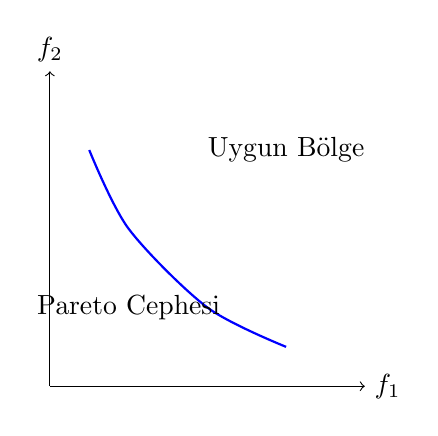
\begin{tikzpicture}
\draw[->] (0,0) -- (4,0) node[right] {$f_1$};
\draw[->] (0,0) -- (0,4) node[above] {$f_2$};
\draw[blue,thick] plot[smooth] coordinates {(0.5,3) (1,2) (2,1) (3,0.5)};
\node at (3,3) {Uygun Bölge};
\node at (1,1) {Pareto Cephesi};
\end{tikzpicture}
\caption{Pareto cephesi örneği}
\end{marginfigure}

\subsection{Çözüm Yaklaşımları}
Çok amaçlı optimizasyon problemlerinin çözümünde kullanılan temel stratejilerin incelenmesi, problemi ele alış biçimine göre farklı yaklaşımlar sunar. Yani esas olarak burada karar verici mühendisin kendisidir. Amaç fonksiyonlarının birbirlerine kıyasla üstün olup olmaması veya oransallığı bu kararda ve seçilecek stratejide etkilidir.

\subsubsection{Skalerleştirme Yöntemleri}
Çok amaçlı optimizasyon problemini tek amaçlı probleme dönüştüren yaklaşımlardır. Bu yöntemler, çoklu amaçları birleştirerek problemi daha kolay çözülebilir hale getirir. Skalerleştirme yöntemleri, hızlı ve kolay uygulanabilir olmaları nedeniyle mühendislik problemlerinde yaygın olarak kullanılır. Ancak uygun ağırlıkların belirlenmesi, çözümün kalitesini doğrudan etkilediği için süreci zorlaştırabilir.

\begin{tcolorbox}[title=Yaygın Skalerleştirme Yöntemleri]
\begin{itemize}
    \item \textbf{Ağırlıklı Toplam Yöntemi:} $F(x) = \sum_{i=1}^{k} w_i f_i(x)$
    \item \textbf{$\varepsilon$-Kısıt Yöntemi:} Bir amaç optimize edilirken diğerleri kısıt olarak tanımlanır
    \item \textbf{Hedef Programlama:} $\min \sum_{i=1}^{k} w_i |f_i(x) - T_i|$ (burada $T_i$ hedef değerlerdir)
\end{itemize}
\end{tcolorbox}

\subsubsection{Pareto Tabanlı Yaklaşımlar}
Pareto tabanlı yaklaşımlar, tüm Pareto-optimal çözümleri veya bunların iyi bir temsilini bulmayı hedefler. Bu yöntemler, çözüm uzayının daha geniş bir bölümünü keşfetmeyi sağlar ve karar vericiye daha fazla alternatif sunar. Pareto tabanlı yaklaşımlar, özellikle evrimsel algoritmaların kullanıldığı durumlarda daha etkilidir.

Pareto tabanlı yaklaşımların temel bileşenleri şunlardır:
\begin{itemize}
    \item \textbf{Baskınlık İlişkisi:} Bir çözümün diğerine göre daha iyi olup olmadığının belirlenmesi
    \item \textbf{Çeşitlilik Mekanizmaları:} Pareto cephesi boyunca çözümlerin homojen dağılmasını sağlayan teknikler
    \item \textbf{Elit Stratejiler:} İyi çözümlerin korunmasını sağlayan mekanizmalar
\end{itemize}

\begin{marginfigure}
\centering
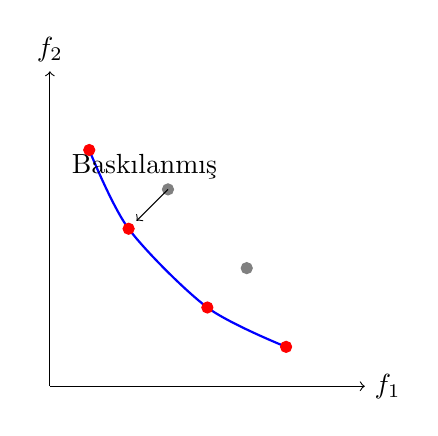
\begin{tikzpicture}
\draw[->] (0,0) -- (4,0) node[right] {$f_1$};
\draw[->] (0,0) -- (0,4) node[above] {$f_2$};
\draw[blue,thick] plot[smooth] coordinates {(0.5,3) (1,2) (2,1) (3,0.5)};
\filldraw[red] (0.5,3) circle (2pt);
\filldraw[red] (1,2) circle (2pt);
\filldraw[red] (2,1) circle (2pt);
\filldraw[red] (3,0.5) circle (2pt);
\filldraw[gray] (1.5,2.5) circle (2pt);
\filldraw[gray] (2.5,1.5) circle (2pt);
\draw[->] (1.5,2.5) -- (1.1,2.1);
\node at (1.2,2.8) {Baskılanmış};
\end{tikzpicture}
\caption{Pareto baskınlık kavramı}
\end{marginfigure}

\subsubsection{İnteraktif Yöntemler}
İnteraktif yöntemler, karar vericiyi optimizasyon sürecine dahil ederek, tercihlerine göre çözüm uzayını daraltır. Bu yaklaşım, karar vericinin bilgi ve deneyimini algoritmanın çalışmasına entegre eder. İnteraktif yöntemler, özellikle karmaşık mühendislik problemlerinde, uzman bilgisinin çözüm sürecine dahil edilmesi açısından değerlidir.

İnteraktif yaklaşımların avantajları:
\begin{itemize}
    \item Karar vericinin tercihlerini doğrudan sürece yansıtabilme
    \item Hesaplama kaynaklarını ilgi duyulan çözüm bölgesine yönlendirme
    \item Daha anlamlı ve uygulanabilir sonuçlar elde etme
\end{itemize}

\subsection{Evrimsel Çok Amaçlı Optimizasyon Algoritmaları}
Evrimsel algoritmaların çok amaçlı optimizasyon problemlerine uygulanması, klasik yöntemlere göre önemli avantajlar sağlar. Bu algoritmalar, tek seferde birden fazla çözüm üretebilme, karmaşık amaç fonksiyonlarını ele alabilme ve geniş çözüm uzaylarını etkili bir şekilde tarayabilme özellikleriyle öne çıkar.

\subsubsection{NSGA-II (Non-dominated Sorting Genetic Algorithm)}
NSGA-II, çok amaçlı evrimsel optimizasyon alanında en yaygın kullanılan algoritmalardan biridir. Baskınlık sıralama ve yoğunluk mesafesi hesaplama mekanizmalarıyla, hem Pareto-optimal çözümlere yakınsama hem de çözümler arasında çeşitlilik sağlar. NSGA-II, $O(MN^2)$ hesaplama karmaşıklığıyla oldukça verimli çalışır ve birçok mühendislik probleminde başarıyla uygulanmıştır.

NSGA-II'nin temel bileşenleri:
\begin{itemize}
    \item \textbf{Hızlı Baskınlık Sıralama:} Popülasyondaki çözümleri baskınlık ilişkisine göre sıralar
    \item \textbf{Yoğunluk Mesafesi:} Aynı baskınlık seviyesindeki çözümler arasında çeşitliliği korur
    \item \textbf{İkili Turnuva Seçimi:} Baskınlık seviyesi ve yoğunluk mesafesine dayalı seçim mekanizması
\end{itemize}


\subsubsection{MOEA/D (Multiobjective Evolutionary Algorithm based on Decomposition)}
MOEA/D, çok amaçlı optimizasyon problemini bir dizi tek amaçlı alt probleme ayrıştırarak çözen bir evrimsel algoritmadır. Her alt problem, komşu alt problemlerle bilgi paylaşımı yaparak eş zamanlı olarak optimize edilir. Bu yaklaşım, özellikle çok sayıda amaç fonksiyonu içeren problemlerde etkilidir ve hesaplama açısından verimlidir.

MOEA/D'nin avantajları:
\begin{itemize}
    \item Komşuluk yapısı sayesinde etkili bilgi paylaşımı
    \item Çok sayıda amaç fonksiyonu içeren problemlere uygunluk
    \item Farklı ayrıştırma yöntemlerinin kullanılabilmesi (Tchebycheff, ağırlıklı toplam vb.)
\end{itemize}

\subsubsection{SPEA2 (Strength Pareto Evolutionary Algorithm)}
SPEA2, sabit büyüklükte bir arşiv kullanarak Pareto-optimal çözümleri saklayan ve rafine eden bir evrimsel algoritmadır. Algoritma, her çözüme bir uygunluk değeri atayarak hem baskınlık ilişkisini hem de çözüm yoğunluğunu dikkate alır. SPEA2, özellikle çeşitlilik ve yakınsama arasında iyi bir denge kurması nedeniyle tercih edilir.

SPEA2'nin önemli özellikleri:
\begin{itemize}
    \item \textbf{Güç Değeri:} Bir çözümün kaç çözümü baskıladığını ölçer
    \item \textbf{Yoğunluk Tahmini:} K-en yakın komşu yöntemiyle hesaplanır
    \item \textbf{Harici Arşiv:} Pareto-optimal çözümleri etkin bir şekilde depolar ve günceller
\end{itemize}

\subsection{Karar Verme Süreçleri}
Çok amaçlı optimizasyon, bir dizi Pareto-optimal çözüm üretir ve bu çözümler arasından seçim yapılması gerekir. Karar verme süreci, optimizasyon sürecinin kritik bir parçasıdır ve çeşitli yaklaşımlarla desteklenebilir.

\subsubsection{Çözüm Seçimi Kriterleri}
Pareto-optimal çözümler arasından seçim yaparken kullanılabilecek çeşitli kriterler vardır:
\begin{itemize}
    \item \textbf{Uzaklık Ölçüleri:} İdeal noktaya en yakın çözüm (örn. Öklid mesafesi, Tchebycheff mesafesi)
    \item \textbf{Tatmin Düzeyi:} Her amaç için belirlenen eşik değerlerini sağlayan çözümler
    \item \textbf{Göreceli İyileştirme:} Bir amacın diğerine göre iyileşme oranı (trade-off analizi)
    \item \textbf{Risk Analizi:} Belirsizlik altında çözümlerin güvenilirliği
\end{itemize}

\begin{tcolorbox}[title=Örnek: Ağırlıklı Tchebycheff Metriği]
\begin{equation}
d(F, F^*) = \max_{i=1,...,k} \{w_i \cdot |F_i - F_i^*|\}
\end{equation}
Burada $F^*$ ideal nokta, $w_i$ amaçların ağırlıkları, $F_i$ mevcut çözümün $i$. amaç değeridir.
\end{tcolorbox}

\subsubsection{Ağırlıklandırma Stratejileri}
Amaçların göreceli önemini belirlemek için çeşitli ağırlıklandırma stratejileri kullanılabilir:
\begin{itemize}
    \item \textbf{Doğrudan Atama:} Karar vericinin doğrudan ağırlık ataması
    \item \textbf{AHP (Analitik Hiyerarşi Süreci):} İkili karşılaştırmalar yoluyla ağırlık belirleme
    \item \textbf{Entropi Tabanlı Yöntemler:} Veri dağılımına göre ağırlık hesaplama
    \item \textbf{TOPSIS:} İdeal çözüme benzerlik ile ağırlıklandırma
\end{itemize}

\subsubsection{Çözümler Arası Kıyaslama}
Farklı Pareto-optimal çözümlerin karşılaştırılması, karar vericinin tercihine uygun çözümü seçmesine yardımcı olur:
\begin{itemize}
    \item \textbf{Görselleştirme Teknikleri:} Paralel koordinat grafikleri, yıldız diyagramları, ısı haritaları
    \item \textbf{Duyarlılık Analizi:} Parametrelerdeki değişimlerin çözüme etkisi
    \item \textbf{Robust Değerlendirme:} Belirsizlik altında çözümlerin performansı
    \item \textbf{Yaşam Döngüsü Analizi:} Uzun vadeli performans ve maliyet değerlendirmesi
\end{itemize}

\begin{marginfigure}
\centering
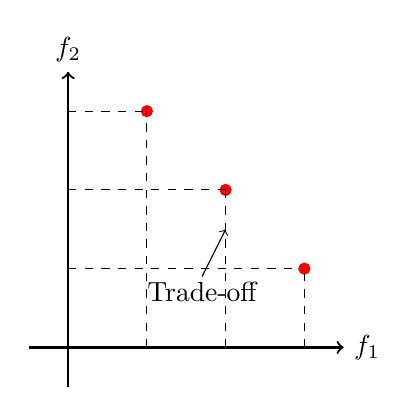
\begin{tikzpicture}
\draw[->,thick] (-0.5,0) -- (3.5,0) node[right] {$f_1$};
\draw[->,thick] (0,-0.5) -- (0,3.5) node[above] {$f_2$};
\filldraw[red] (1,3) circle (2pt);
\filldraw[red] (2,2) circle (2pt);
\filldraw[red] (3,1) circle (2pt);
\draw[dashed] (1,0) -- (1,3);
\draw[dashed] (0,3) -- (1,3);
\draw[dashed] (2,0) -- (2,2);
\draw[dashed] (0,2) -- (2,2);
\draw[dashed] (3,0) -- (3,1);
\draw[dashed] (0,1) -- (3,1);
\node at (1.7,0.7) {Trade-off};
\draw[->] (1.7,0.9) -- (2,1.5);
\end{tikzpicture}
\caption{Pareto çözümleri arasındaki trade-off analizi}
\end{marginfigure}


\subsection{Çok Amaçlı Optimizasyonda Performans Metrikleri}
\subsubsection{Hypervolume (Hiperhaciim)}
Hiperhacim, çok amaçlı optimizasyon algoritmalarının performansını değerlendirmek için kullanılan en yaygın metriklerden biridir. Bu metrik, Pareto cephesinin referans noktasına göre kapladığı alanın veya hacmin ölçüsünü ifade eder. Daha yüksek hiperhacim değeri, algoritmanın daha iyi bir Pareto cephesi bulduğunu gösterir, çünkü bu durum çözüm uzayının daha geniş bir bölümünün kapsandığını ifade eder.

\subsubsection{IGD (Ters Nesil Mesafesi)}
Ters Nesil Mesafesi (IGD), gerçek Pareto cephesi ile algoritma tarafından bulunan çözüm kümesi arasındaki mesafenin bir ölçüsüdür. Bu metrik, bulunan çözümlerin gerçek Pareto cephesine ne kadar yakın olduğunu ve cepheyi ne kadar iyi temsil ettiğini gösterir. Daha düşük IGD değeri, algoritmanın gerçek Pareto cephesine daha yakın ve daha iyi dağılmış çözümler bulduğunu ifade eder.

\subsubsection{Yayılım (Çeşitlilik)}
Yayılım metriği, çözüm kümesindeki noktaların birbirlerine olan uzaklığının ölçüsüdür ve Pareto cephesi boyunca çözümlerin ne kadar homojen dağıldığını gösterir. Bu metrik, algoritmanın çözüm uzayını ne kadar iyi keşfettiğini ve çeşitli alternatifler sunabildiğini değerlendirir. Düzgün dağılmış bir Pareto cephesi için daha düşük yayılım değerleri tercih edilir.

\subsubsection{Hesaplama Süresi}
Hesaplama süresi, bir algoritmanın çözüme ulaşmak için harcadığı zamanı ölçer. Bu metrik, algoritmanın verimliliğini ve pratik uygulamalardaki kullanılabilirliğini değerlendirmek için önemlidir. Özellikle karmaşık mühendislik problemlerinde, makul bir sürede iyi sonuçlar verebilen algoritmalar tercih edilir. Hesaplama süresi, algoritmanın karmaşıklığına, problem boyutuna ve uygulama ortamına bağlı olarak değişebilir. \sidenote{Bu parametre oldukça bağıl olması sebebiyle, her zaman güvenilir sonuçlar vermez. Günümüzde CPU Time gibi daha modern metrikler kullanılır.}  
\section{Application I}
This section will demonstrate the size optimization of a cantilever beam consisting of five different parts.

\sidenote{
    
\qrcode[height=1in]{https://github.com/btayfur/structural-optimization/blob/main/Code/Examples/Exmp6/}}

\subsection{Problem Definition}
In this application, an optimization problem aiming to minimize the weight of a 3-meter-long cantilever beam divided into 5 equal parts will be addressed. The details of the problem are as follows:

\begin{itemize}
    \item A 3-meter-long cantilever beam divided into 5 equal parts
    \item Each part has a hollow circular cross-section with two design parameters:
    \begin{itemize}
        \item $r_{outer}$: Outer radius
        \item $r_{inner}$: Inner radius
    \end{itemize}
    \item Material: S270 steel (E = 210 GPa, $\sigma_y$ = 270 MPa)
    \item A force F = 500 kN is applied perpendicular to the free end of the beam
    \item Objective: Minimize the weight of the beam
\end{itemize}

\subsubsection{Constraints}
\begin{enumerate}
    \item A maximum displacement of 2 cm is allowed at the free end of the beam
    \item For each part, the outer radius must be greater than the inner radius
    \item The inner radius of the previous part must be smaller than the outer radius of the next part (weldability condition)
    \item The yield stress of S270 steel (270 MPa) must not be exceeded
\end{enumerate}

\subsection{Structural Analysis}
The finite element method has been used for displacement and stress analysis of the cantilever beam:

\begin{itemize}
    \item Each beam part is modeled as an Euler-Bernoulli beam element
    \item Each node has 2 degrees of freedom (displacement and rotation)
    \item Global stiffness matrix is created to calculate displacements
    \item Stresses are calculated using bending moment and section properties
\end{itemize}

\subsubsection{Stiffness Matrix Formation}
The stiffness matrix for the beam element is formed as follows:

\begin{equation}
k_e = \begin{bmatrix}
\frac{12EI}{l^3} & \frac{6EI}{l^2} & -\frac{12EI}{l^3} & \frac{6EI}{l^2} \\
\frac{6EI}{l^2} & \frac{4EI}{l} & -\frac{6EI}{l^2} & \frac{2EI}{l} \\
-\frac{12EI}{l^3} & -\frac{6EI}{l^2} & \frac{12EI}{l^3} & -\frac{6EI}{l^2} \\
\frac{6EI}{l^2} & \frac{2EI}{l} & -\frac{6EI}{l^2} & \frac{4EI}{l}
\end{bmatrix}
\end{equation}

Where:
\begin{itemize}
    \item $E$: Young's modulus
    \item $I$: Moment of inertia
    \item $l$: Element length
\end{itemize}

Moment of inertia for hollow circular cross-section:
\begin{equation}
I = \frac{\pi}{4}(r_{outer}^4 - r_{inner}^4)
\end{equation}

\subsubsection{Boundary Conditions and Solution}
The left end of the cantilever beam is fixed, therefore the degrees of freedom at the first node are zero. The force applied to the right end is added to the global force vector. The displacement vector is solved using the reduced stiffness matrix and force vector:

\begin{equation}
\mathbf{K_{reduced}} \cdot \mathbf{u} = \mathbf{F}
\end{equation}

\subsection{Optimization Approach}
The Simulated Annealing algorithm has been used for optimization:

\begin{itemize}
    \item Random search strategy to avoid local optima
    \item Adaptive step size for effective exploration of solution space
    \item Slow cooling of process temperature to find better solutions
    \item Effective control of constraints to ensure physically feasible solutions
\end{itemize}

\subsubsection{Objective Function}
The objective function is the total weight of the beam:

\begin{equation}
W = \rho \sum_{i=1}^{5} A_i \cdot l_i
\end{equation}

Where:
\begin{itemize}
    \item $\rho$: Material density
    \item $A_i$: Cross-sectional area of each part ($A_i = \pi(r_{outer,i}^2 - r_{inner,i}^2)$)
    \item $l_i$: Length of each part
\end{itemize}

\subsubsection{Constraint Functions}
Four constraint functions are used in the optimization process:

\begin{enumerate}
    \item Displacement constraint: $u_{max} \leq 0.02$ m
    \item Radius constraint: $r_{outer,i} > r_{inner,i}$ (for each part)
    \item Weldability constraint: $r_{inner,i} < r_{outer,i+1}$ (for adjacent parts)
    \item Stress constraint: $\sigma_{max} \leq \sigma_{yield}$
\end{enumerate}

\subsection{Optimization Results}
The optimization resulted in a lighter beam design compared to the initial design:

\begin{itemize}
    \item Initial design weight: $\sim$1924 kg
    \item Optimized design weight: $\sim$939 kg (51\% reduction)
\end{itemize}

\begin{figure}[H]
    \centering
    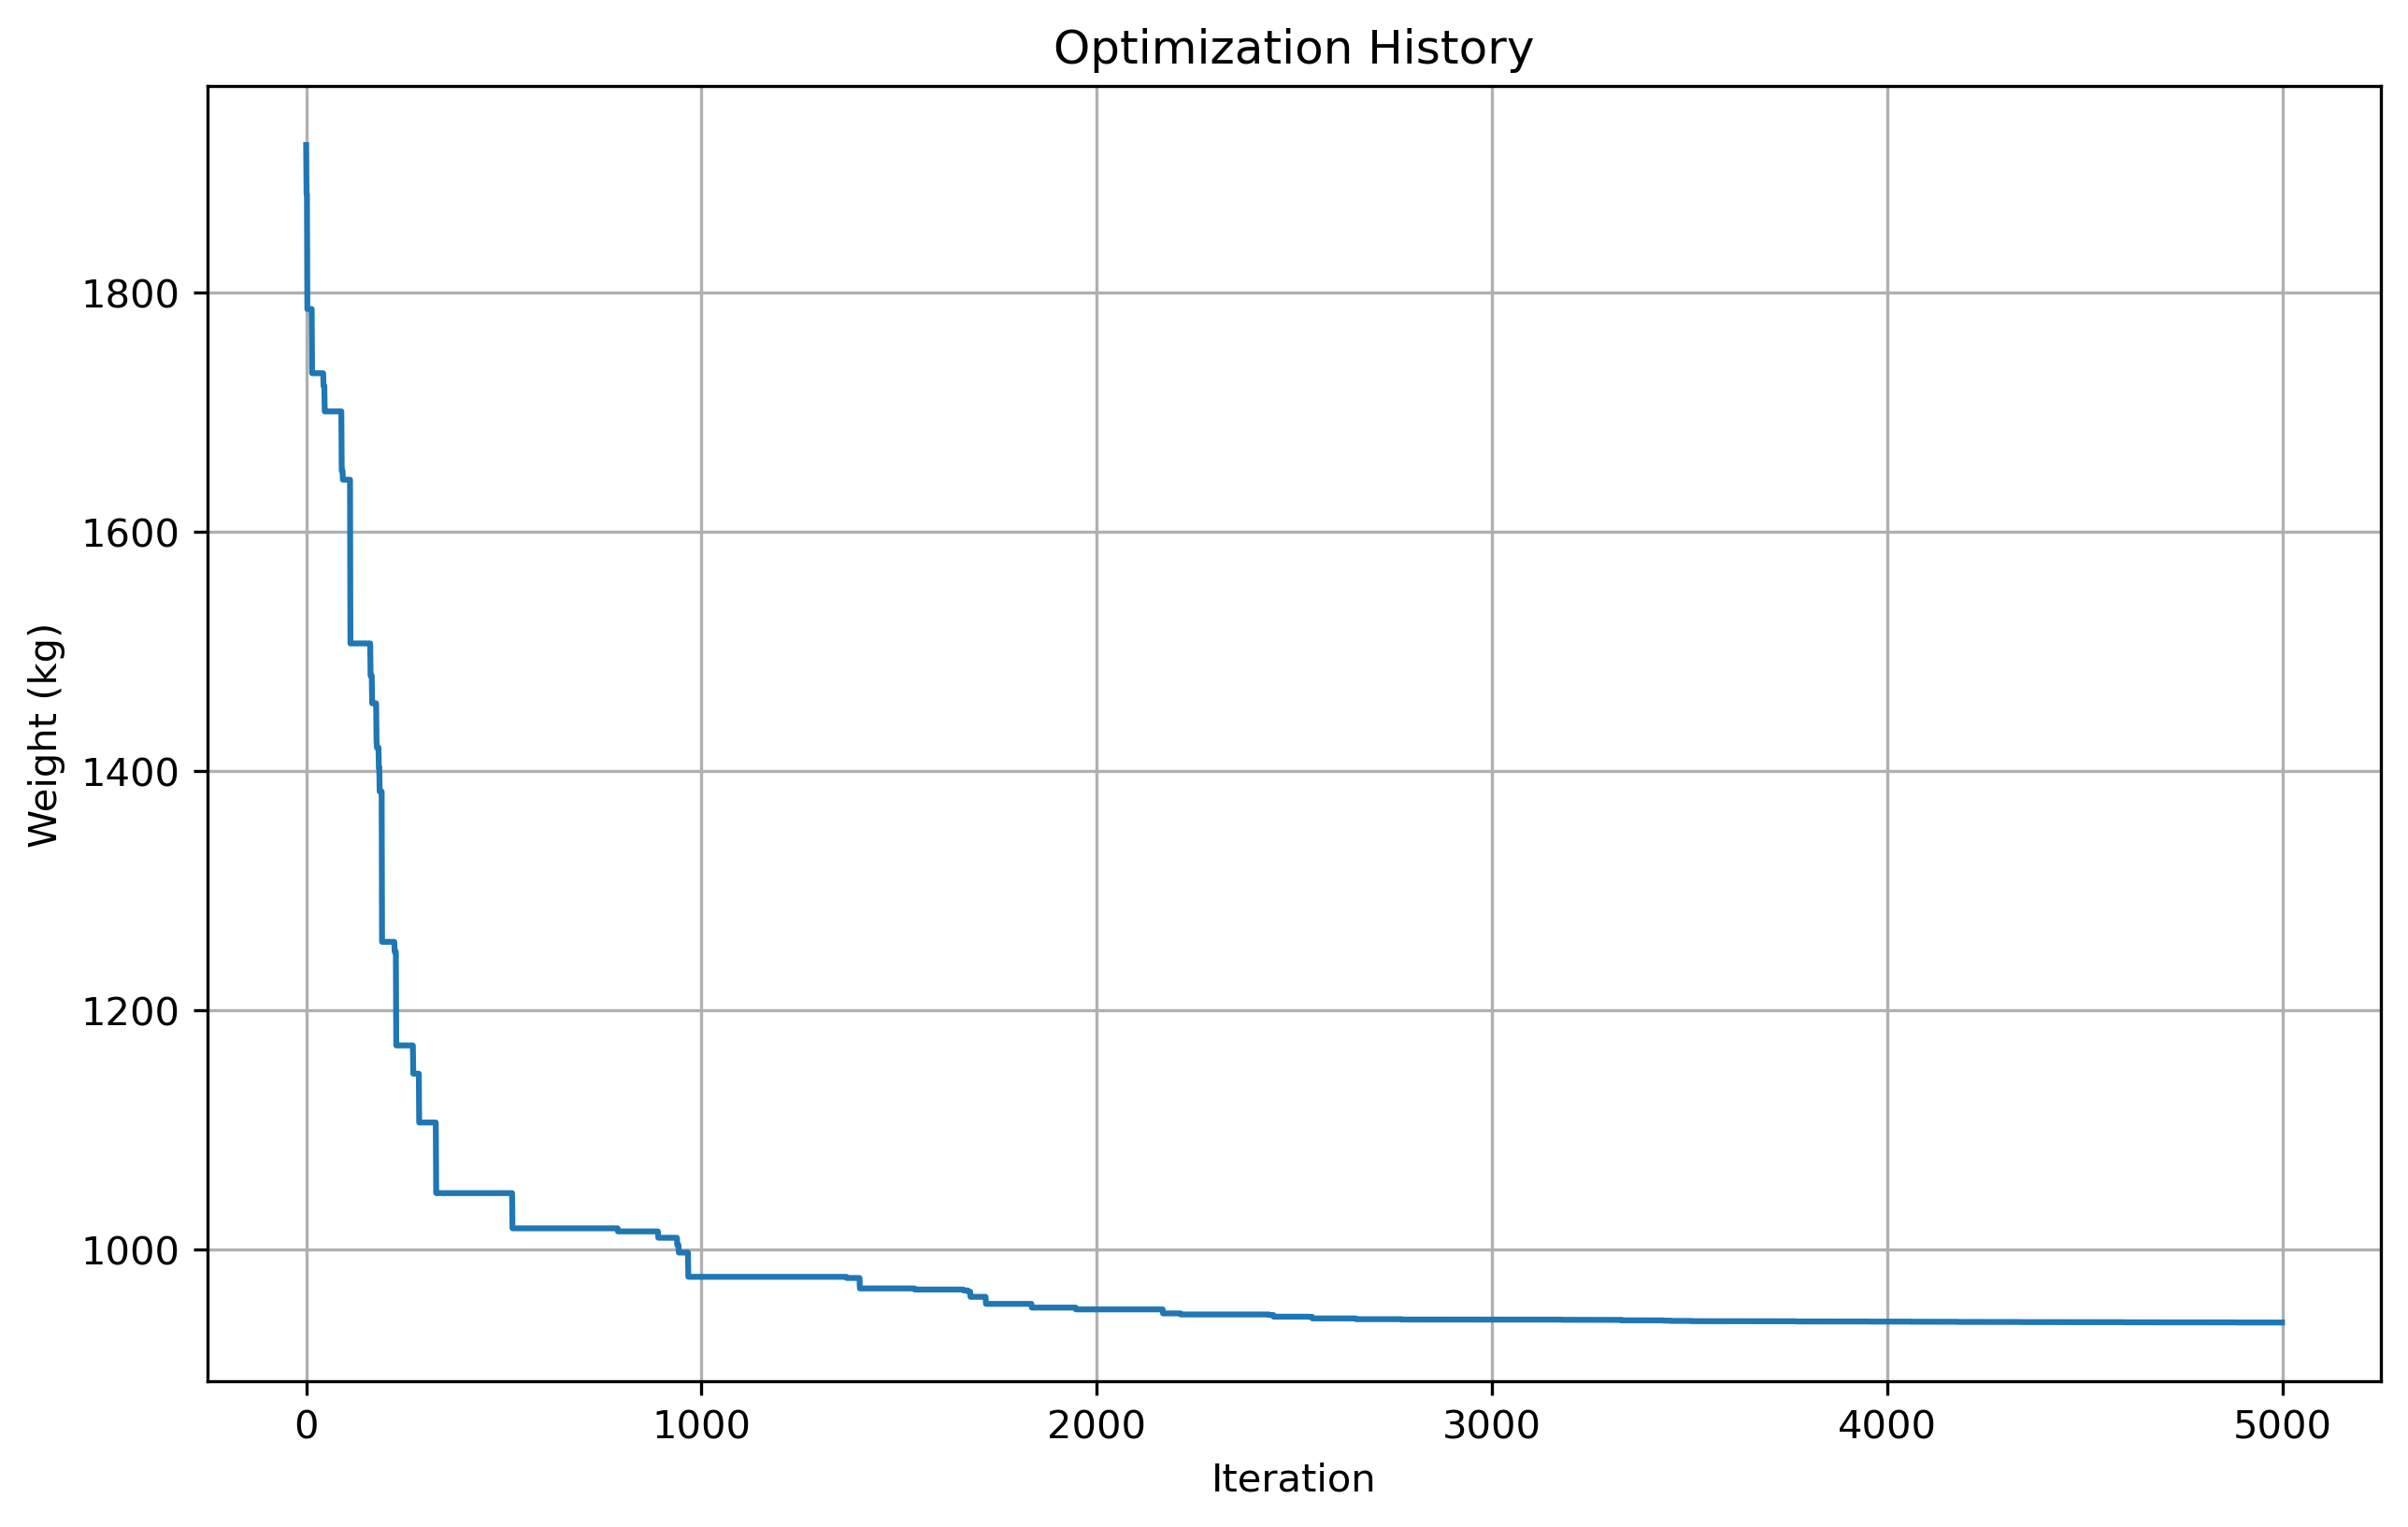
\includegraphics[width=1\textwidth]{weeks_new/imgs/optimization_history.png}
    \caption{Weight Tracking Graph}
    \label{fig:optimization_history}
\end{figure}

\subsubsection{Optimized Radii (cm)}
\begin{center}
\begin{tabular}{|c|c|c|}
\hline
Part & Outer Radius ($r_{outer}$) & Inner Radius ($r_{inner}$) \\
\hline
1 & 20.37 & 14.36 \\
2 & 20.05 & 15.81 \\
3 & 15.82 & 9.04 \\
4 & 16.00 & 13.33 \\
5 & 14.26 & 13.30 \\
\hline
\end{tabular}
\end{center}

In the optimized design:
\begin{itemize}
    \item The displacement at the end point is 0.12 cm (maximum allowed 2 cm)
    \item The stress constraint is active (0.00 MPa margin)
    \item The cross-section dimensions satisfy the weldability condition
\end{itemize}

\subsubsection{Optimized Beam Design}
The geometry of the optimized beam shows that the cross-section dimensions decrease from the support point (left side) towards the free end. This is consistent with the bending moment being maximum at the support and decreasing towards the free end.
\begin{figure}[H]
    \centering
    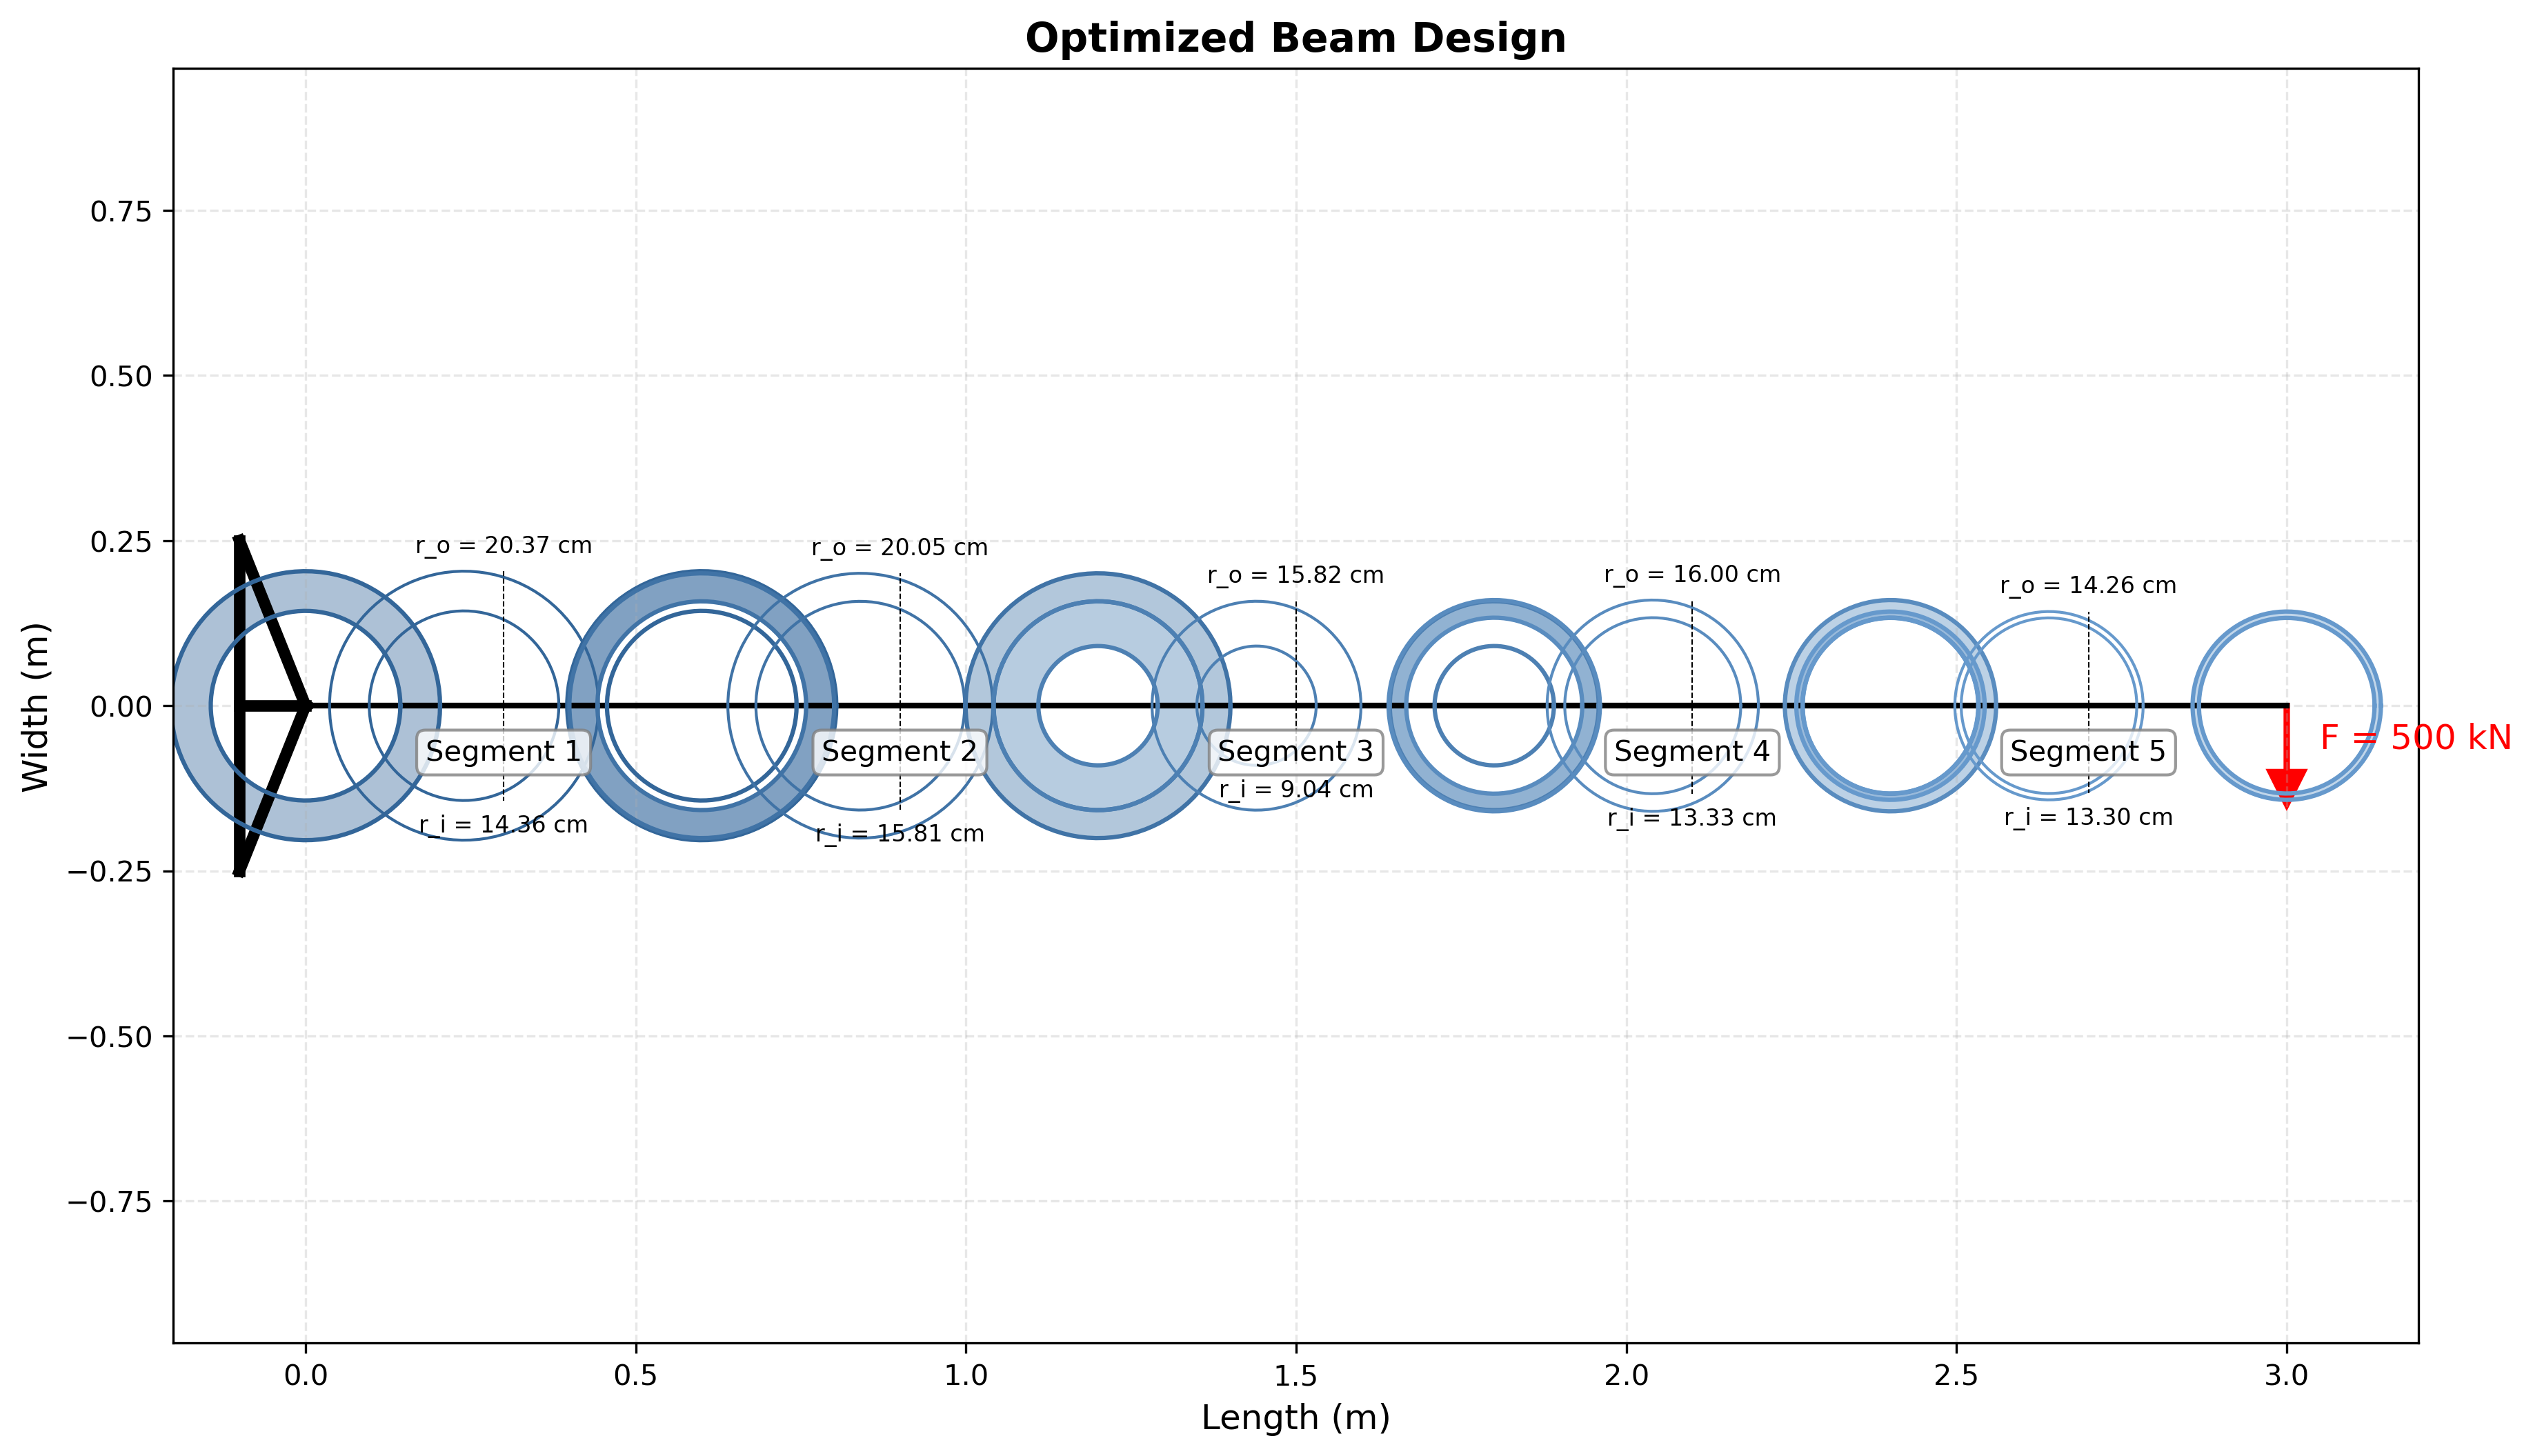
\includegraphics[width=1\textwidth]{weeks_new/imgs/optimized_beam.png}
    \caption{Optimized Beam Design}
    \label{fig:optimized_beam}
\end{figure}

\subsubsection{Deformation Shape}
The deformation shape of the cantilever beam under load has a maximum displacement of 2 cm at the free end. The displacement values at each node are also shown.

\begin{figure}[H]
    \centering
    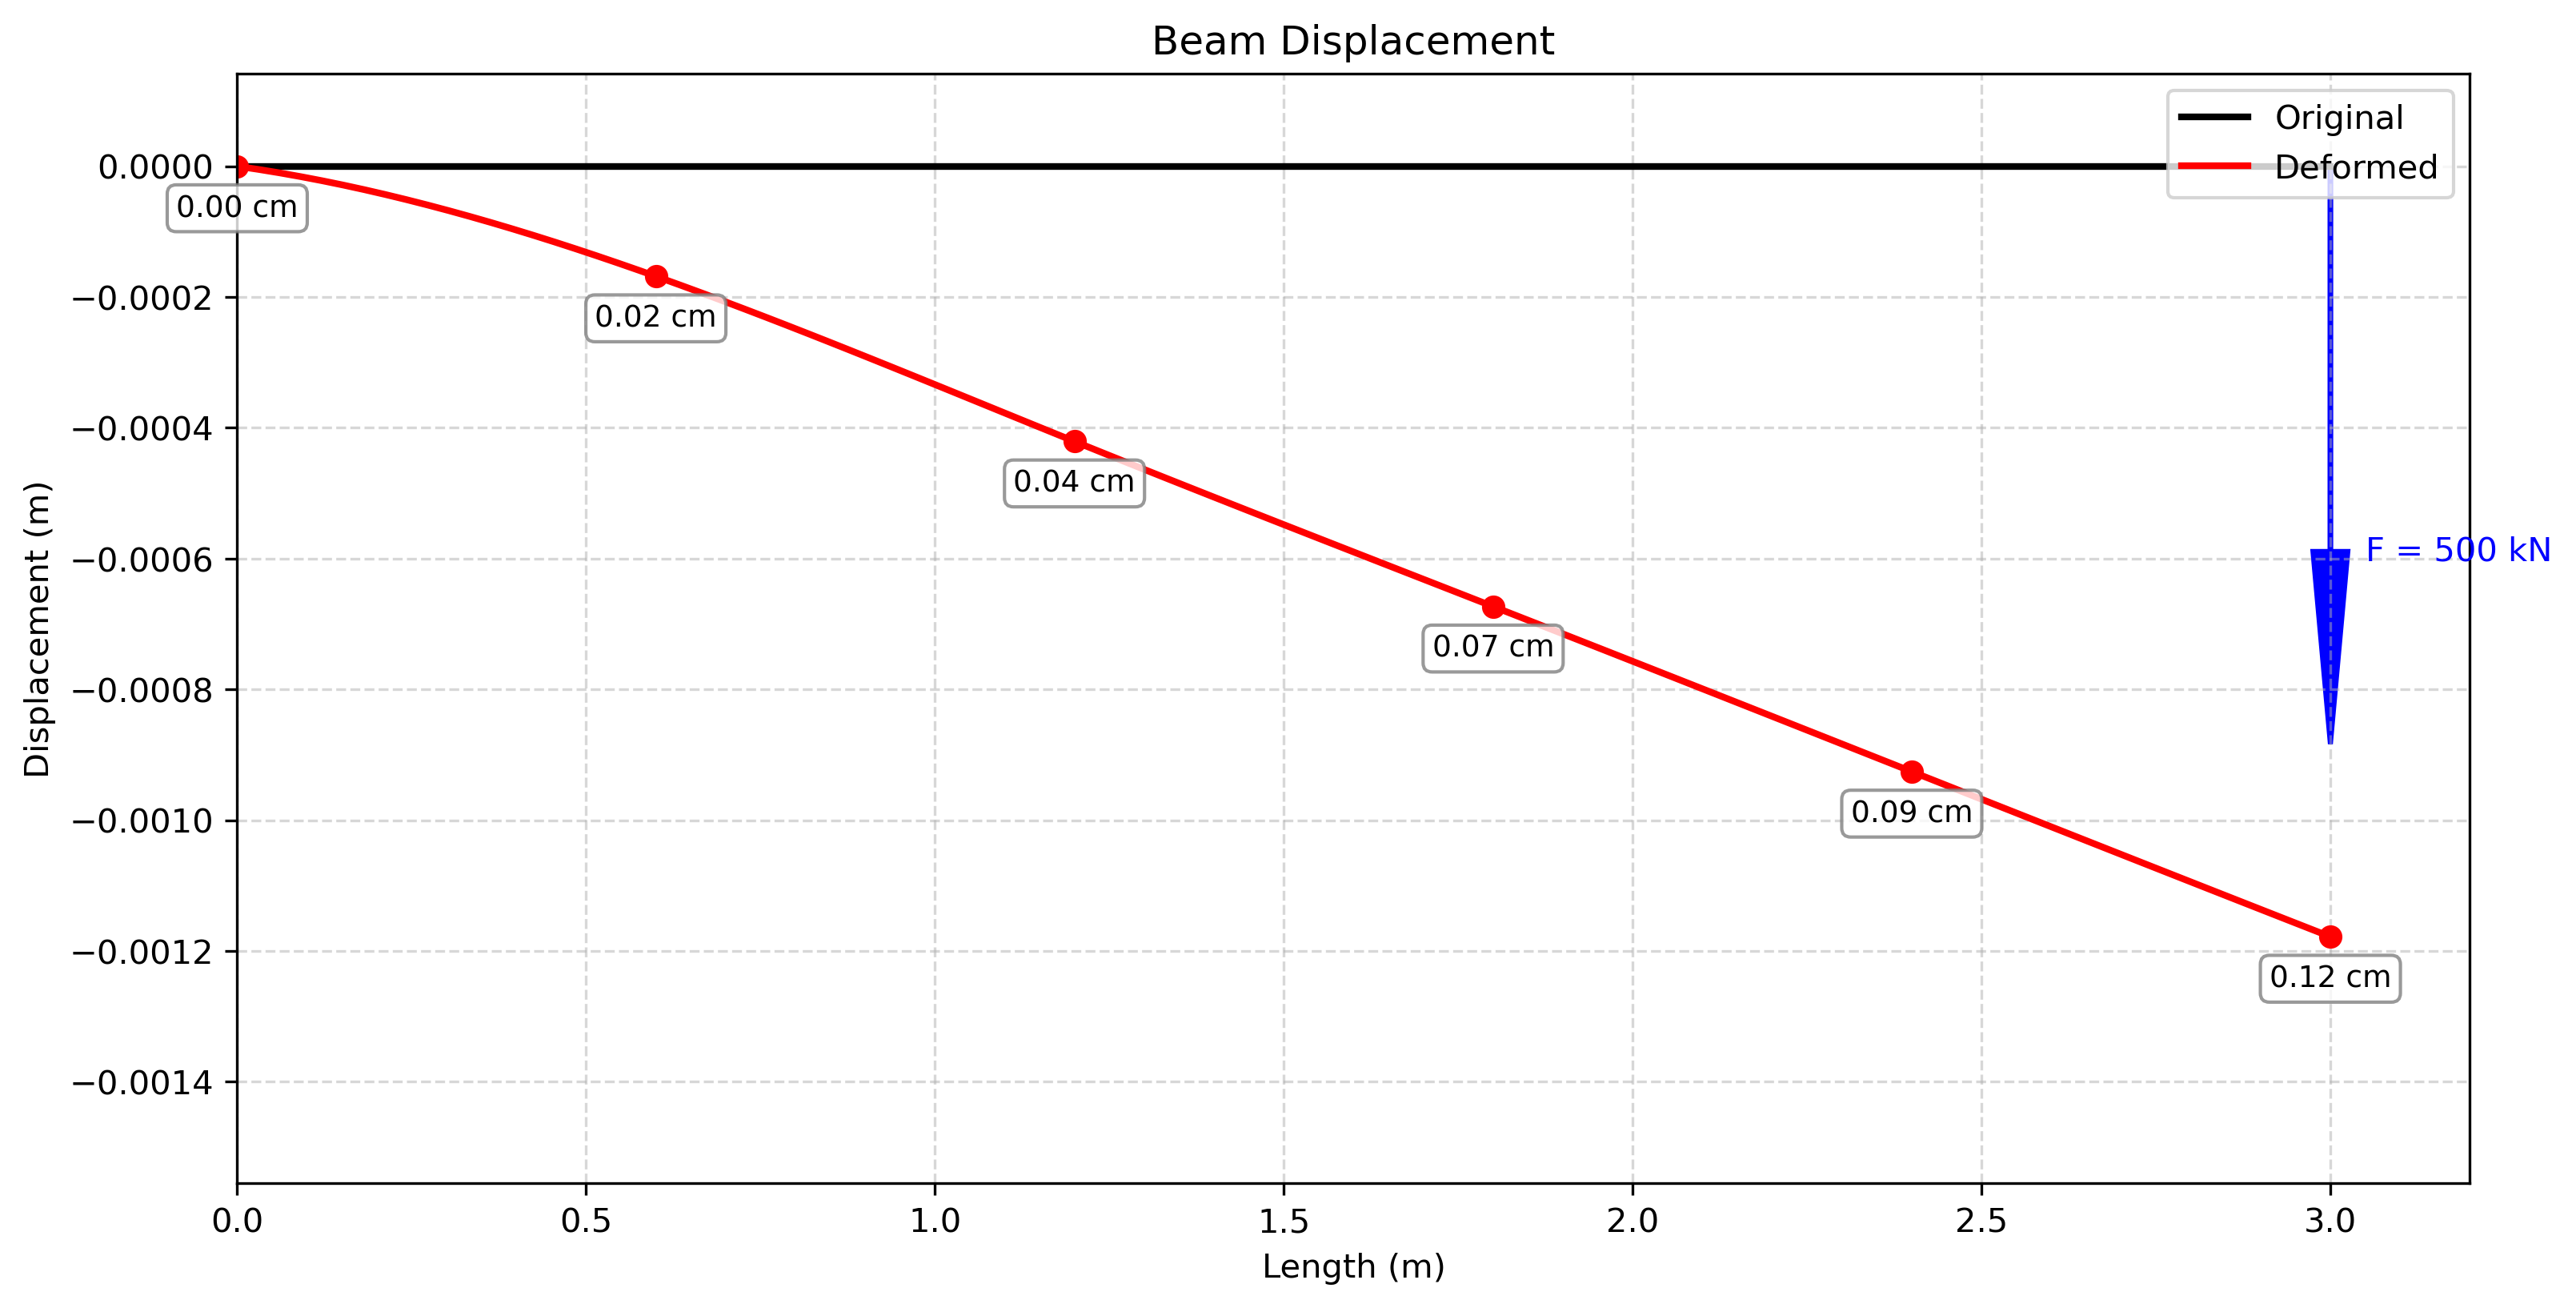
\includegraphics[width=1\textwidth]{weeks_new/imgs/deformed_beam.png}
    \caption{Deformation Shape}
    \label{fig:deformed_beam}
\end{figure}

\subsubsection{Constraint Utilization Ratios}
Graphs have been created showing how much each constraint is utilized in the optimized design:

\begin{itemize}
    \item \textbf{Displacement Constraint:} Maximum displacement limit is fully utilized (100\%)
    \item \textbf{Stress Constraint:} Yield stress utilization ratio for each segment
    \item \textbf{Radius Ratio:} Ratio of inner radius to outer radius
    \item \textbf{Weldability:} Utilization ratio of the welding condition between adjacent segments
\end{itemize}

\begin{figure}[H]
    \centering
    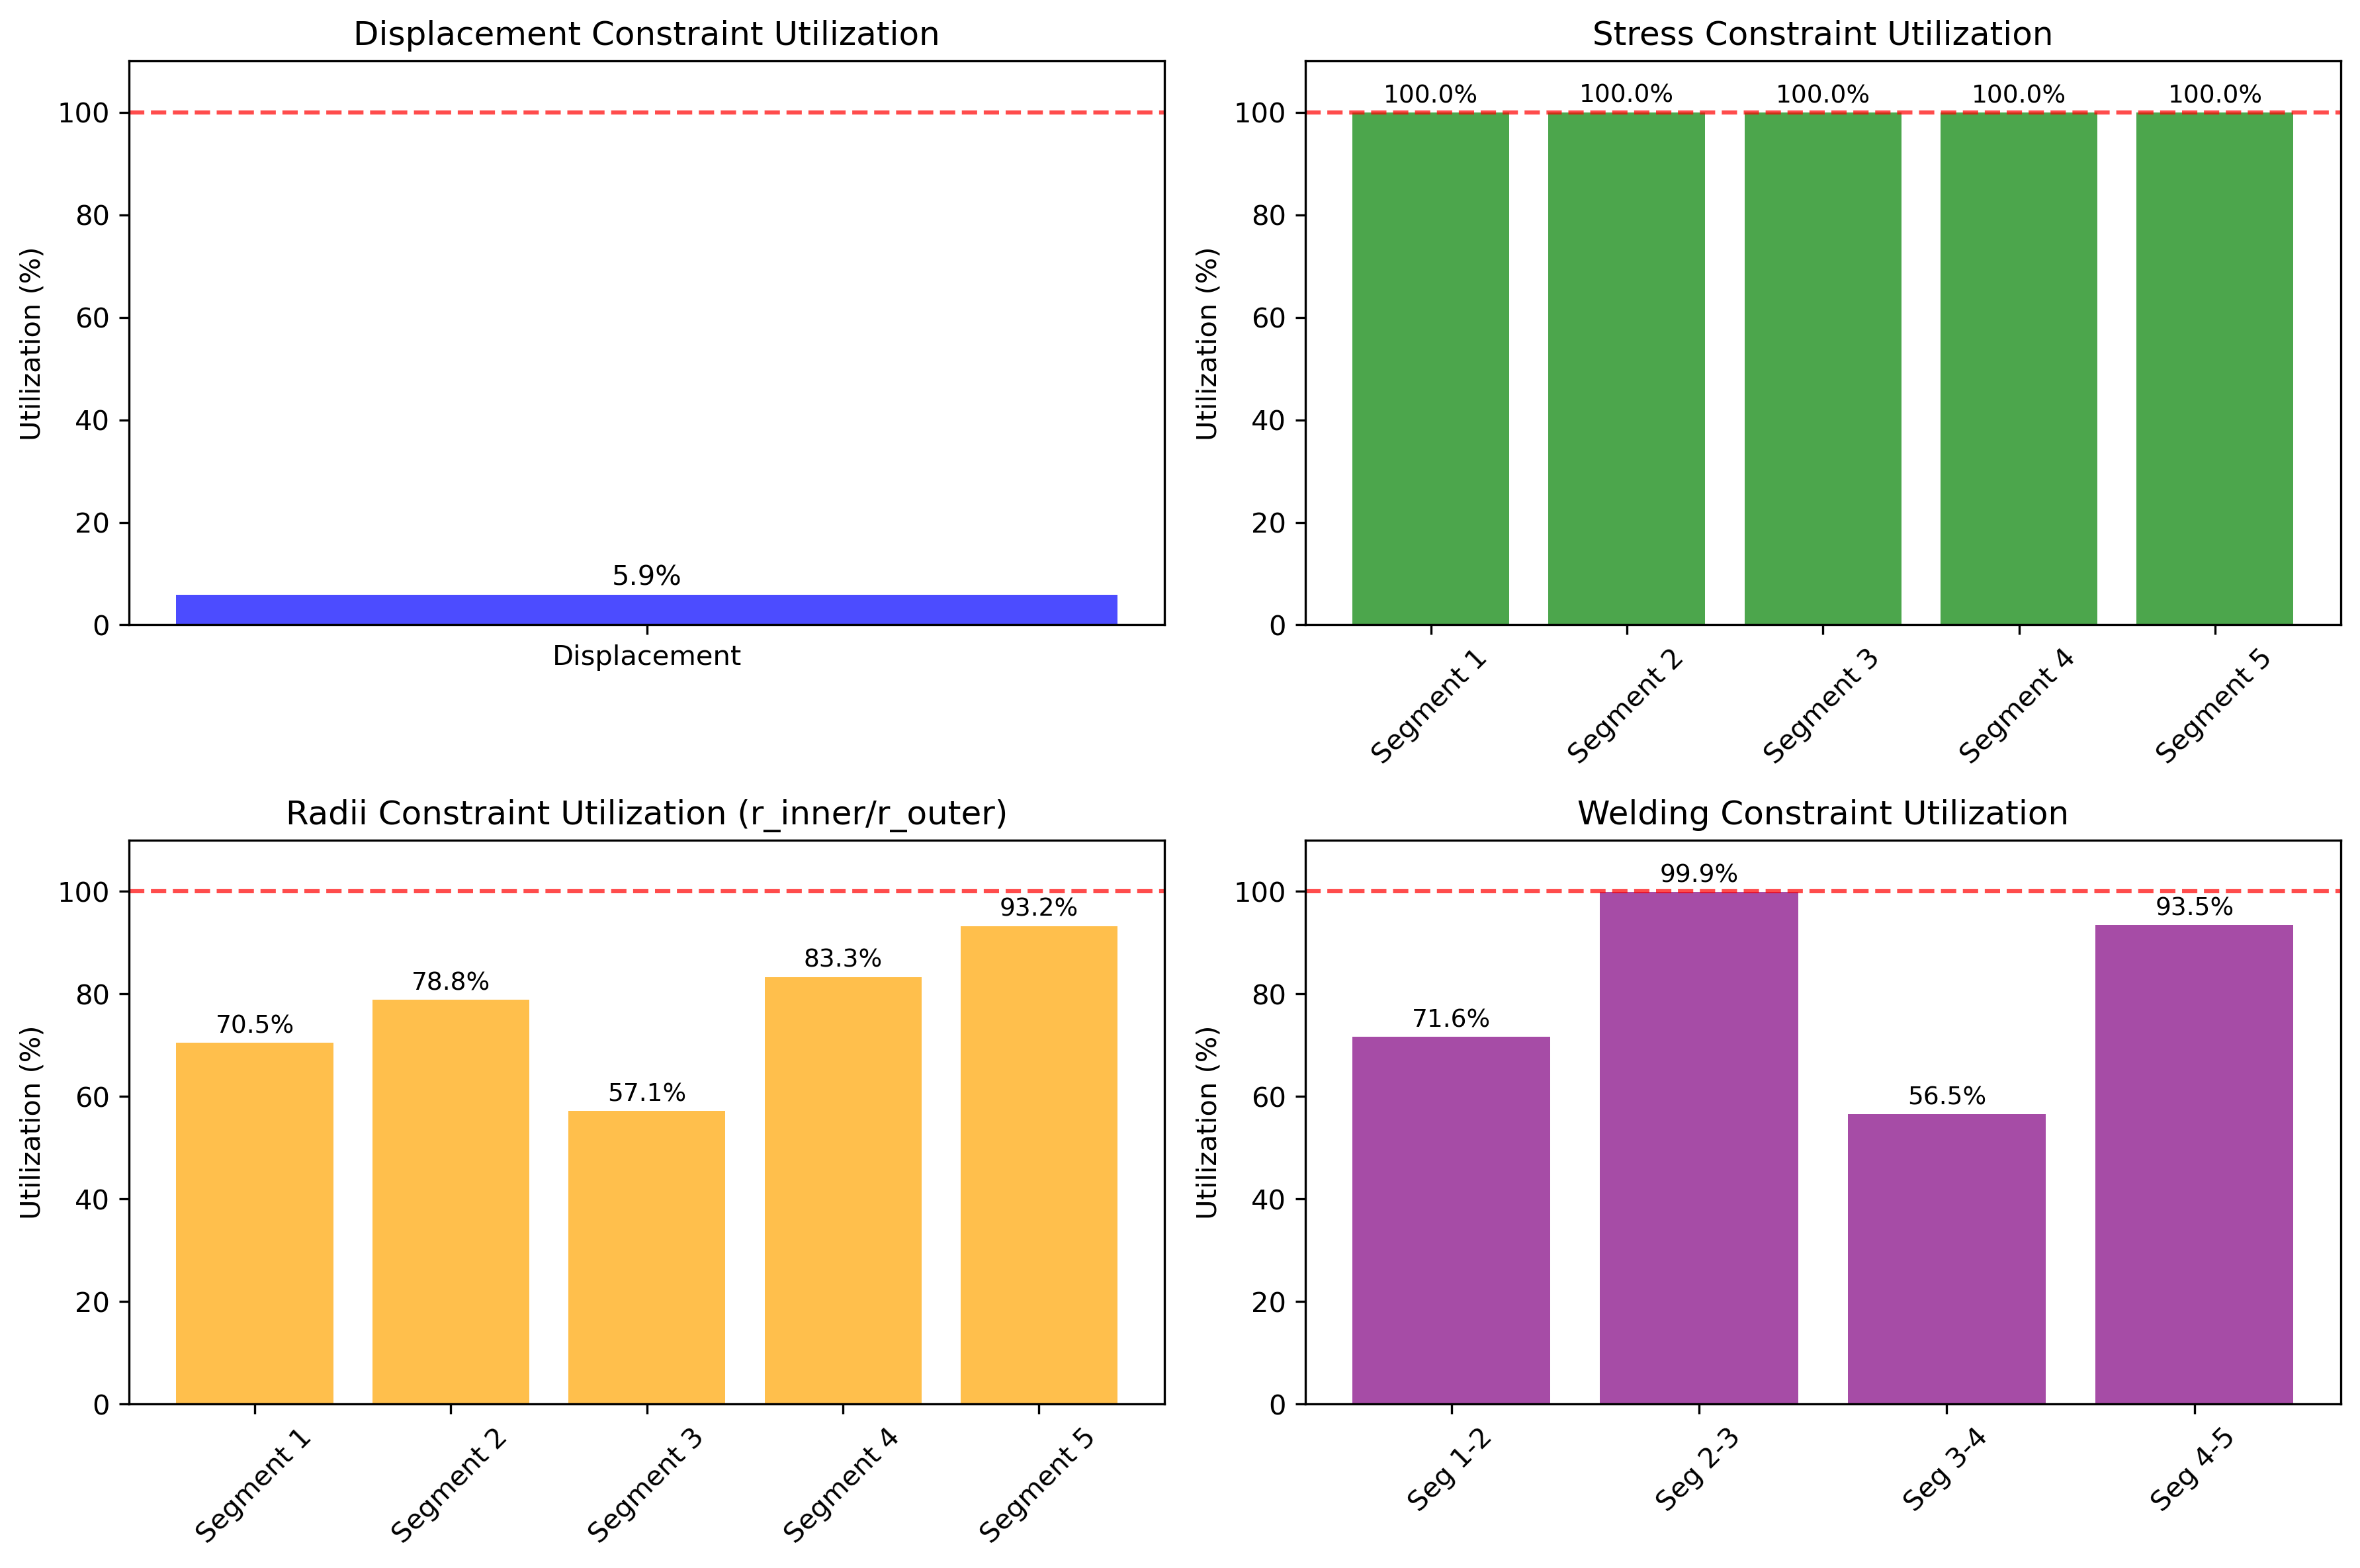
\includegraphics[width=1\textwidth]{weeks_new/imgs/constraint_utilization.png}
    \caption{Constraint Capacity Utilization Ratios}
    \label{fig:constraint_utilization}
\end{figure}

As can be seen from the graphs, the displacement constraint is active in the optimal design (fully utilized). This indicates that the optimized design has reached the limit in terms of weight minimization.

\subsection{Conclusion and Evaluation}
In this application, the optimal design of a cantilever beam for minimum weight under constraints has been obtained using the Simulated Annealing optimization algorithm. The results show that a structure 51\% lighter than the initial design has been achieved.

In the optimized design, it is observed that particularly the stress constraint is fully utilized (active). This is an expected theoretical result in weight minimization problems, as typically at least one constraint is expected to be active.

The gradual decrease in beam geometry from the support point towards the free end is also an expected structural result. Since the bending moment is maximum at the support point, larger cross-sections have formed in this region.   
\section{Uygulama II}
Bu bölümde SAP2000 OAPI kullanılarak 4 açıklıklı, 8 katlı basit bir çelik çerçevenin kesit optimizasyonu gerçekleştirilecektir. Optimizasyon işlemi için tavlama benzetimi algoritması kullanılacak ve LRFD yöntemine göre tasarım yapılacaktır.

\sidenote{
    
\qrcode[height=1in]{https://github.com/btayfur/structural-optimization/blob/main/Code/Examples/Exmp7/}}

\subsection{Çelik çerçeve modeli}
Model, 4 açıklıklı (5m açıklık mesafesi) ve 8 katlı (3m kat yüksekliği) bir çelik çerçeve yapıdan oluşmaktadır. Her katta açıklık üzerinde 40 kN/m düzgün yayılı yük bulunmaktadır. Tüm mesnetler ankastre olarak modellenmiştir. Yapıda Grade 36 çeliği kullanılmaktadır. Kirişlerin serbest burkulma boyu, kiriş uzunluğunun 1/5'i olarak kabul edilmiştir. SAP2000 Steel Design aracı kullanılarak tasarım ve optimizasyon işlemleri gerçekleştirilecektir.

\begin{figure}[H]
    \centering
    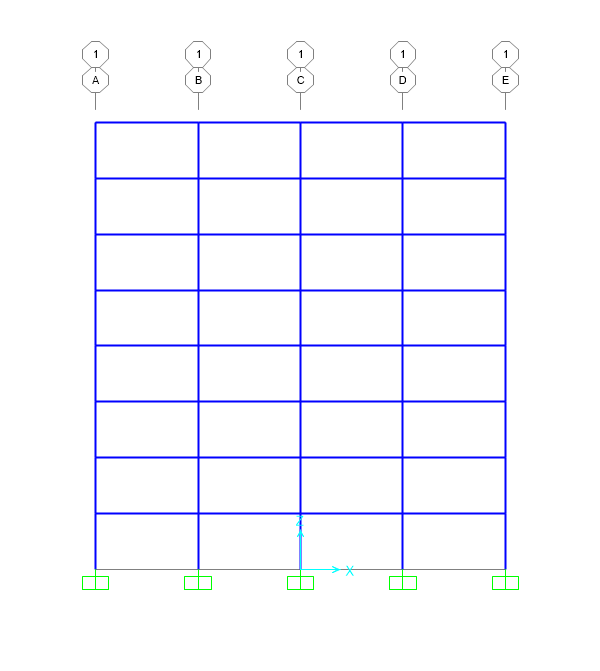
\includegraphics[width=0.8\textwidth]{weeks_new/imgs/exmp7_fig2.png}
    \caption{Çelik çerçeve modeli}
    \label{fig:model}
\end{figure}

\begin{figure}[H]
    \centering
    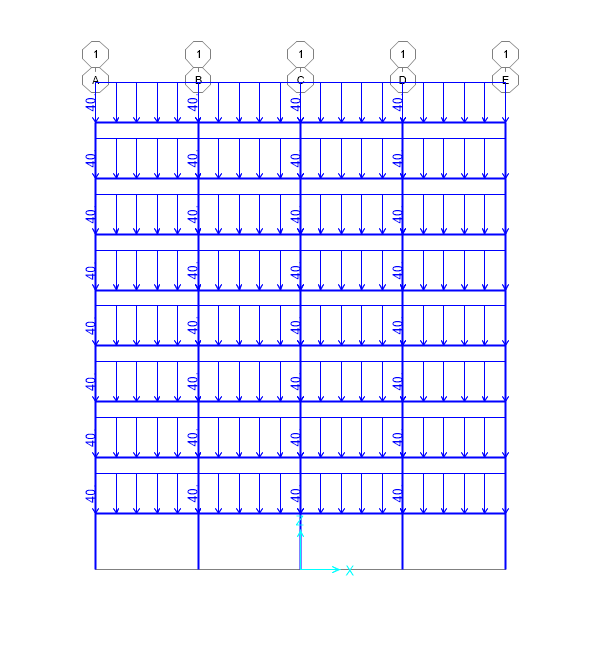
\includegraphics[width=0.8\textwidth]{weeks_new/imgs/exmp7_fig1.png}
    \caption{Yükleme Durumu}
    \label{fig:loading}
\end{figure}

\begin{figure}[H]
    \centering
    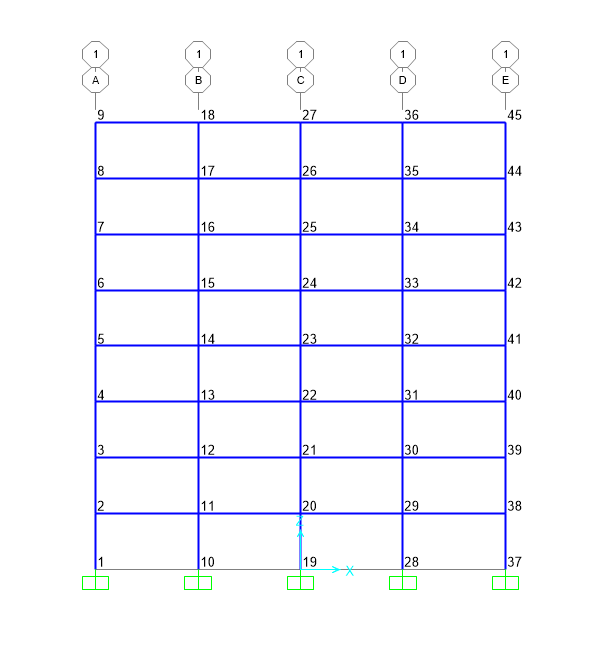
\includegraphics[width=0.8\textwidth]{weeks_new/imgs/exmp7_fig3.png}
    \caption{Düğüm noktalarının numaralandırılması}
    \label{fig:joints}
\end{figure}

\subsection{Kesit gruplandırması}
Yapıda kolon ve kirişler iki katta bir değişecek şekilde gruplandırılmıştır. Bu durumda toplam 4 kolon grubu ve 4 kiriş grubu bulunmaktadır. Her grup için farklı kesit seçimleri yapılacak ve optimizasyon sürecinde bu grupların kesitleri optimize edilecektir.

\subsubsection{Seçilebilir parametrelerin belirlenmesi}
Optimizasyon sürecinde kullanılacak kesit listesi, AISC kataloğundan seçilen W profillerinden oluşmaktadır. Kesit listesi W12'den W33'ye kadar farklı boyutlardaki profilleri içermektedir. Her grup için bu listeden uygun kesit seçimi yapılacak ve optimizasyon algoritması tarafından en uygun kesitler belirlenecektir.

\subsection{Optimizasyon}

\subsubsection{Amaç Fonksiyonu}
Optimizasyon sürecinde amaç fonksiyonu, yapının toplam ağırlığını minimize etmek olarak belirlenmiştir. Bu sayede hem ekonomik bir çözüm elde edilecek hem de yapının performansı optimize edilecektir.
Yapı ağırlığının hesaplamak için model içinde "weight" adlı bir "load case" oluşturulmuştur. Bu "load case" başka bir kuvvet barındırmadığından z eksenindeki mesnet reaksiyonları toplamı yapı ağırlığını verir. Bununla birlikte birçok yapısal optimizasyon probleminde olduğu gibi bu problemde de amaç fonksiyonu aşağıdaki gibi ifade edilebilir:

\begin{equation}
    f(x) = \sum_{i=1}^{n} \rho_i \cdot A_i \cdot L_i
\end{equation}
Burada $\rho_i$ kesit ağırlığını, $A_i$ kesit alanını ve $L_i$ kesit uzunluğunu ifade etmektedir. \sidenote{
    W kesitlerin kullanıldığı daha karmaşık problemlerde kesit isimlendirmesinden faydalanılabilir. Örneğin W12$\times$35 kesitinin $x35$ kısmı birim uzunluk başına ağırlığı ifade eder. Ancak bu değerlerin SI birimlerine çevrilmesi gerekmektedir.
}


\subsubsection{Sınırlayıcılar}
Optimizasyon sürecinde aşağıdaki sınırlayıcılar SAP2000 Çeelik Tasarım aracı kullanılarak gerçekleştirilir. VerifyPassed() metodu, yönetmelik şartlarını sağlamayan çerçeve elemanı sayısını döndürür. Arka planda ise burkulma boyundan genel bileşik denklemlere kadar tüm kontroller gerçekleştirilir. Ancak birçok optimizasyon çalışmasında -özellikle hız amacıyla OAPI ve benzeri araçların kullanılmadığı- aşağıdaki bileşik etki denklemleri kullanılarak kontroller sağlanır:
\begin{equation}
    \frac{P_u}{\phi_c P_n} \geq 0.2; \quad c_1=\frac{P_u}{\phi_c P_n} + \frac{8}{9} \left(\frac{M_{ux}}{\phi_b M_{nx}} + \frac{M_{uy}}{\phi_b M_{ny}}\right) 
\end{equation}
\begin{equation}
    \frac{P_u}{\phi_c P_n} < 0.2; \quad c_2=\frac{P_u}{\phi_c P_n} +  \left(\frac{M_{ux}}{\phi_b M_{nx}} + \frac{M_{uy}}{\phi_b M_{ny}}\right) 
\end{equation}
\begin{equation}
    \forall i: c_i \leq 1.0
\end{equation}

\subsection{Optimizasyon Sonuçları}
Tavlama benzetimi algoritması daha önce bahsedildiği gibi bir stokastik yöntemdir. Bu nedenle her çalıştırmada farklı sonuçların elde edilmesi doğaldır. Fakat araştırma amacıyla yapılan bir çalışmada algoritmanın tutarlığını sağlamak için genellikle çok sayıda çalıştırma yapılarak algoritmanın genel başarımı daha iyi anlaşılabilir. Bu örnekte yalnızca bir kez ve düşük sayılı iterasyon sınırı ile çalıştırma yapılacak ve sonuçları incelenecektir. Ancak yeterli analiz süresi tanındığında, örnek kapsamındaki kod da kolayca bu bağlamda değiştirilebilir.

\begin{figure}[H]
    \centering
    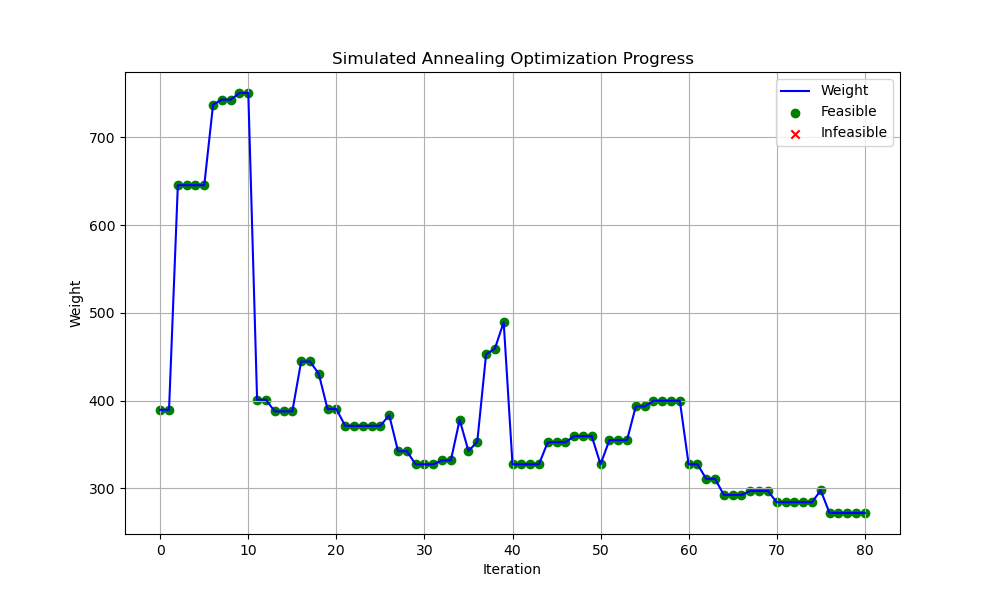
\includegraphics[width=0.8\textwidth]{weeks_new/imgs/exmp7_fig4.png}
    \caption{Yapı ağırlığının optimizasyon süresince değişimi}
    \label{fig:weight_change}
\end{figure}

\begin{table}
    \caption{Kiriş ve kolon kesitleri}
\end{table}

\begin{figure}[H]
    \centering
    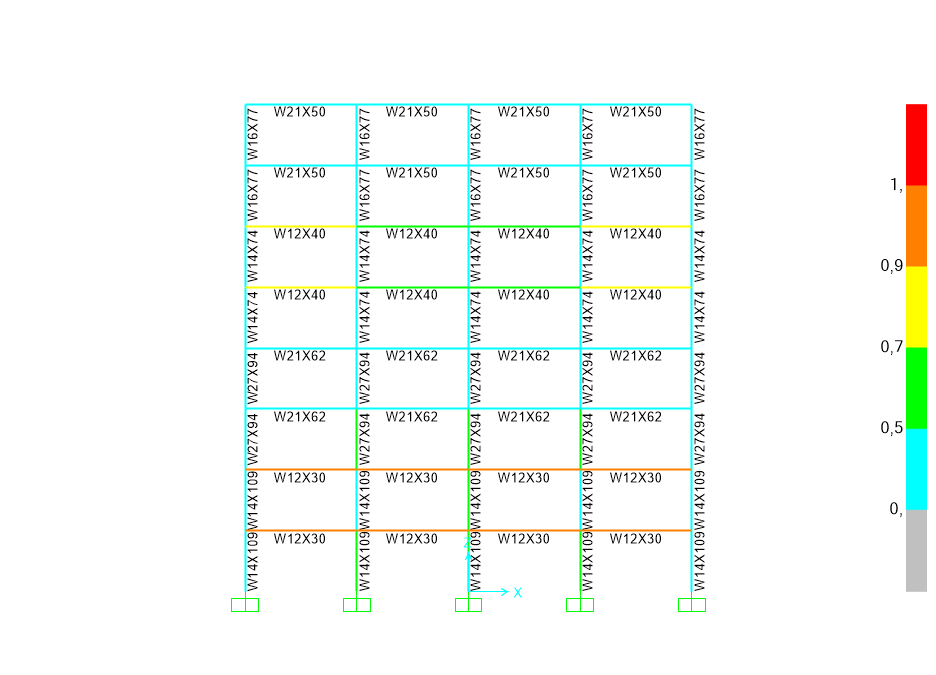
\includegraphics[width=0.8\textwidth]{weeks_new/imgs/exmp7_fig5.png}
    \caption{Optimum tasarımın Talep/Kapasite Oranı gösterimi}
    \label{fig:dcr_values}
\end{figure}





  

\end{document} 